\documentclass[conference]{IEEEtran}

% =========================================================
% PARÁMETROS CONFIGURABLES POR SEMANA
% =========================================================
\newcommand{\NumeroSemana}{05}
\newcommand{\TemaSemana}{Integración de algunas funciones irracional}

% --- PAQUETES BÁSICOS Y MATEMÁTICOS ---
\usepackage[utf8]{inputenc}
\usepackage[T1]{fontenc}
\usepackage{amsmath,amssymb,amsfonts}
\usepackage{mathtools}
\usepackage{graphicx}
\usepackage{hyperref}
\usepackage{float}
\usepackage{array}

% --- RUTA BÁSICA DE IMÁGENES ---
\graphicspath{{semana_05/graficas/}}

\begin{document}
	
	% =========================================================
	% PORTADA OFICIAL FORMATO IEEE - FIEE UNMSM
	% =========================================================
	\title{UNIVERSIDAD NACIONAL MAYOR DE SAN MARCOS\\
		\Large FACULTAD DE INGENIERÍA ELECTRÓNICA Y ELÉCTRICA (FIEE)\\
		\vspace{0.3cm}
		\large \textbf{Curso:} Cálculo II (Cálculo Integral) \quad|\quad \textbf{Docente:} Dr. Raúl Castro Vidal\\
		\vspace{0.4cm}
		\huge SOLUCIÓN DE EJERCICIOS PROPUESTOS --- SEMANA \NumeroSemana\\
		\LARGE INFORME TÉCNICO GRUPAL: \TemaSemana}
	
	% --- BLOQUE DE AUTORES ---
	\author{
		\IEEEauthorblockN{Coordinador: Adrián Córdova Suazo}
		\IEEEauthorblockA{\textit{Código: 26190164} \\
			\textit{Ing. Electrónica}}
		\and
		\IEEEauthorblockN{Integrante 2: Diego Checcori Cuya}
		\IEEEauthorblockA{\textit{Código: 26190008} \\
			\textit{Ing. Electrónica}}
		\and
		\IEEEauthorblockN{Integrante 3: Diego Anamaria Choque}
		\IEEEauthorblockA{\textit{Código: 26190001} \\
			\textit{Ing. Electrónica}}
		\vspace{0.4cm}
		\and
		\IEEEauthorblockN{Integrante 4: Deyvis Tenorio Yucra}
		\IEEEauthorblockA{\textit{Código: 26190199} \\
			\textit{Ing. Electrónica}}
		\and
		\IEEEauthorblockN{Integrante 5: Felix Chocce Oseda}
		\IEEEauthorblockA{\textit{Código: 23190231} \\
			\textit{Ing. Eléctrica}}
		\and
		\IEEEauthorblockN{Integrante 6: Isaac Guadalupe Baños}
		\IEEEauthorblockA{\textit{Código: 26190169} \\
			\textit{Ing. Electrónica}}
	}
	
	\maketitle
	
	\begin{abstract}
		En el presente informe técnico correspondiente a la asignatura de Cálculo II, a cargo del Dr. Raúl Castro Vidal, se presenta la solución analítica paso a paso de los ejercicios propuestos para la Semana \NumeroSemana. Cada problema incluye su representación y análisis gráfico desarrollado en Matplotlib evaluado en la constante de integración $C=0$, estructurado formalmente bajo los estándares IEEE a dos columnas.
	\end{abstract}
	
	\begin{IEEEkeywords}
		Cálculo II, \TemaSemana, Matplotlib, Formato IEEE, FIEE-UNMSM.
	\end{IEEEkeywords}
	
	\section{Desarrollo de los Ejercicios}
	
	% --- LISTA DIRECTA CON RUTAS EXPLÍCITAS ---
	\subsection*{Problema 01}

\noindent\textbf{Enunciado:} Calcular la integral:
\begin{align*}
\int -\dfrac{\sqrt[4]{x}}{\sqrt{x}(1 + \sqrt[4]{x})} \, dx
\end{align*}

\noindent\textbf{Solución:} Para resolver esta integral, aplicamos la sustitución sugerida. Sea $u = \sqrt[4]{x}$, de donde se deduce que $x = u^4$ y el diferencial es $dx = 4u^3 \, du$. Además, notamos que $\sqrt{x} = (u^4)^{1/2} = u^2$.

Sustituyendo estas expresiones en la integral original, obtenemos:
\begin{align*}
I &= \int -\dfrac{u}{u^2(1 + u)} (4u^3 \, du)
\end{align*}

Simplificamos la expresión algebraica dentro del integrando dividiendo $u^3$ entre $u^2$:
\begin{align*}
I &= -4 \int \dfrac{u^4}{u^2(1 + u)} \, du \\
I &= -4 \int \dfrac{u^2}{1 + u} \, du
\end{align*}

Como el grado del numerador es mayor que el del denominador, realizamos la división polinómica o un ajuste algebraico sumando y restando $1$ en el numerador:
\begin{align*}
\dfrac{u^2}{1 + u} &= \dfrac{u^2 - 1 + 1}{1 + u} \\
&= \dfrac{(u - 1)(u + 1)}{1 + u} + \dfrac{1}{1 + u} \\
&= u - 1 + \dfrac{1}{1 + u}
\end{align*}

Reemplazamos esto en nuestra integral:
\begin{align*}
I &= -4 \int \left( u - 1 + \dfrac{1}{1 + u} \right) du
\end{align*}

Integramos término a término:
\begin{align*}
I &= -4 \left( \dfrac{u^2}{2} - u + \ln|1 + u| \right) + C \\
I &= -2u^2 + 4u - 4\ln|1 + u| + C
\end{align*}

Finalmente, regresamos a la variable original $x$ sustituyendo $u = \sqrt[4]{x}$:
\begin{align*}
I &= -2(\sqrt[4]{x})^2 + 4\sqrt[4]{x} \\
&\quad - 4\ln|1 + \sqrt[4]{x}| + C \\
I &= -2\sqrt{x} + 4\sqrt[4]{x} \\
&\quad - 4\ln|1 + \sqrt[4]{x}| + C
\end{align*}

\begin{figure}[H]
	\centering
	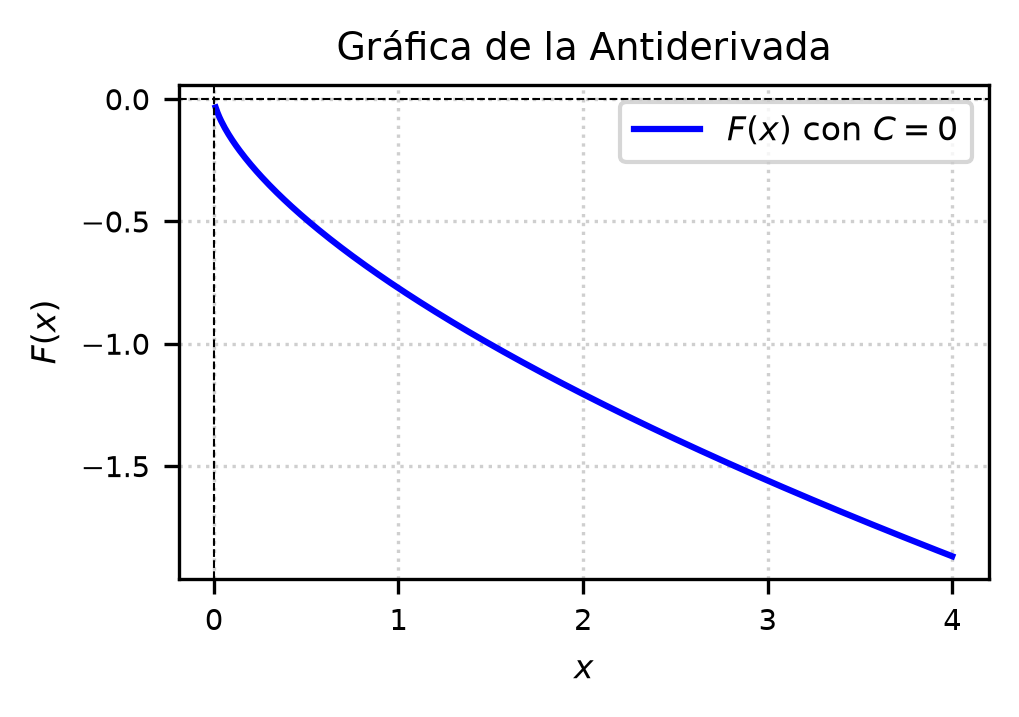
\includegraphics[width=\columnwidth]{semana_05/graficas/SEM05_P01_grafica.png}
	\caption{Representación gráfica de $f(x)$ y su antiderivada $F(x)$ evaluada para la constante de integración $C = 0$ (Problema 01).}
	\label{fig:problema01}
\end{figure}

	\subsection*{Problema 02}

\textbf{Enunciado:} Calcular la integral:
\begin{align*}
\int \sqrt[3]{x^2} \left(-1 + 2\sqrt[3]{x}\right)^3 \, dx
\end{align*}

\textbf{Solución:} 
Primero, reescribimos las raíces utilizando exponentes fraccionarios. Sabemos que $\sqrt[3]{x^2} = x^{2/3}$ y $\sqrt[3]{x} = x^{1/3}$. La integral se expresa como:
\begin{align*}
I = \int x^{2/3} \left(-1 + 2x^{1/3}\right)^3 \, dx
\end{align*}

A continuación, desarrollamos el binomio al cubo utilizando la fórmula $(a + b)^3 = a^3 + 3a^2b + 3ab^2 + b^3$, donde $a = -1$ y $b = 2x^{1/3}$:
\begin{align*}
\left(-1 + 2x^{1/3}\right)^3 &= (-1)^3 + 3(-1)^2(2x^{1/3}) \\
&\quad + 3(-1)(2x^{1/3})^2 + (2x^{1/3})^3
\end{align*}

Simplificando cada uno de los términos del desarrollo anterior:
\begin{align*}
\left(-1 + 2x^{1/3}\right)^3 &= -1 + 6x^{1/3} \\
&\quad - 12x^{2/3} + 8x
\end{align*}

Sustituimos este resultado en la integral original y multiplicamos por el término $x^{2/3}$ que se encuentra afuera:
\begin{align*}
I &= \int x^{2/3} \Big(-1 + 6x^{1/3} \\
&\quad - 12x^{2/3} + 8x \Big) \, dx
\end{align*}

Distribuimos $x^{2/3}$ en cada término y sumamos los exponentes correspondientes:
\begin{align*}
I &= \int \left( -x^{2/3} + 6x^{3/3} - 12x^{4/3} + 8x^{5/3} \right) \, dx \\
I &= \int \left( -x^{2/3} + 6x - 12x^{4/3} + 8x^{5/3} \right) \, dx
\end{align*}

Ahora, integramos cada término aplicando la regla de las potencias $\int x^n \, dx = \dfrac{x^{n+1}}{n+1}$:
\begin{align*}
\int -x^{2/3} \, dx &= -\dfrac{x^{5/3}}{\frac{5}{3}} = -\dfrac{3}{5}x^{5/3}
\end{align*}
\begin{align*}
\int 6x \, dx &= 6\dfrac{x^2}{2} = 3x^2
\end{align*}
\begin{align*}
\int -12x^{4/3} \, dx &= -12\dfrac{x^{7/3}}{\frac{7}{3}} = -\dfrac{36}{7}x^{7/3}
\end{align*}
\begin{align*}
\int 8x^{5/3} \, dx &= 8\dfrac{x^{8/3}}{\frac{8}{3}} = 3x^{8/3}
\end{align*}

Juntando todos los resultados y agregando la constante de integración $C$, obtenemos la solución general:
\begin{align*}
I &= -\dfrac{3}{5}x^{5/3} + 3x^2 \\
&\quad -\dfrac{36}{7}x^{7/3} + 3x^{8/3} + C
\end{align*}

\begin{figure}[H]
	\centering
	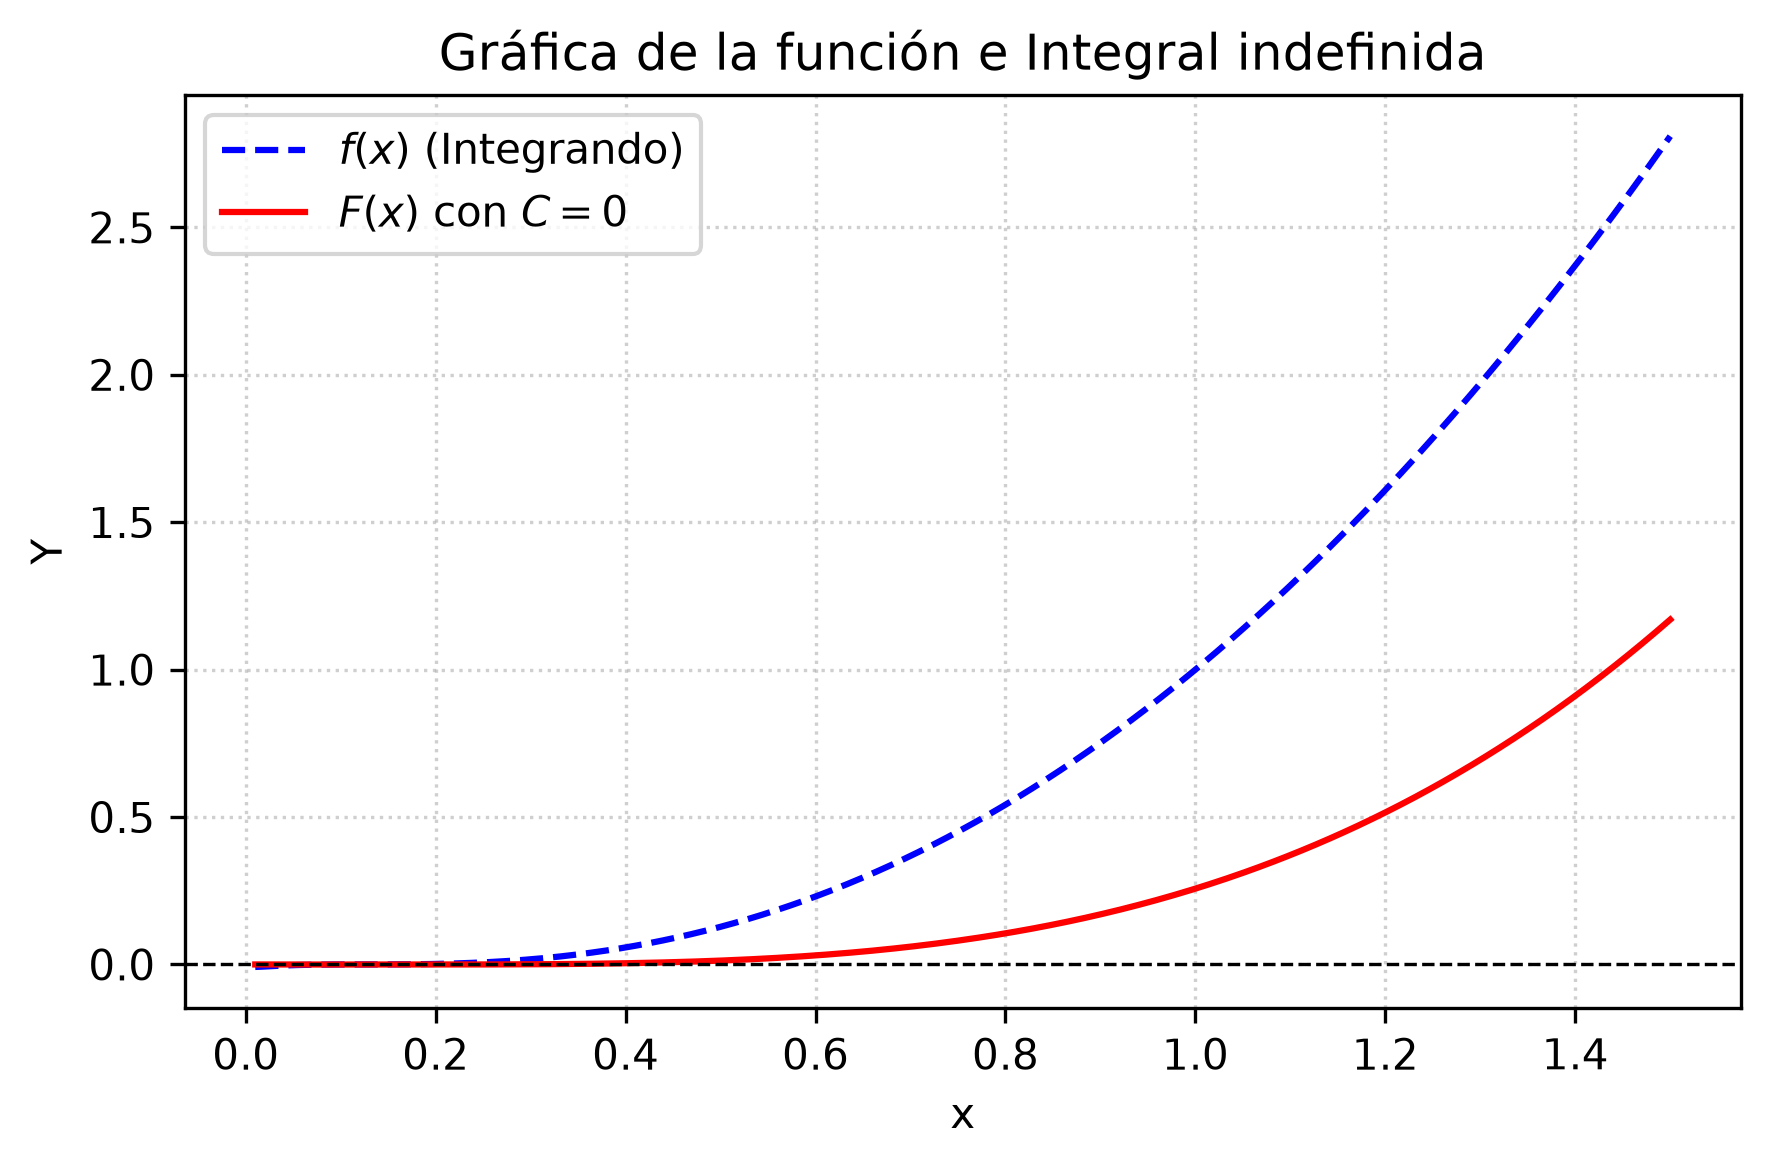
\includegraphics[width=\columnwidth]{semana_05/graficas/SEM05_P02_grafica.png}
	\caption{Representación gráfica de $f(x)$ y su antiderivada $F(x)$ evaluada para la constante de integración $C = 0$ (Problema 02).}
	\label{fig:problema02}
\end{figure}

	\subsection*{Problema 03}

\textbf{Enunciado:} \\
Calcular la integral indefinida:
\begin{align*}
\int x^3 (1 - x^2)^{-\frac{3}{2}} \, dx
\end{align*}

\textbf{Solución:} \\
Para resolver esta integral, utilizaremos el método de sustitución algebraica. 
Definimos el cambio de variable:
\begin{align*}
u &= 1 - x^2 \\
du &= -2x \, dx
\end{align*}

De la definición de $u$, podemos expresar $x^2$ en términos de $u$:
\begin{align*}
x^2 = 1 - u
\end{align*}

Además, despejamos el producto $x \, dx$ para adaptarlo al integrando:
\begin{align*}
x \, dx = -\frac{1}{2} \, du
\end{align*}

Reescribimos la integral original separando un factor $x$:
\begin{align*}
\int x^3 (1 - x^2)^{-\frac{3}{2}} \, dx &= \int (x^2) (1 - x^2)^{-\frac{3}{2}} (x \, dx)
\end{align*}

Sustituimos las expresiones en términos de $u$:
\begin{align*}
&= \int (1 - u) (u)^{-\frac{3}{2}} \left(-\frac{1}{2} \, du\right) \\
&= -\frac{1}{2} \int (1 - u) u^{-\frac{3}{2}} \, du
\end{align*}

Multiplicamos el término $u^{-\frac{3}{2}}$ dentro del paréntesis:
\begin{align*}
&= -\frac{1}{2} \int \left( u^{-\frac{3}{2}} - u^{-\frac{1}{2}} \right) du
\end{align*}

Integramos cada término aplicando la regla de la potencia:
\begin{align*}
&= -\frac{1}{2} \left( \frac{u^{-\frac{1}{2}}}{-\frac{1}{2}} - \frac{u^{\frac{1}{2}}}{\frac{1}{2}} \right) + C \\
&= -\frac{1}{2} \left( -2u^{-\frac{1}{2}} - 2u^{\frac{1}{2}} \right) + C
\end{align*}

Simplificamos los coeficientes:
\begin{align*}
&= u^{-\frac{1}{2}} + u^{\frac{1}{2}} + C
\end{align*}

Regresamos a la variable original $x$ sustituyendo $u = 1 - x^2$:
\begin{align*}
&= (1 - x^2)^{-\frac{1}{2}} + (1 - x^2)^{\frac{1}{2}} + C
\end{align*}

Expresando el resultado en forma de radicales, obtenemos la solución final:
\begin{align*}
&= \dfrac{1}{\sqrt{1 - x^2}} + \sqrt{1 - x^2} + C
\end{align*}

\begin{figure}[H]
	\centering
	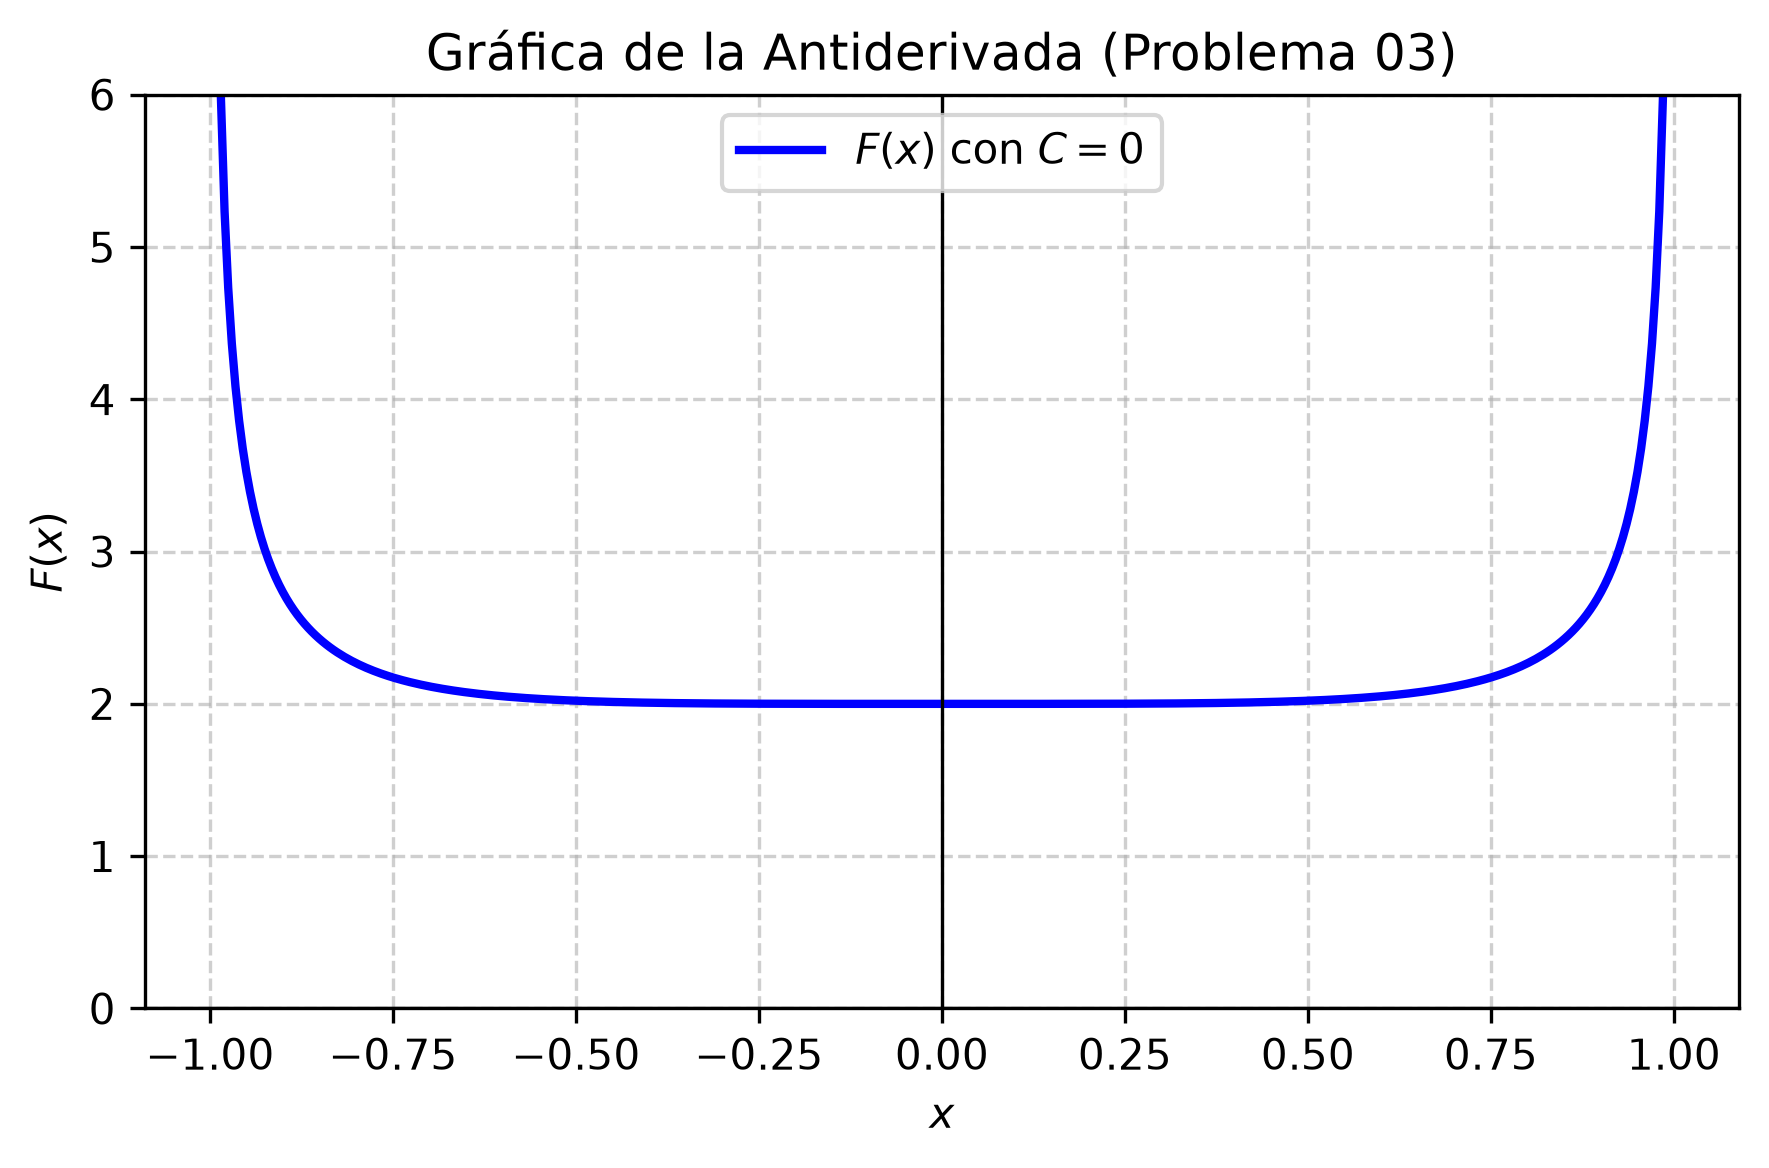
\includegraphics[width=\columnwidth]{semana_05/graficas/SEM05_P03_grafica.png}
	\caption{Representación gráfica de $f(x)$ y su antiderivada $F(x)$ evaluada para la constante de integración $C = 0$ (Problema 03).}
	\label{fig:problema03}
\end{figure}

	\subsection*{Problema 04}

\textbf{Enunciado:} \\
Calcular la integral indefinida:
\begin{align*}
\int x^3 (1 + x^2)^{-\frac{1}{2}} \, dx
\end{align*}

\textbf{Solución:} \\
Siguiendo las indicaciones, realizamos
la sustitución sugerida. Definimos:
\begin{align*}
u = \sqrt{1 + x^2}
\end{align*}

Elevando al cuadrado ambos lados y
despejando $x^2$, obtenemos:
\begin{align*}
u^2 = 1 + x^2 \implies x^2 = u^2 - 1
\end{align*}

Ahora, diferenciamos ambos lados de la
expresión para encontrar $dx$:
\begin{align*}
2u \, du = 2x \, dx \implies x \, dx = u \, du
\end{align*}

Reescribimos la integral original
separando un factor $x$ para usar $dx$:
\begin{align*}
I &= \int x^2 (1 + x^2)^{-\frac{1}{2}} (x \, dx)
\end{align*}

Sustituimos $x^2 = u^2 - 1$,
$1 + x^2 = u^2$ y $x \, dx = u \, du$:
\begin{align*}
I &= \int (u^2 - 1) (u^2)^{-\frac{1}{2}} (u \, du)
\end{align*}

Simplificamos el término algebraico:
\begin{align*}
(u^2)^{-\frac{1}{2}} = \dfrac{1}{\sqrt{u^2}} = \dfrac{1}{u}
\end{align*}

Sustituimos esto en la integral:
\begin{align*}
I &= \int (u^2 - 1) \left(\dfrac{1}{u}\right) u \, du \\
I &= \int (u^2 - 1) \, du
\end{align*}

Integramos término a término respecto a $u$:
\begin{align*}
I &= \int u^2 \, du - \int 1 \, du \\
I &= \dfrac{u^3}{3} - u + C
\end{align*}

Finalmente, regresamos a la variable
original $x$ sustituyendo $u = \sqrt{1 + x^2}$:
\begin{align*}
I &= \dfrac{(\sqrt{1 + x^2})^3}{3} \\
  &\quad - \sqrt{1 + x^2} + C
\end{align*}

Expresando el resultado final de
forma compacta:
\begin{align*}
I &= \dfrac{(1 + x^2)^{\frac{3}{2}}}{3} \\
  &\quad - (1 + x^2)^{\frac{1}{2}} + C
\end{align*}

\begin{figure}[H]
	\centering
	
\includegraphics[width=\columnwidth]{semana_05/graficas/SEM05_P04_grafica.png}
	\caption{Representación gráfica de $f(x)$ y su antiderivada $F(x)$ evaluada para la constante de integración $C = 0$ (Problema 04).}
	\label{fig:problema04}
\end{figure}

	\subsection*{Problema 05}

\textbf{Enunciado:} Calcular la integral indefinida
\begin{align*}
\int \dfrac{x}{\sqrt{x} - 1} \, dx
\end{align*}

\textbf{Solución:} Siguiendo las indicaciones, aplicamos la sustitución $u = \sqrt{x}$. 
De aquí obtenemos que $x = u^2$ y el diferencial es:
\begin{align*}
dx = 2u \, du
\end{align*}

Sustituimos estas expresiones en la integral original:
\begin{align*}
I &= \int \dfrac{u^2}{u - 1} (2u \, du) \\
I &= 2 \int \dfrac{u^3}{u - 1} \, du
\end{align*}

El integrando es un cociente de polinomios donde el grado del numerador es mayor que el del denominador. Realizamos la división algebraica de $u^3$ entre $u - 1$. 

Dividiendo $u^3$ por $u - 1$:
\begin{align*}
\dfrac{u^3}{u - 1} = u^2 + u + 1 + \dfrac{1}{u - 1}
\end{align*}

Sustituimos este resultado en nuestra integral:
\begin{align*}
I &= 2 \int \left( u^2 + u + 1 + \dfrac{1}{u - 1} \right) du
\end{align*}

integramos término a término:
\begin{align*}
I &= 2 \left( \dfrac{u^3}{3} + \dfrac{u^2}{2} + u + \ln|u - 1| \right) + C
\end{align*}

Multiplicamos por el factor $2$:
\begin{align*}
I &= \dfrac{2}{3}u^3 + u^2 + 2u \\
&\quad + 2\ln|u - 1| + C
\end{align*}

Finalmente, regresamos a la variable original sustituyendo $u = \sqrt{x}$:
\begin{align*}
I &= \dfrac{2}{3}(\sqrt{x})^3 + (\sqrt{x})^2 \\
&\quad + 2\sqrt{x} + 2\ln|\sqrt{x} - 1| + C
\end{align*}

Simplificando los exponentes, el resultado final de la integral es:
\begin{align*}
\int \dfrac{x}{\sqrt{x} - 1} \, dx &= \dfrac{2}{3}x^{3/2} + x + 2\sqrt{x} \\
&\quad + 2\ln|\sqrt{x} - 1| + C
\end{align*}

\begin{figure}[H]
	\centering
	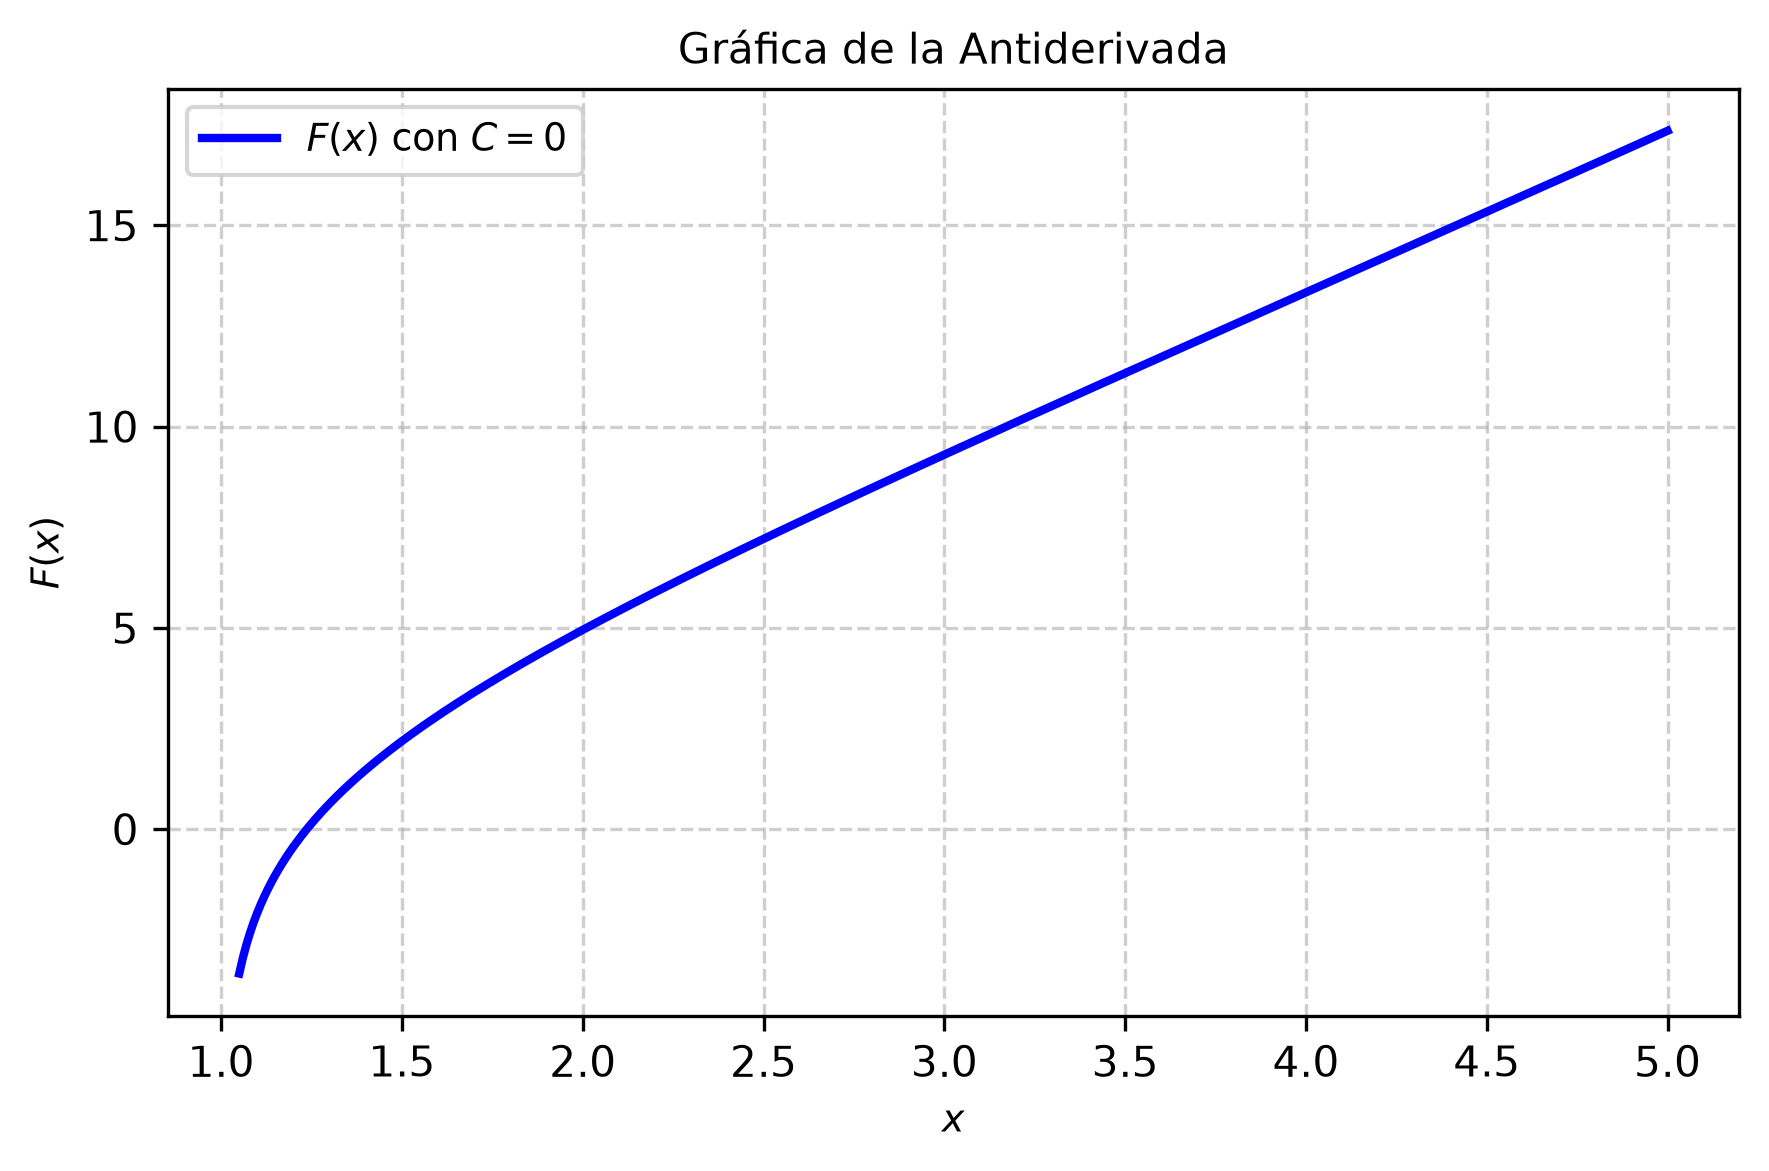
\includegraphics[width=\columnwidth]{semana_05/graficas/SEM05_P05_grafica.png}
	\caption{Representación gráfica de $f(x)$ y su antiderivada $F(x)$ evaluada para la constante de integración $C = 0$ (Problema 05).}
	\label{fig:problema05}
\end{figure}

	\subsection*{Problema 06}

\textbf{Enunciado:} Calcular la integral:
\begin{align*}
\int \dfrac{\sqrt{x}}{x - 1} \, dx
\end{align*}

\textbf{Solución:} Siguiendo la indicación, 
realizamos el cambio de variable:
\begin{align*}
u &= \sqrt{x}, \quad x = u^2 \\
dx &= 2u \, du
\end{align*}

Sustituyendo en la integral original, 
obtenemos:
\begin{align*}
\int \dfrac{\sqrt{x}}{x - 1} \, dx &= \int \dfrac{u}{u^2 - 1} (2u \, du) \\
&= \int \dfrac{2u^2}{u^2 - 1} \, du
\end{align*}

Dado que el grado del numerador es igual 
al del denominador, dividimos la fracción 
algebraica o reescribimos el integrando:
\begin{align*}
\dfrac{2u^2}{u^2 - 1} &= \dfrac{2u^2 - 2 + 2}{u^2 - 1} \\
&= 2 + \dfrac{2}{u^2 - 1}
\end{align*}

Expandimos el término restante usando 
fracciones parciales:
\begin{align*}
\dfrac{2}{(u-1)(u+1)} &= \dfrac{A}{u-1} + \dfrac{B}{u+1}
\end{align*}

Resolviendo para los coeficientes, 
encontramos que $A = 1$ y $B = -1$. 
Entonces, la integral se descompone en:
\begin{align*}
\int \left( 2 + \dfrac{1}{u-1} - \dfrac{1}{u+1} \right) du
\end{align*}

Integramos término a término:
\begin{align*}
&= 2u + \ln|u-1| - \ln|u+1| + C \\
&= 2u + \ln\left|\dfrac{u-1}{u+1}\right| + C
\end{align*}

Finalmente, regresamos a la variable 
original $x$ sustituyendo $u = \sqrt{x}$:
\begin{align*}
= 2\sqrt{x} + \ln\left|\dfrac{\sqrt{x}-1}{\sqrt{x}+1}\right| + C
\end{align*}

\begin{figure}[H]
	\centering
	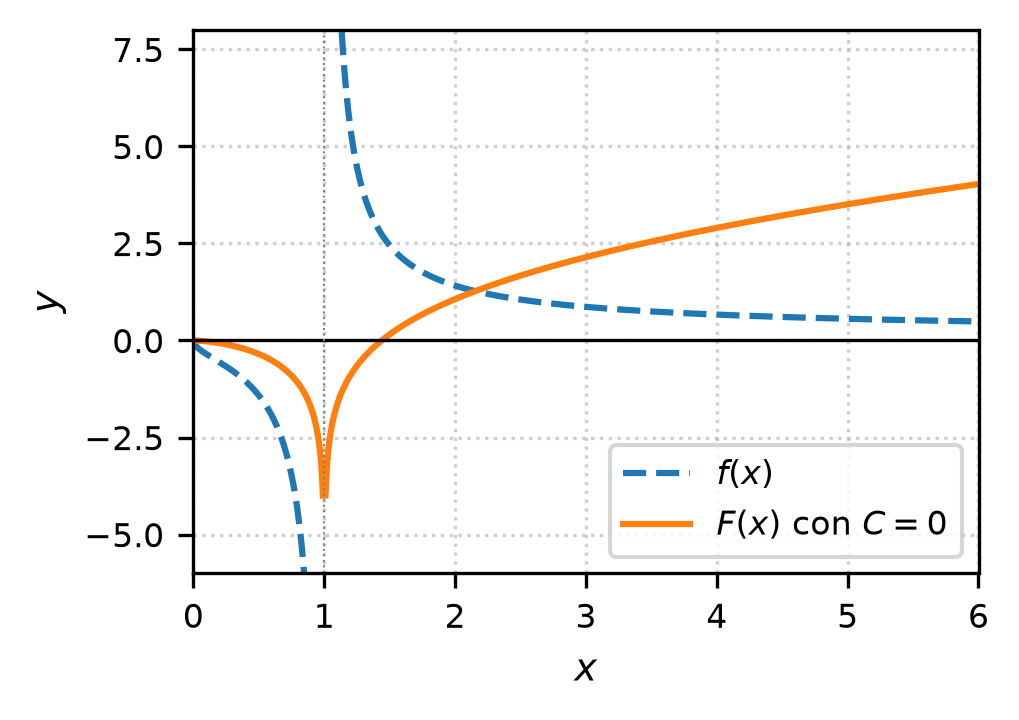
\includegraphics[width=\columnwidth]{semana_05/graficas/SEM05_P06_grafica.png}
	\caption{Representación gráfica de $f(x)$ y su antiderivada $F(x)$ evaluada para la constante de integración $C = 0$ (Problema 06).}
	\label{fig:problema06}
\end{figure}

	\subsection*{Problema 07}

\textbf{Enunciado:} Calcular la integral:
\begin{equation*}
  \int \frac{dx}{\sqrt{4x^2 + 4x - 3}}
\end{equation*}

\textbf{Solución:} 

Comenzamos completando el cuadrado 
dentro de la expresión radical del 
denominador. Tomamos la expresión 
cuadrática:
\begin{align*}
  4x^2 + 4x - 3 &= 4(x^2 + x) - 3 \\
  &= 4\left(x^2 + x + \frac{1}{4} - \frac{1}{4}\right) - 3 \\
  &= 4\left(x + \frac{1}{2}\right)^2 - 1 - 3 \\
  &= 4\left(x + \frac{1}{2}\right)^2 - 4
\end{align*}

También podemos escribirlo como:
\begin{equation*}
  4x^2 + 4x - 3 = (2x + 1)^2 - 4
\end{equation*}

Sustituyendo esto en la integral 
original, obtenemos:
\begin{align*}
  I &= \int \frac{dx}{\sqrt{(2x + 1)^2 - 4}}
\end{align*}

Utilizamos la sustitución 
trigonométrica secante. 
Hacemos el cambio de variable:
\begin{equation*}
  2x + 1 = 2\sec\theta
\end{equation*}

Derivando ambos lados para 
encontrar el diferencial $dx$:
\begin{align*}
  2\,dx &= 2\sec\theta\tan\theta\,d\theta \\
  dx &= \sec\theta\tan\theta\,d\theta
\end{align*}

Sustituimos $2x + 1$ y $dx$ 
en la integral:
\begin{align*}
  I &= \int \frac{\sec\theta\tan\theta\,d\theta}{\sqrt{(2\sec\theta)^2 - 4}} \\
  &= \int \frac{\sec\theta\tan\theta\,d\theta}{\sqrt{4(\sec^2\theta - 1)}}
\end{align*}

Empleamos la identidad trigonométrica 
fundamental $\sec^2\theta - 1 = \tan^2\theta$:
\begin{align*}
  I &= \int \frac{\sec\theta\tan\theta\,d\theta}{\sqrt{4\tan^2\theta}} \\
  &= \int \frac{\sec\theta\tan\theta\,d\theta}{2\tan\theta} \\
  &= \frac{1}{2}\int \sec\theta\,d\theta
\end{align*}

La integral de la secante es un 
resultado estándar conocido:
\begin{equation*}
  I = \frac{1}{2}\ln\left|\sec\theta + \tan\theta\right| + C
\end{equation*}

A partir de la sustitución original 
$2x + 1 = 2\sec\theta$, despejamos 
la secante:
\begin{equation*}
  \sec\theta = \frac{2x + 1}{2}
\end{equation*}

Para encontrar $\tan\theta$, 
utilizamos la identidad 
$\tan\theta = \sqrt{\sec^2\theta - 1}$:
\begin{align*}
  \tan\theta &= \sqrt{\left(\frac{2x + 1}{2}\right)^2 - 1} \\
  &= \sqrt{\frac{4x^2 + 4x + 1 - 4}{4}} \\
  &= \frac{\sqrt{4x^2 + 4x - 3}}{2}
\end{align*}

Sustituimos las expresiones 
de $\sec\theta$ y $\tan\theta$ 
en términos de $x$:
\begin{align*}
  I &= \frac{1}{2}\ln\left|
  \frac{2x + 1}{2} + \frac{\sqrt{4x^2 + 4x - 3}}{2}
  \right| + C
\end{align*}

Aplicando propiedades de los 
logaritmos para simplificar 
la constante del denominador:
\begin{align*}
  I &= \frac{1}{2}\ln\left|
  2x + 1 + \sqrt{4x^2 + 4x - 3}
  \right| \\
  &\quad - \frac{1}{2}\ln(2) + C
\end{align*}

Agrupando la constante $-\frac{1}{2}\ln(2)$ 
con la constante de integración $C$, 
obtenemos la solución general final:
\begin{align*}
  I &= \frac{1}{2}\ln\left|
  2x + 1 + \sqrt{4x^2 + 4x - 3}
  \right| + C
\end{align*}

\begin{figure}[H]
	\centering
	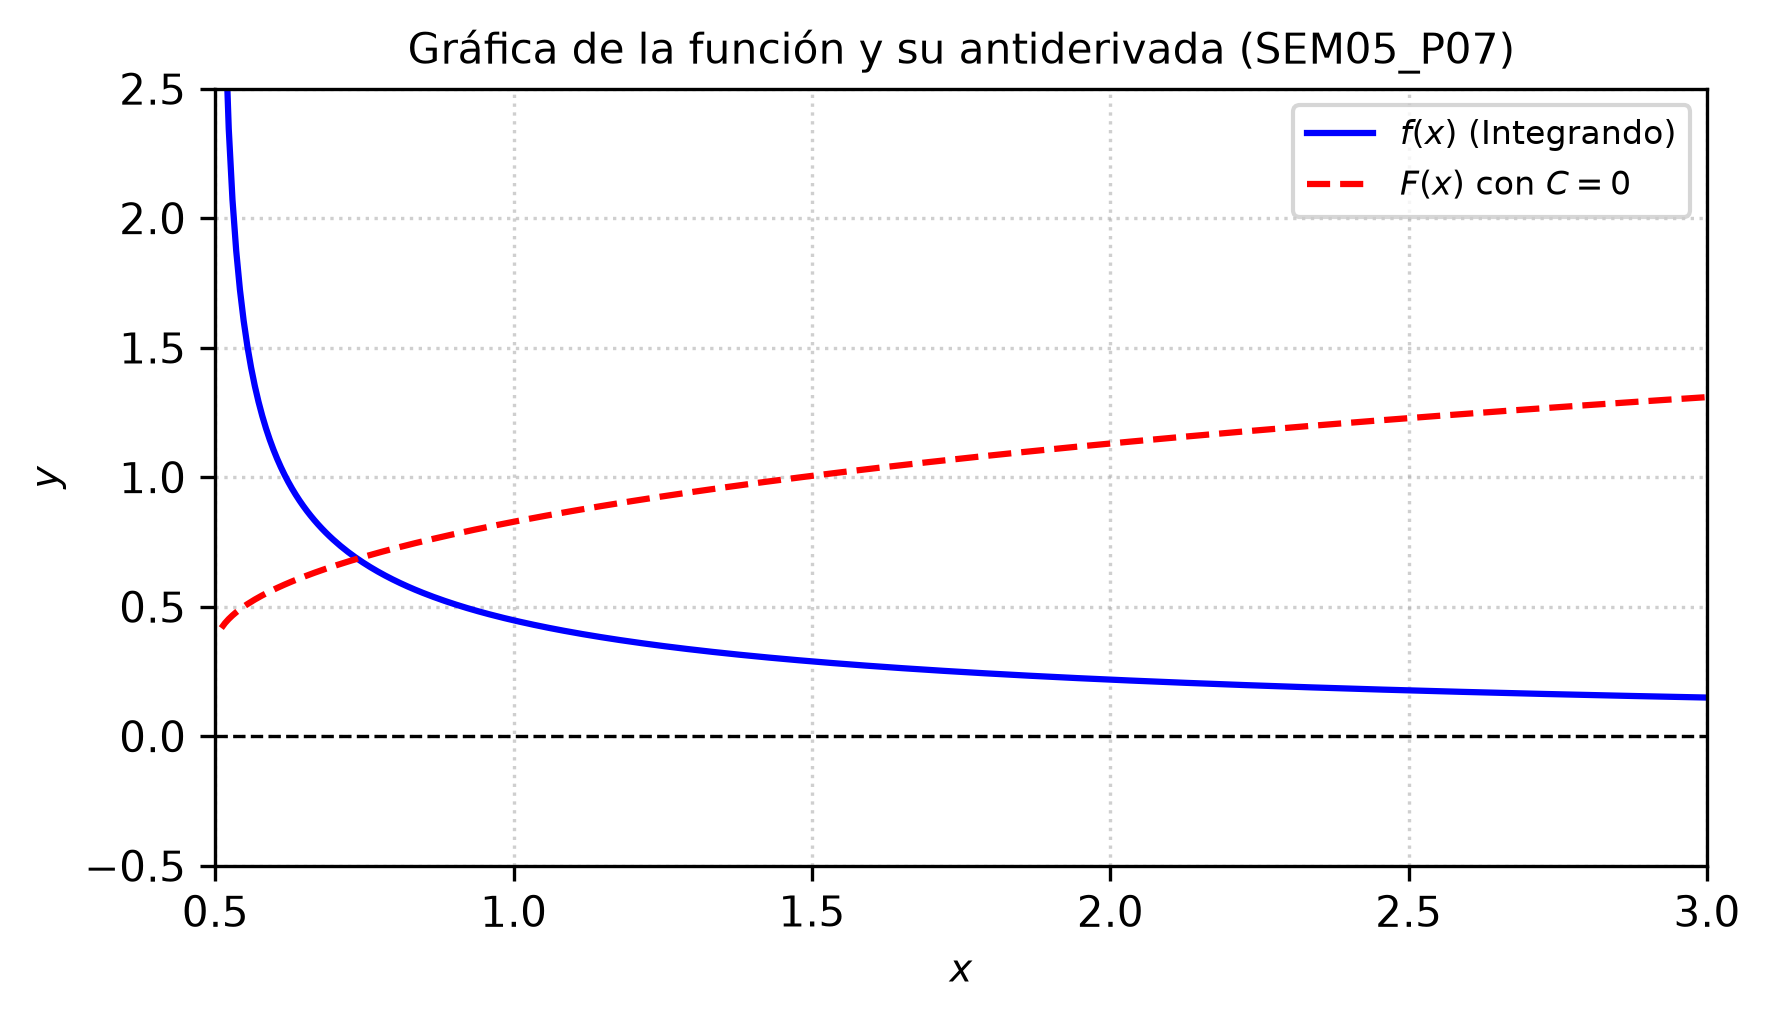
\includegraphics[width=\columnwidth]{semana_05/graficas/SEM05_P07_grafica.png}
	\caption{Representación gráfica de $f(x)$ y su antiderivada $F(x)$ evaluada para la constante de integración $C = 0$ (Problema 07).}
	\label{fig:problema07}
\end{figure}

	\subsection*{Problema 08}

\textbf{Enunciado:}
Calcular la integral indefinida:
\begin{align*}
\int \dfrac{dx}{\sqrt{x^2 + x + 1}}
\end{align*}

\textbf{Solución:}
Para resolver la integral, primero completamos el cuadrado en el trinomio del denominador:
\begin{align*}
x^2 + x + 1 &= \left(x + \dfrac{1}{2}\right)^2 \\
&\quad + 1 - \left(\dfrac{1}{2}\right)^2
\end{align*}

Simplificando los términos numéricos, obtenemos la expresión equivalente:
\begin{align*}
x^2 + x + 1 = \left(x + \dfrac{1}{2}\right)^2 + \dfrac{3}{4}
\end{align*}

Sustituimos esto en la integral original:
\begin{align*}
\int \dfrac{dx}{\sqrt{\left(x + \dfrac{1}{2}\right)^2 + \dfrac{3}{4}}}
\end{align*}

Utilizamos la fórmula de integración directa para funciones irracionales:
\begin{align*}
\int \dfrac{du}{\sqrt{u^2 + a^2}} = \ln\left|u + \sqrt{u^2 + a^2}\right| + C
\end{align*}

En nuestro caso, identificamos las variables:
\begin{align*}
u &= x + \dfrac{1}{2}, \quad dx = du \\
a^2 &= \dfrac{3}{4} \implies a = \dfrac{\sqrt{3}}{2}
\end{align*}

Aplicando la fórmula de integración, el resultado preliminar es:
\begin{align*}
\ln\left|x + \dfrac{1}{2} + \sqrt{x^2 + x + 1}\right| + C
\end{align*}

Por lo tanto, la solución general de la integral es:
\begin{align*}
\int \dfrac{dx}{\sqrt{x^2 + x + 1}} &= \ln\left|x + \dfrac{1}{2} \right. \\
&\quad \left. + \sqrt{x^2 + x + 1}\right| + C
\end{align*}

\begin{figure}[H]
	\centering
	
\includegraphics[width=\columnwidth]{semana_05/graficas/SEM05_P08_grafica.png}
	\caption{Representación gráfica de $f(x)$ y su antiderivada $F(x)$ evaluada para la constante de integración $C = 0$ (Problema 08).}
	\label{fig:problema08}
\end{figure}

	\subsection*{Problema 09}
\textbf{Enunciado:} Calcular la integral:
\begin{align*}
\int \sqrt{x^2 + x + 1} \, dx
\end{align*}

\textbf{Solución:} Primero completamos el cuadrado en el radicando:
\begin{align*}
x^2 + x + 1 &= \left(x^2 + x + \dfrac{1}{4}\right) + 1 - \dfrac{1}{4} \\
&= \left(x + \dfrac{1}{2}\right)^2 + \dfrac{3}{4}
\end{align*}

Sustituyendo esto en la integral, obtenemos:
\begin{align*}
\int \sqrt{\left(x + \dfrac{1}{2}\right)^2 + \dfrac{3}{4}} \, dx
\end{align*}

Utilizamos la sustitución trigonométrica:
\begin{align*}
x + \dfrac{1}{2} &= \dfrac{\sqrt{3}}{2} \tan\theta \\
dx &= \dfrac{\sqrt{3}}{2} \sec^2\theta \, d\theta
\end{align*}

El radicando se transforma en:
\begin{align*}
\sqrt{\left(\dfrac{\sqrt{3}}{2}\tan\theta\right)^2 + \dfrac{3}{4}} &= \sqrt{\dfrac{3}{4}(\tan^2\theta + 1)} \\
&= \dfrac{\sqrt{3}}{2} \sec\theta
\end{align*}

Sustituyendo $dx$ y el radical:
\begin{align*}
&= \int \left(\dfrac{\sqrt{3}}{2} \sec\theta\right) \left(\dfrac{\sqrt{3}}{2} \sec^2\theta \, d\theta\right) \\
&= \dfrac{3}{4} \int \sec^3\theta \, d\theta
\end{align*}

Usando la integral conocida de $\sec^3\theta$:
\begin{align*}
&= \dfrac{3}{8} \left( \sec\theta \tan\theta + \ln|\sec\theta + \tan\theta| \right) + C
\end{align*}

Regresando a la variable original $x$:
\begin{align*}
\tan\theta &= \dfrac{2x + 1}{\sqrt{3}}, \quad \sec\theta = \dfrac{2\sqrt{x^2 + x + 1}}{\sqrt{3}}
\end{align*}

Sustituyendo y simplificando, el resultado final es:
\begin{align*}
\int &\sqrt{x^2 + x + 1} \, dx = \dfrac{2x + 1}{4} \sqrt{x^2 + x + 1} \\
&+ \dfrac{3}{8} \ln\left| \dfrac{2\sqrt{x^2 + x + 1} + 2x + 1}{\sqrt{3}} \right| + C
\end{align*}

\begin{figure}[H]
	\centering
	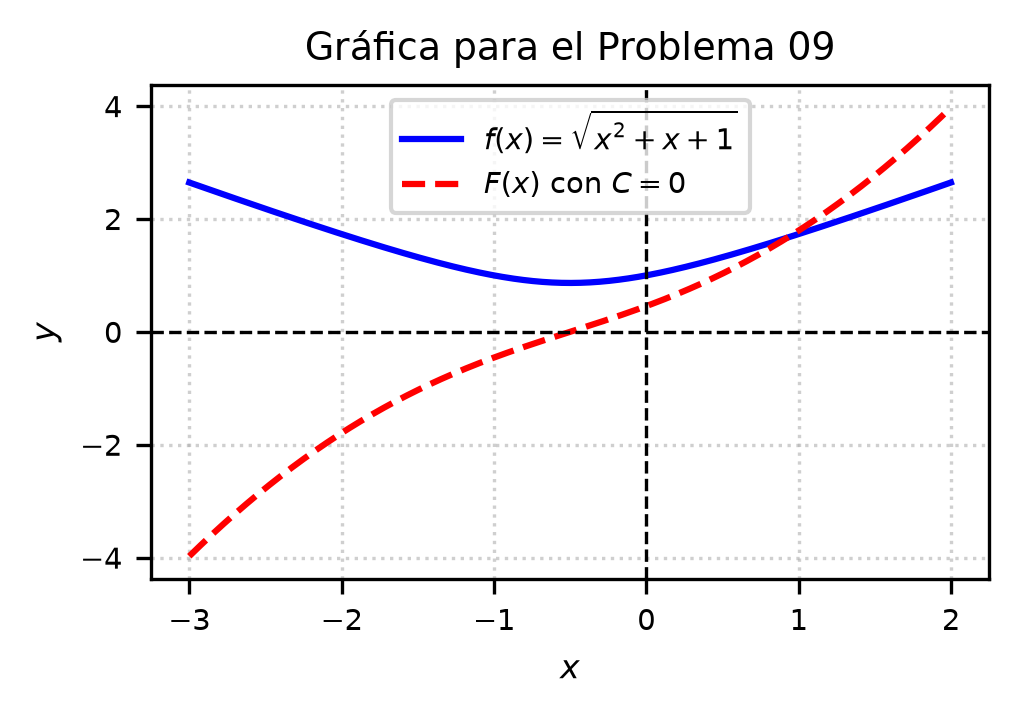
\includegraphics[width=\columnwidth]{semana_05/graficas/SEM05_P09_grafica.png}
	\caption{Representación gráfica de $f(x)$ y su antiderivada $F(x)$ evaluada para la constante de integración $C = 0$ (Problema 09).}
	\label{fig:problema09}
\end{figure}

	\subsection*{Problema 10}
\textbf{Enunciado:} Calcular la integral:
\begin{equation*}
\int \sqrt{x^2 + x + 1} \, dx
\end{equation*}

\textbf{Solución:} Para resolver la integral, comenzamos completando el cuadrado en el radicando:
\begin{align*}
x^2 + x + 1 &= \left(x^2 + x + \dfrac{1}{4}\right) + 1 - \dfrac{1}{4} \\
&= \left(x + \dfrac{1}{2}\right)^2 + \dfrac{3}{4}
\end{align*}

Sustituyendo esta expresión en la integral, obtenemos:
\begin{equation*}
\int \sqrt{\left(x + \dfrac{1}{2}\right)^2 + \dfrac{3}{4}} \, dx
\end{equation*}

Utilizamos la sustitución trigonométrica. 
Sea $x + \dfrac{1}{2} = \dfrac{\sqrt{3}}{2} \tan(\theta)$, de donde:
\begin{align*}
dx &= \dfrac{\sqrt{3}}{2} \sec^2(\theta) \, d\theta
\end{align*}

Además, la raíz cuadrada se transforma en:
\begin{align*}
\sqrt{\left(x + \dfrac{1}{2}\right)^2 + \dfrac{3}{4}} &= \sqrt{\dfrac{3}{4}\tan^2(\theta) + \dfrac{3}{4}} \\
&= \dfrac{\sqrt{3}}{2} \sec(\theta)
\end{align*}

Sustituyendo en la integral:
\begin{align*}
\int &\left(\dfrac{\sqrt{3}}{2} \sec(\theta)\right) \left(\dfrac{\sqrt{3}}{2} \sec^2(\theta)\right) d\theta \\
&= \dfrac{3}{4} \int \sec^3(\theta) \, d\theta
\end{align*}

Recordando la integral conocida de la secante cúbica:
\begin{align*}
\int \sec^3(\theta) \, d\theta &= \dfrac{1}{2} \sec(\theta) \tan(\theta) \\
&\quad + \dfrac{1}{2} \ln|\sec(\theta) + \tan(\theta)|
\end{align*}

Multiplicando por el factor $3/4$:
\begin{align*}
&= \dfrac{3}{8} \sec(\theta) \tan(\theta) \\
&\quad + \dfrac{3}{8} \ln|\sec(\theta) + \tan(\theta)| + C
\end{align*}

Volviendo a las variables originales con $\tan(\theta) = \dfrac{2x+1}{\sqrt{3}}$ y $\sec(\theta) = \dfrac{2\sqrt{x^2+x+1}}{\sqrt{3}}$:
\begin{align*}
&= \dfrac{2x+1}{4}\sqrt{x^2+x+1} \\
&\quad + \dfrac{3}{8}\ln\left| \dfrac{2\sqrt{x^2+x+1}}{\sqrt{3}} \right. \\
&\quad \left. + \dfrac{2x+1}{\sqrt{3}} \right| + C
\end{align*}

\begin{figure}[H]
	\centering
	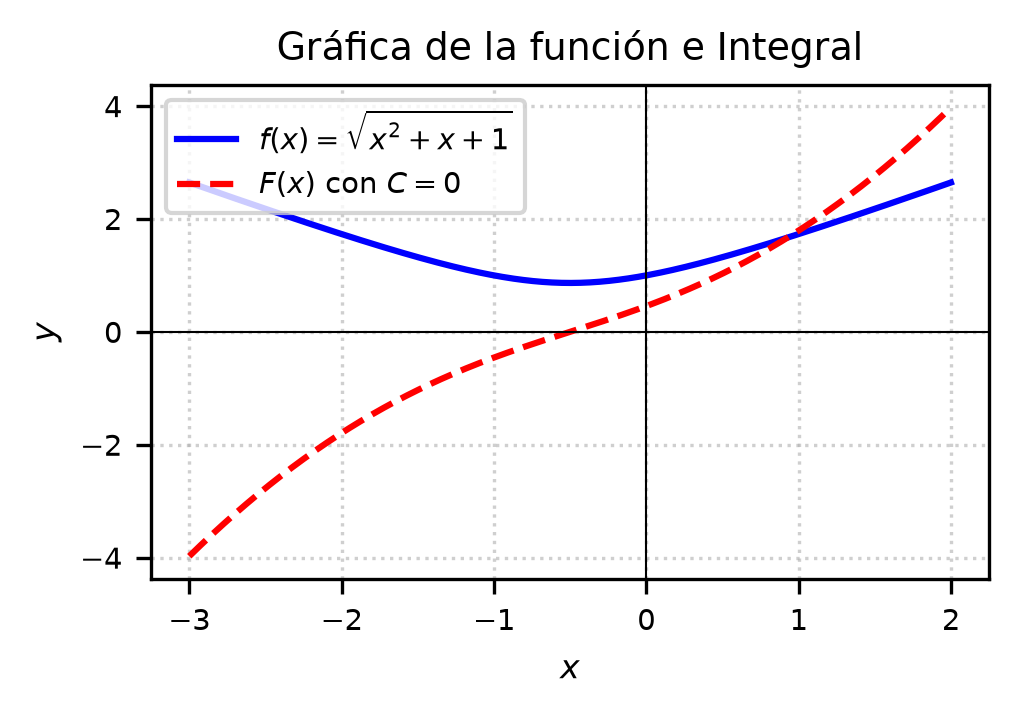
\includegraphics[width=\columnwidth]{semana_05/graficas/SEM05_P10_grafica.png}
	\caption{Representación gráfica de $f(x)$ y su antiderivada $F(x)$ evaluada para la constante de integración $C = 0$ (Problema 10).}
	\label{fig:problema10}
\end{figure}

	\subsection*{Problema 11}

\textbf{Enunciado:} \\
Calcular la integral indefinida:
\begin{align*}
I = \int \dfrac{x}{\sqrt{x^2 + 2x + 2}} \, dx
\end{align*}

\textbf{Solución:} \\
Para resolver esta integral, manipulamos el numerador para que aparezca la derivada del radicando, la cual es $2x + 2$. 

Escribimos el numerador como se indica:
\begin{align*}
x = \dfrac{1}{2}(2x + 2) - 1
\end{align*}

Sustituimos esta expresión en la integral original:
\begin{align*}
I &= \int \dfrac{\dfrac{1}{2}(2x + 2) - 1}{\sqrt{x^2 + 2x + 2}} \, dx
\end{align*}

Separamos la integral en dos partes:
\begin{align*}
I &= \dfrac{1}{2} \int \dfrac{2x + 2}{\sqrt{x^2 + 2x + 2}} \, dx \\
&\quad - \int \dfrac{1}{\sqrt{x^2 + 2x + 2}} \, dx
\end{align*}

Definimos $I_1$ para la primera integral y $I_2$ para la segunda, de modo que $I = \dfrac{1}{2}I_1 - I_2$.

Para $I_1$, hacemos el cambio de variable:
\begin{align*}
u &= x^2 + 2x + 2 \\
du &= (2x + 2) \, dx
\end{align*}

Sustituyendo en $I_1$:
\begin{align*}
I_1 &= \int \dfrac{du}{u^{1/2}} = \int u^{-1/2} \, du \\
&= 2u^{1/2} = 2\sqrt{x^2 + 2x + 2}
\end{align*}

Para $I_2$, completamos cuadrados en el denominador:
\begin{align*}
x^2 + 2x + 2 &= (x^2 + 2x + 1) + 1 \\
&= (x + 1)^2 + 1
\end{align*}

La segunda integral se convierte en:
\begin{align*}
I_2 &= \int \dfrac{dx}{\sqrt{(x+1)^2 + 1}}
\end{align*}

Utilizamos la fórmula de integración directa para funciones logarítmicas (o trigonométricas hiperbólicas):
\begin{align*}
I_2 &= \ln \left| (x+1) + \sqrt{(x+1)^2 + 1} \right| \\
&= \ln \left( x + 1 + \sqrt{x^2 + 2x + 2} \right)
\end{align*}

Finalmente, combinamos ambos resultados y agregamos la constante de integración $C$:
\begin{align*}
I &= \dfrac{1}{2} \left( 2\sqrt{x^2 + 2x + 2} \right) \\
&\quad - \ln \left( x + 1 + \sqrt{x^2 + 2x + 2} \right) + C
\end{align*}

Simplificando, obtenemos la solución final:
\begin{align*}
I &= \sqrt{x^2 + 2x + 2} \\
&\quad - \ln \left( x + 1 + \sqrt{x^2 + 2x + 2} \right) + C
\end{align*}

\begin{figure}[H]
	\centering
	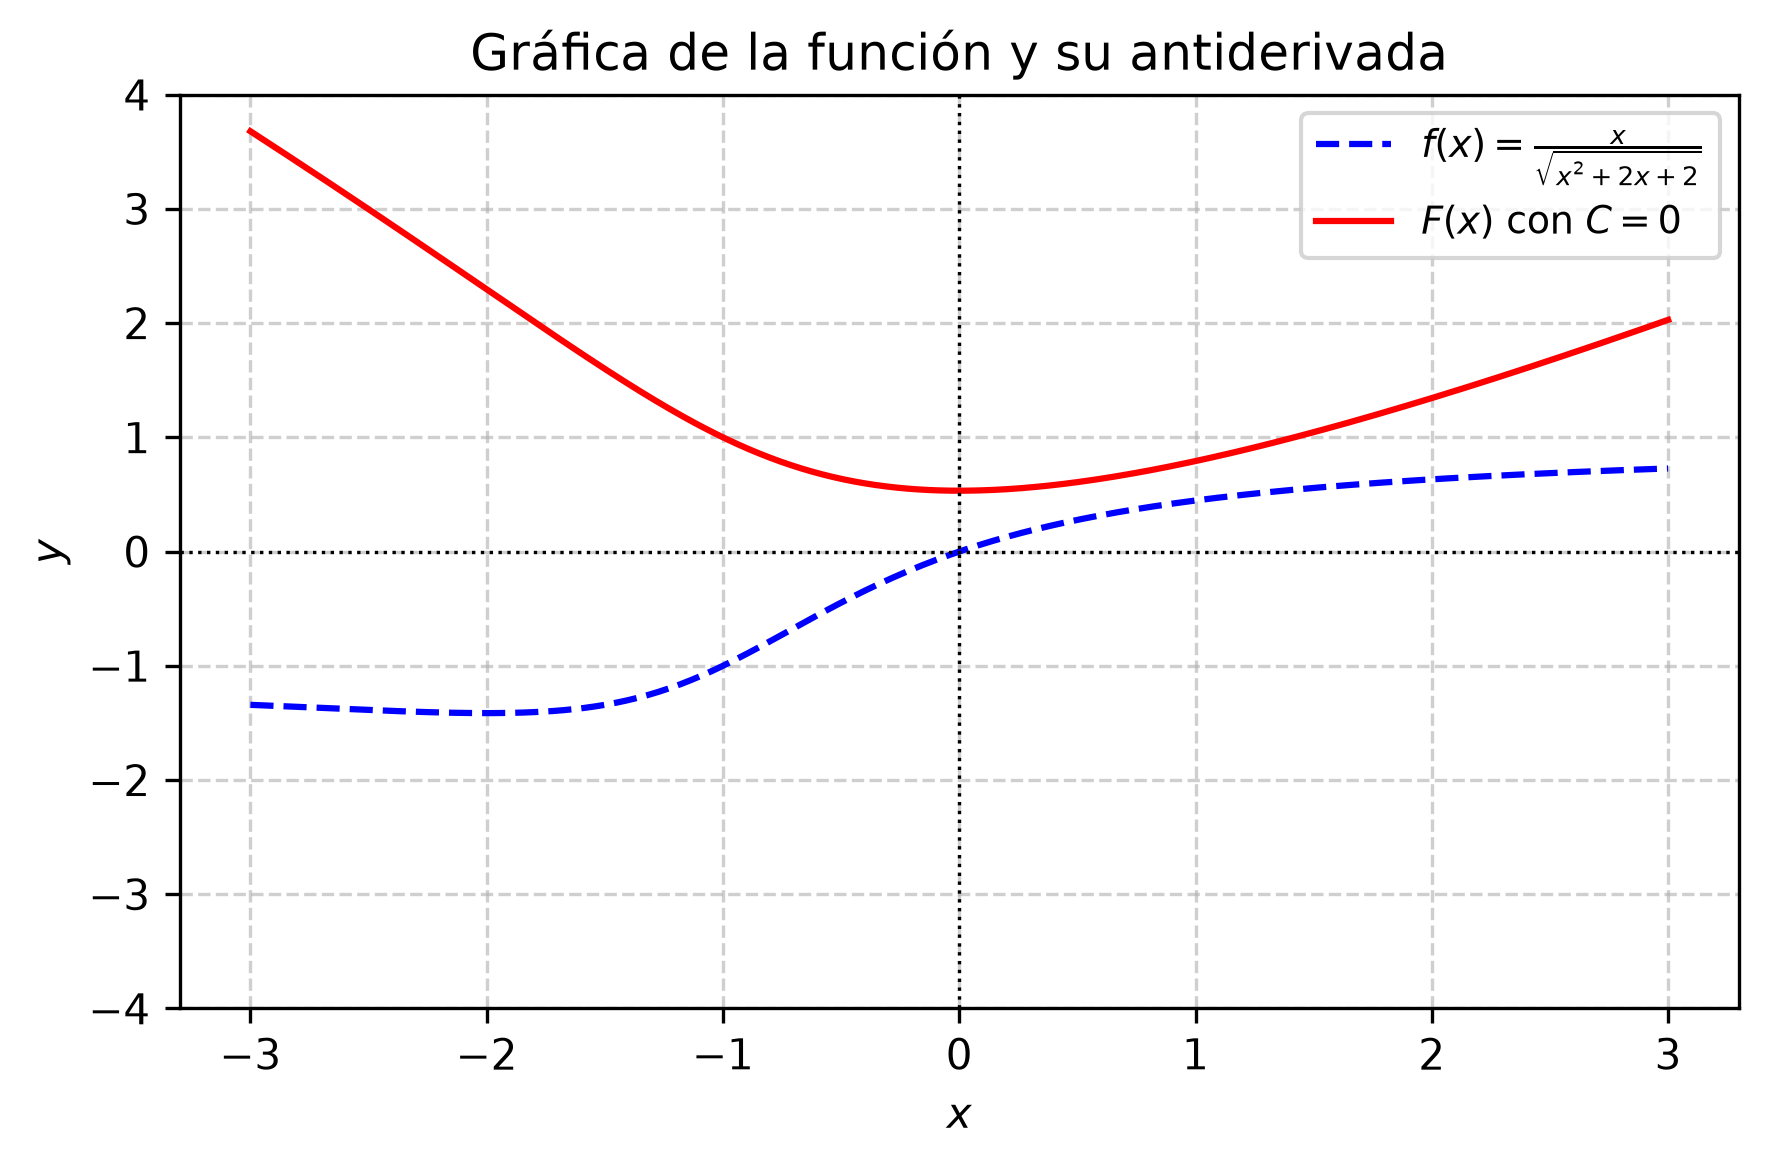
\includegraphics[width=\columnwidth]{semana_05/graficas/SEM05_P11_grafica.png}
	\caption{Representación gráfica de $f(x)$ y su antiderivada $F(x)$ evaluada para la constante de integración $C = 0$ (Problema 11).}
	\label{fig:problema11}
\end{figure}

	\subsection*{Problema 12}

\textbf{Enunciado:}
Calcular la integral indefinida:
\begin{equation*}
  \int \frac{x}{\sqrt{1 + x - x^2}} \, dx
\end{equation*}

\textbf{Solución:}
Siguiendo las indicaciones, reescribimos el numerador para que aparezca la derivada del argumento dentro de la raíz. 
Sea $u = 1 + x - x^2$, su derivada es $u' = 1 - 2x$. 
Modificamos el numerador del integrando:
\begin{align*}
  x &= -\frac{1}{2}(-2x) \\
  &= -\frac{1}{2}(1 - 2x - 1) \\
  &= -\frac{1}{2}(1 - 2x) + \frac{1}{2}
\end{align*}

Sustituimos esto en la integral original y separamos en dos partes:
\begin{align*}
  I &= \int \dfrac{-\frac{1}{2}(1 - 2x) + \frac{1}{2}}{\sqrt{1 + x - x^2}} \, dx \\
  &= -\frac{1}{2} \int \dfrac{1 - 2x}{\sqrt{1 + x - x^2}} \, dx \\
  &\quad + \frac{1}{2} \int \dfrac{1}{\sqrt{1 + x - x^2}} \, dx
\end{align*}

Para la primera integral, aplicamos sustitución directa con $u = 1 + x - x^2$ y $du = (1 - 2x) \, dx$:
\begin{align*}
  I_1 &= -\frac{1}{2} \int u^{-1/2} \, du \\
  &= -\frac{1}{2} \left( 2u^{1/2} \right) \\
  &= -\sqrt{1 + x - x^2}
\end{align*}

Para la segunda integral, completamos el cuadrado en el trinomio del denominador:
\begin{align*}
  1 + x - x^2 &= 1 - \left( x^2 - x \right) \\
  &= 1 - \left( x^2 - x + \frac{1}{4} - \frac{1}{4} \right) \\
  &= \frac{5}{4} - \left( x - \frac{1}{2} \right)^2
\end{align*}

Sustituimos esto en la segunda integral:
\begin{align*}
  I_2 &= \frac{1}{2} \int \dfrac{dx}{\sqrt{\left(\frac{\sqrt{5}}{2}\right)^2 - \left(x - \frac{1}{2}\right)^2}}
\end{align*}

Esta es una integral directa del tipo arcoseno:
\begin{align*}
  I_2 &= \frac{1}{2} \arcsin\left( \dfrac{x - \frac{1}{2}}{\frac{\sqrt{5}}{2}} \right) \\
  &= \frac{1}{2} \arcsin\left( \dfrac{2x - 1}{\sqrt{5}} \right)
\end{align*}

Finalmente, unimos ambos resultados y agregamos la constante de integración $C$:
\begin{align*}
  I &= -\sqrt{1 + x - x^2} \\
  &\quad + \frac{1}{2} \arcsin\left( \dfrac{2x - 1}{\sqrt{5}} \right) + C
\end{align*}

\begin{figure}[H]
	\centering
	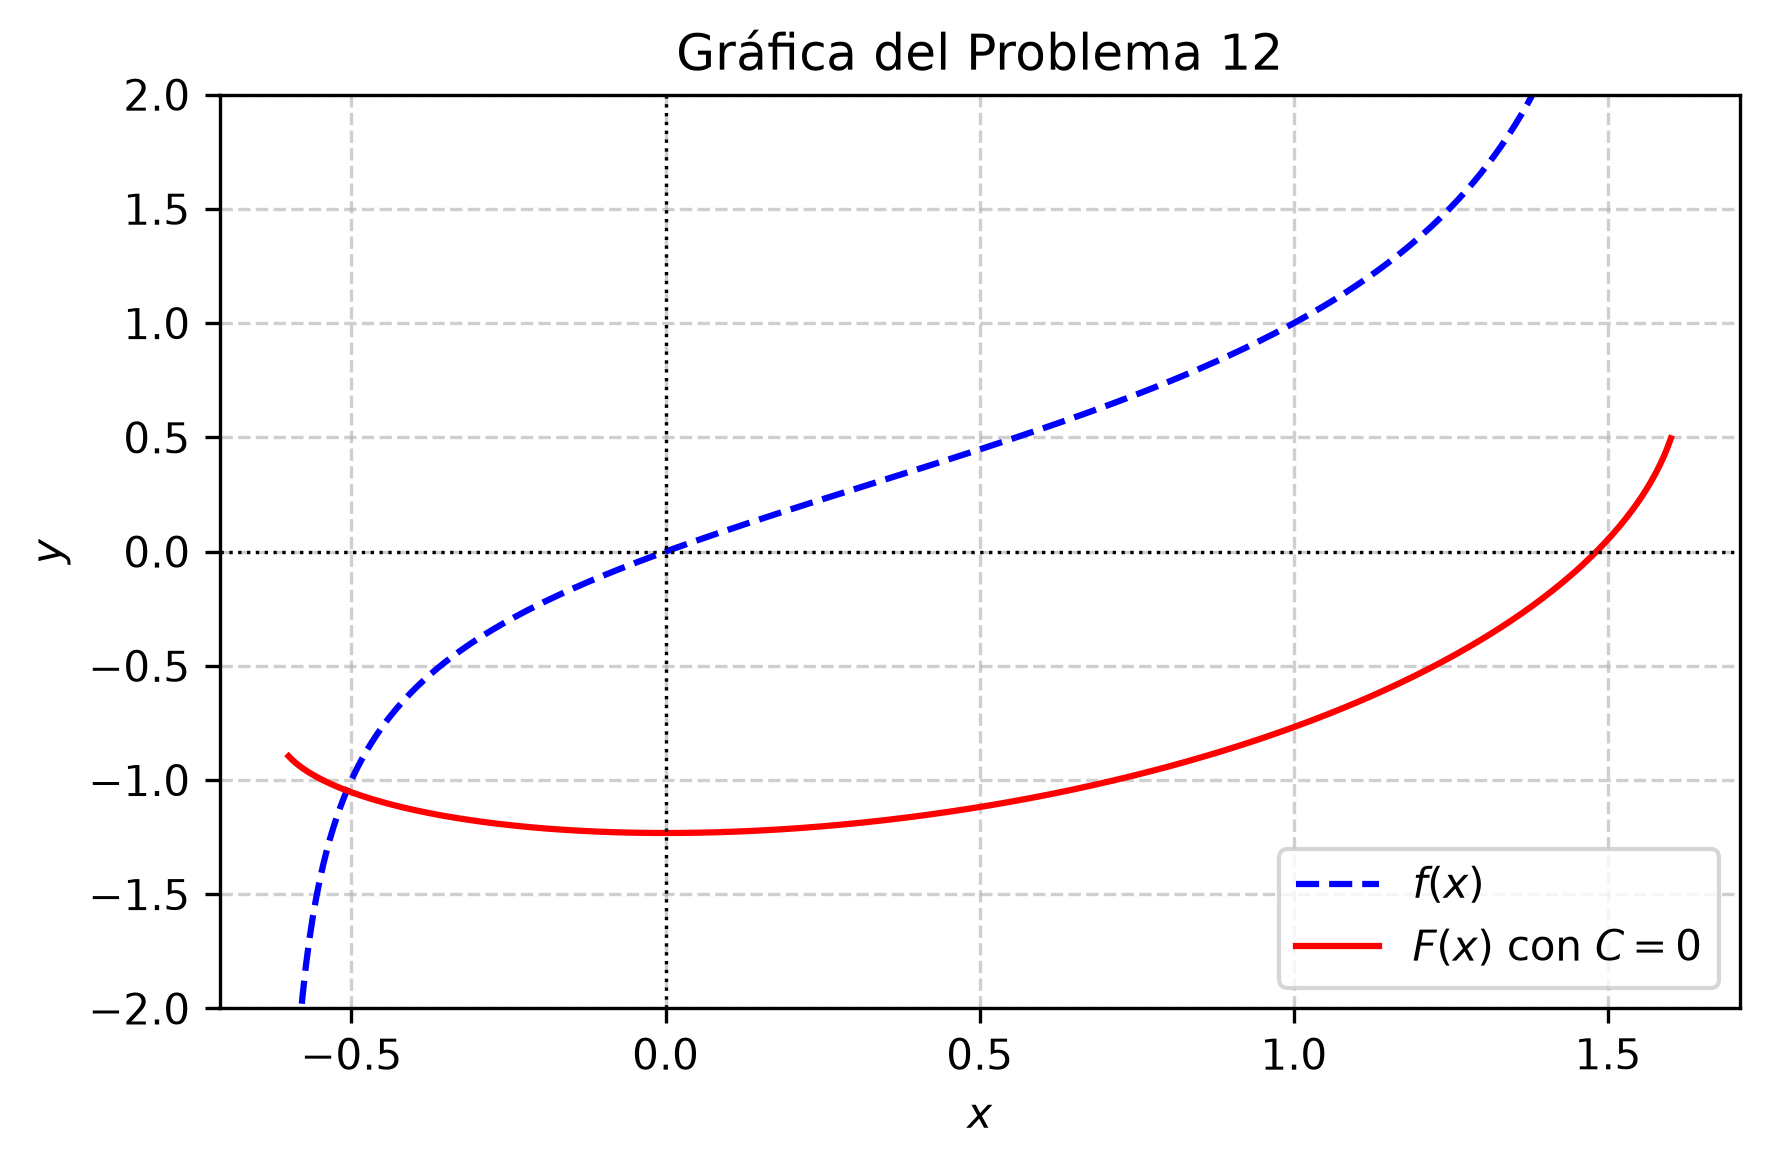
\includegraphics[width=\columnwidth]{semana_05/graficas/SEM05_P12_grafica.png}
	\caption{Representación gráfica de $f(x)$ y su antiderivada $F(x)$ evaluada para la constante de integración $C = 0$ (Problema 12).}
	\label{fig:problema12}
\end{figure}

	\subsection*{Problema 13}

\textbf{Enunciado:} 
Calcular la integral indefinida:
\begin{equation*}
\int \frac{1}{x \sqrt{1 + x - x^2}} \, dx
\end{equation*}

\textbf{Solución:} 
Para resolver la integral dada, aplicamos la 
sustitución recíproca sugerida, definiendo 
la nueva variable $u$ como:
\begin{equation*}
u = \frac{1}{x} \implies x = \frac{1}{u}
\end{equation*}

A partir de esta relación, el diferencial 
de $x$ se expresa como:
\begin{equation*}
dx = -\frac{1}{u^2} \, du
\end{equation*}

Sustituimos $x$ y $dx$ en la integral 
original. Notamos que $x$ en el denominador 
se convierte en $1/u$, y el término dentro 
del radical se transforma algebraicamente:
\begin{align*}
1 + x - x^2 &= 1 + \frac{1}{u} - \left(\frac{1}{u}\right)^2 \\
&= 1 + \frac{1}{u} - \frac{1}{u^2} \\
&= \frac{u^2 + u - 1}{u^2}
\end{align*}

Reemplazamos estos componentes 
dentro de la integral:
\begin{align*}
\int &\frac{1}{\left(\frac{1}{u}\right) 
\sqrt{\frac{u^2 + u - 1}{u^2}}} 
\left(-\frac{1}{u^2} \, du\right)
\end{align*}

Simplificamos la expresión algebraica 
factorizando el término $u^2$ del denominador 
dentro de la raíz cuadrada:
\begin{align*}
&= \int \frac{u}{\sqrt{\frac{u^2 + u - 1}{u^2}}} 
\left(-\frac{1}{u^2}\right) du \\
&= -\int \frac{u}{\left(\frac{\sqrt{u^2 + u - 1}}{u}\right)} 
\frac{1}{u^2} \, du \\
&= -\int \frac{u^2}{\sqrt{u^2 + u - 1}} 
\frac{1}{u^2} \, du \\
&= -\int \frac{1}{\sqrt{u^2 + u - 1}} \, du
\end{align*}

Para integrar esta función irracional, 
completamos el trinomio cuadrado 
dentro del radical:
\begin{align*}
u^2 + u - 1 &= \left(u^2 + u + \frac{1}{4}\right) 
- \frac{1}{4} - 1 \\
&= \left(u + \frac{1}{2}\right)^2 - \frac{5}{4}
\end{align*}

Sustituimos esta forma canónica en 
nuestra integral:
\begin{equation*}
-\int \frac{1}{\sqrt{\left(u + \frac{1}{2}\right)^2 
- \left(\frac{\sqrt{5}}{2}\right)^2}} \, du
\end{equation*}

Utilizamos la fórmula estándar de integración:
\begin{equation*}
\int \frac{dz}{\sqrt{z^2 - a^2}} = \ln \left| z + \sqrt{z^2 - a^2} \right|
\end{equation*}

Aplicando la fórmula con $z = u + \frac{1}{2}$ 
y $a = \frac{\sqrt{5}}{2}$:
\begin{align*}
-&\ln \left| \left(u + \frac{1}{2}\right) 
+ \sqrt{\left(u + \frac{1}{2}\right)^2 
- \left(\frac{\sqrt{5}}{2}\right)^2} \right| + C
\end{align*}

Reescribimos la expresión simplificando 
el radical a su forma original 
$u^2 + u - 1$:
\begin{equation*}
-\ln \left| u + \frac{1}{2} + \sqrt{u^2 + u - 1} \right| + C
\end{equation*}

Finalmente, regresamos a la variable 
original $x$ sustituyendo $u = \frac{1}{x}$:
\begin{align*}
-\ln &\left| \frac{1}{x} + \frac{1}{2} 
+ \sqrt{\frac{1}{x^2} + \frac{1}{x} - 1} \right| + C
\end{align*}

\begin{figure}[H]
	\centering
	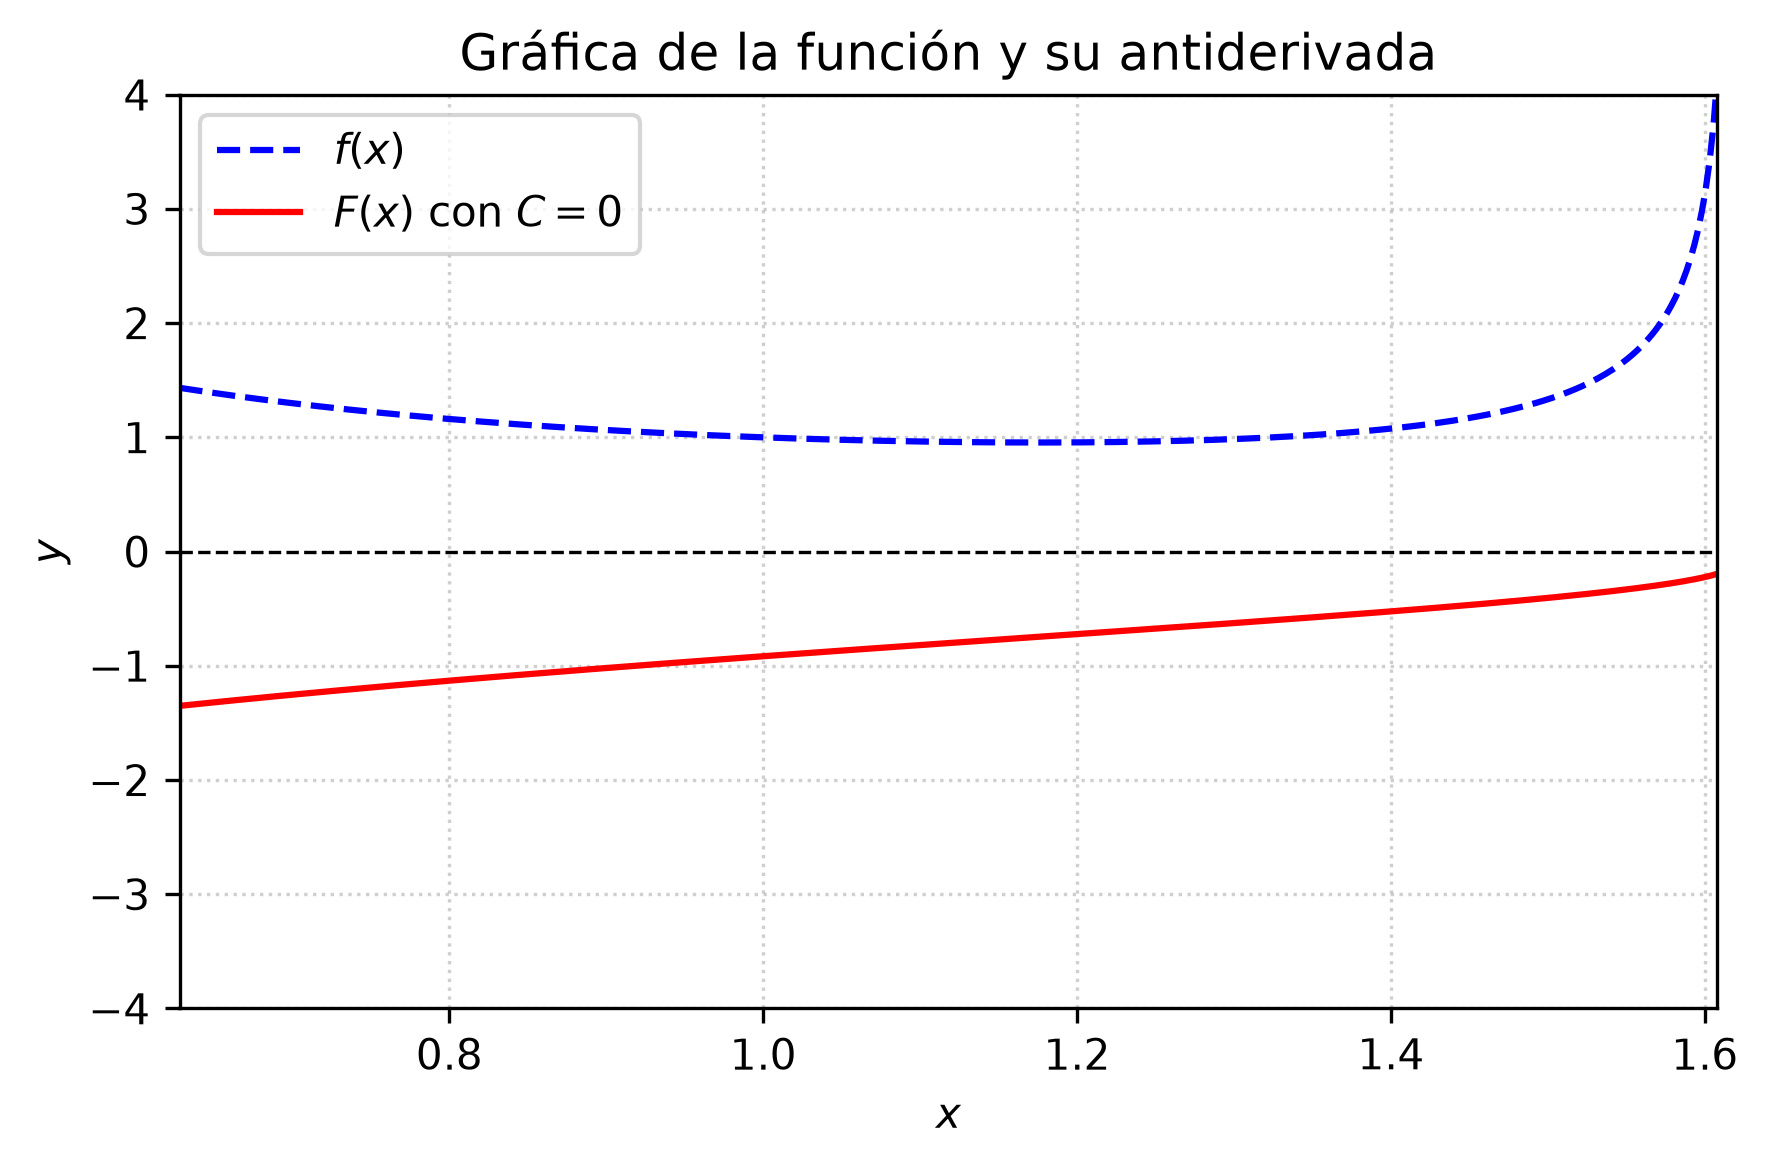
\includegraphics[width=\columnwidth]{semana_05/graficas/SEM05_P13_grafica.png}
	\caption{Representación gráfica de $f(x)$ y su antiderivada $F(x)$ evaluada para la constante de integración $C = 0$ (Problema 13).}
	\label{fig:problema13}
\end{figure}

	\subsection*{Problema 14}

\textbf{Enunciado:} Calcular la integral:
\begin{align*}
\int \dfrac{5x + 4}{\sqrt{x^2 + 2x + 5}} \, dx
\end{align*}

\textbf{Solución:} 
Primero, relacionamos la derivada del radicando $u = x^2 + 2x + 5$, cuya derivada es $du = (2x + 2) \, dx$. 

Expresamos el numerador en función de esta derivada según las indicaciones:
\begin{align*}
5x + 4 &= \dfrac{5}{2}(2x + 2) - 5 + 4 \\
&= \dfrac{5}{2}(2x + 2) - 1
\end{align*}

Sustituimos esto en la integral original y separamos en dos integrales:
\begin{align*}
I &= \int \dfrac{\frac{5}{2}(2x + 2) - 1}{\sqrt{x^2 + 2x + 5}} \, dx \\
I &= \dfrac{5}{2} \int \dfrac{2x + 2}{\sqrt{x^2 + 2x + 5}} \, dx \\
&\quad - \int \dfrac{1}{\sqrt{x^2 + 2x + 5}} \, dx
\end{align*}

Para la primera integral ($I_1$), usamos la sustitución $u = x^2 + 2x + 5$:
\begin{align*}
I_1 &= \dfrac{5}{2} \int u^{-1/2} \, du \\
&= \dfrac{5}{2} \left( 2u^{1/2} \right) = 5\sqrt{x^2 + 2x + 5}
\end{align*}

Para la segunda integral ($I_2$), completamos cuadrados en el denominador:
\begin{align*}
x^2 + 2x + 5 &= (x + 2x + 1) + 4 \\
&= (x + 1)^2 + 2^2
\end{align*}

Aplicando la fórmula de integración directa:
\begin{align*}
I_2 &= \int \dfrac{dx}{\sqrt{(x+1)^2 + 2^2}} \\
&= \ln\left| (x+1) + \sqrt{x^2 + 2x + 5} \right|
\end{align*}

Combinando ambos resultados y agregando la constante de integración $C$:
\begin{align*}
I &= 5\sqrt{x^2 + 2x + 5} \\
&\quad - \ln\left| x + 1 + \sqrt{x^2 + 2x + 5} \right| + C
\end{align*}

\begin{figure}[H]
	\centering
	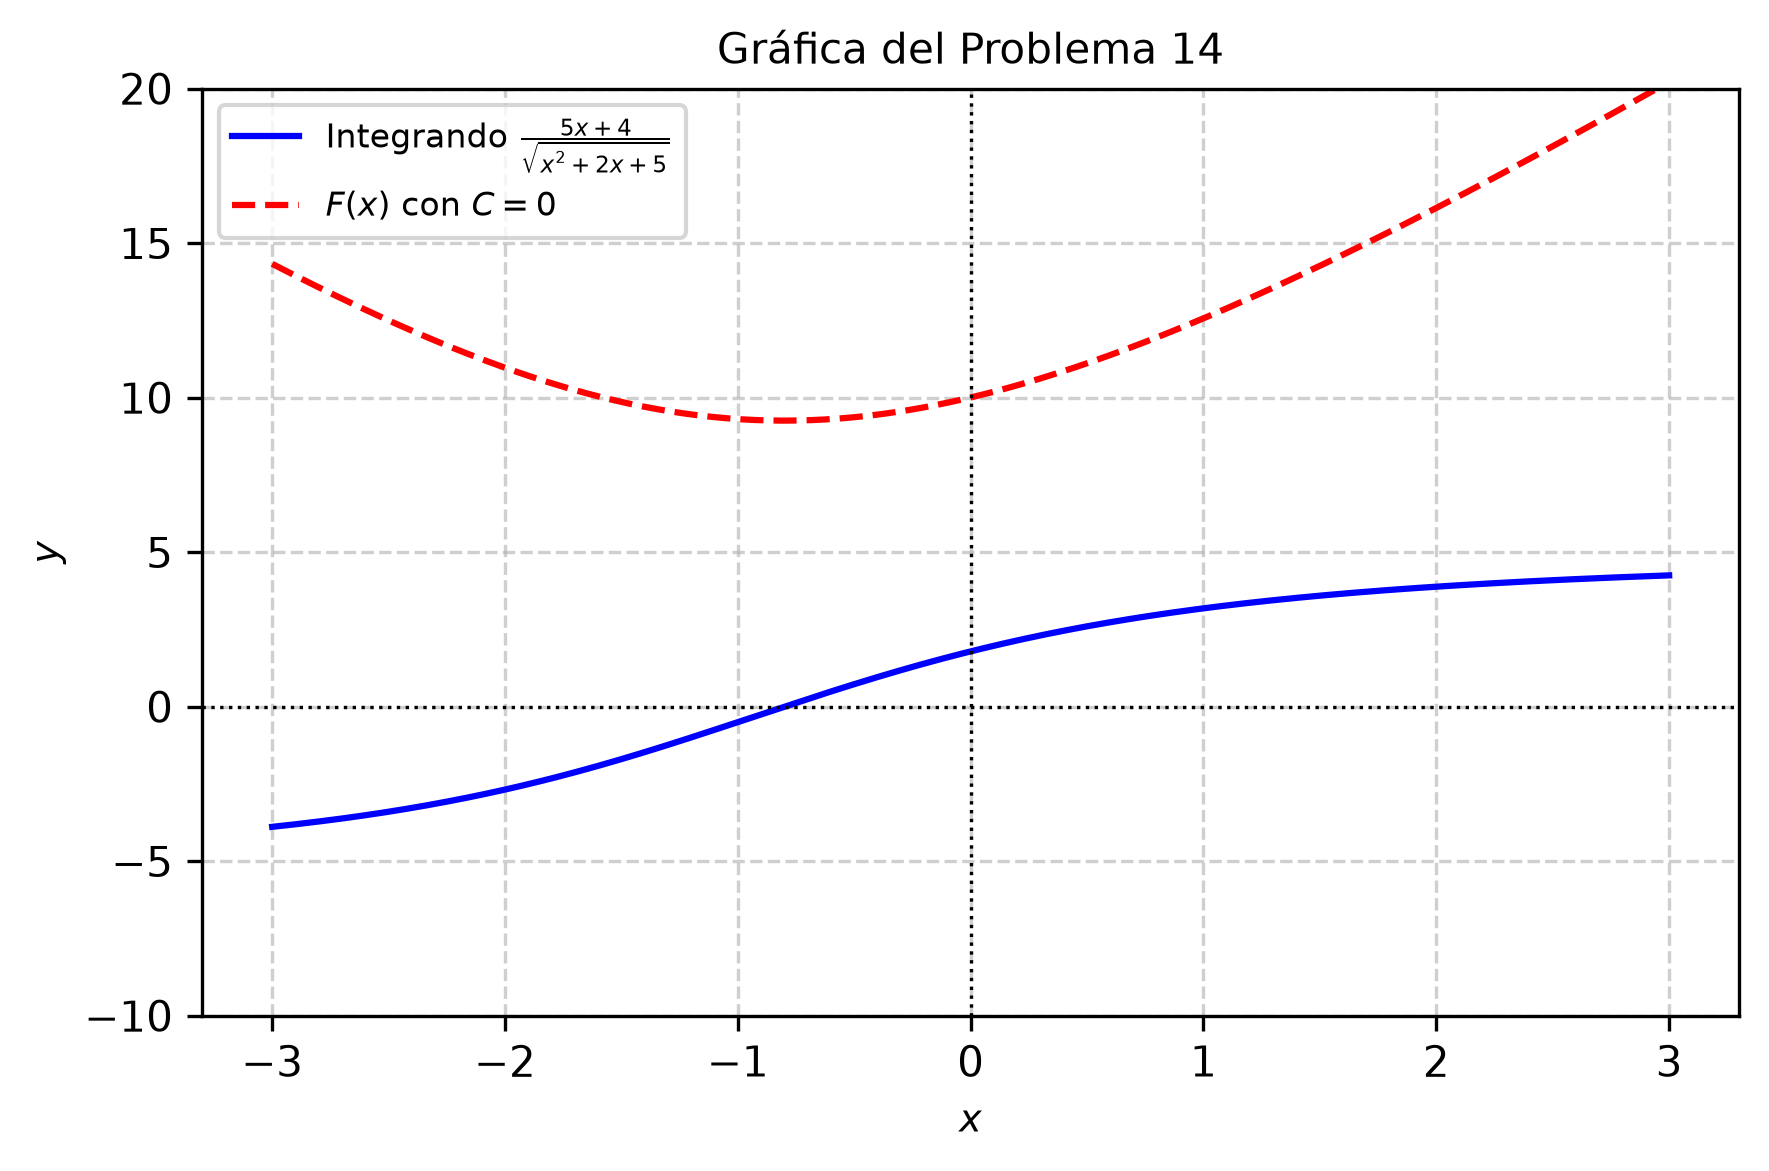
\includegraphics[width=\columnwidth]{semana_05/graficas/SEM05_P14_grafica.png}
	\caption{Representación gráfica de $f(x)$ y su antiderivada $F(x)$ evaluada para la constante de integración $C = 0$ (Problema 14).}
	\label{fig:problema14}
\end{figure}

	\subsection*{Problema 15}

\textbf{Enunciado:} \\
Calcular la integral:
\begin{align*}
\int \dfrac{x^3 - x^2 - 1}{\sqrt{x^2 + 2x + 2}} \, dx
\end{align*}

\textbf{Solución:} \\
Utilizamos el método de coeficientes indeterminados para integrales irracionales (método de Ostrogradski). Planteamos la forma de la solución:
\begin{align*}
\int &\dfrac{x^3 - x^2 - 1}{\sqrt{x^2 + 2x + 2}} \, dx = \\
&(Ax^2 + Bx + C)\sqrt{x^2 + 2x + 2} \\
&+ K \int \dfrac{dx}{\sqrt{x^2 + 2x + 2}}
\end{align*}

Derivamos ambos lados de la ecuación respecto a $x$ para eliminar el signo de integración:
\begin{align*}
\dfrac{x^3 - x^2 - 1}{\sqrt{x^2 + 2x + 2}} &= (2Ax + B)\sqrt{x^2 + 2x + 2} \\
&+ (Ax^2 + Bx + C)\dfrac{2x + 2}{2\sqrt{x^2 + 2x + 2}} \\
&+ \dfrac{K}{\sqrt{x^2 + 2x + 2}}
\end{align*}

Multiplicamos toda la expresión por $\sqrt{x^2 + 2x + 2}$ para simplificar los denominadores:
\begin{align*}
x^3 - x^2 - 1 &= (2Ax + B)(x^2 + 2x + 2) \\
&+ (Ax^2 + Bx + C)(x + 1) + K
\end{align*}

Expandimos los términos del lado derecho:
\begin{align*}
x^3 - x^2 - 1 &= 2Ax^3 + 4Ax^2 + 4Ax \\
&+ Bx^2 + 2Bx + 2B \\
&+ Ax^3 + Ax^2 + Bx^2 \\
&+ Bx + Cx + C + K
\end{align*}

Agrupamos los términos según las potencias de $x$:
\begin{align*}
x^3 - x^2 - 1 &= (3A)x^3 \\
&+ (5A + 2B)x^2 \\
&+ (4A + 3B + C)x \\
&+ (2B + C + K)
\end{align*}

Igualamos los coeficientes de ambos lados de la ecuación polinómica:
\begin{align*}
3A &= 1 \implies A = \dfrac{1}{3} \\
5A + 2B &= -1 \\
4A + 3B + C &= 0 \\
2B + C + K &= -1
\end{align*}

Sustituimos $A = 1/3$ en la segunda ecuación para hallar $B$:
\begin{align*}
5\left(\dfrac{1}{3}\right) + 2B &= -1 \implies 2B = -\dfrac{8}{3} \\
B &= -\dfrac{4}{3}
\end{align*}

Sustituimos $A$ y $B$ en la tercera ecuación para hallar $C$:
\begin{align*}
4\left(\dfrac{1}{3}\right) + 3\left(-\dfrac{4}{3}\right) + C &= 0 \\
\dfrac{4}{3} - 4 + C &= 0 \implies C = \dfrac{8}{3}
\end{align*}

Sustituimos $B$ y $C$ en la cuarta ecuación para hallar $K$:
\begin{align*}
2\left(-\dfrac{4}{3}\right) + \dfrac{8}{3} + K &= -1 \\
-\dfrac{8}{3} + \dfrac{8}{3} + K &= -1 \implies K = -1
\end{align*}

La integral resultante es:
\begin{align*}
\left(\dfrac{1}{3}x^2 - \dfrac{4}{3}x + \dfrac{8}{3}\right)&\sqrt{x^2 + 2x + 2} \\
&- \int \dfrac{dx}{\sqrt{x^2 + 2x + 2}}
\end{align*}

Completando el cuadrado para la integral restante:
\begin{align*}
\int \dfrac{dx}{\sqrt{(x+1)^2 + 1}} = \ln\left|x + 1 + \sqrt{x^2 + 2x + 2}\right|
\end{align*}

Finalmente, la solución general es:
\begin{align*}
\left(\dfrac{x^2 - 4x + 8}{3}\right)&\sqrt{x^2 + 2x + 2} \\
&- \ln\left|x + 1 + \sqrt{x^2 + 2x + 2}\right| + C
\end{align*}

\begin{figure}[H]
	\centering
	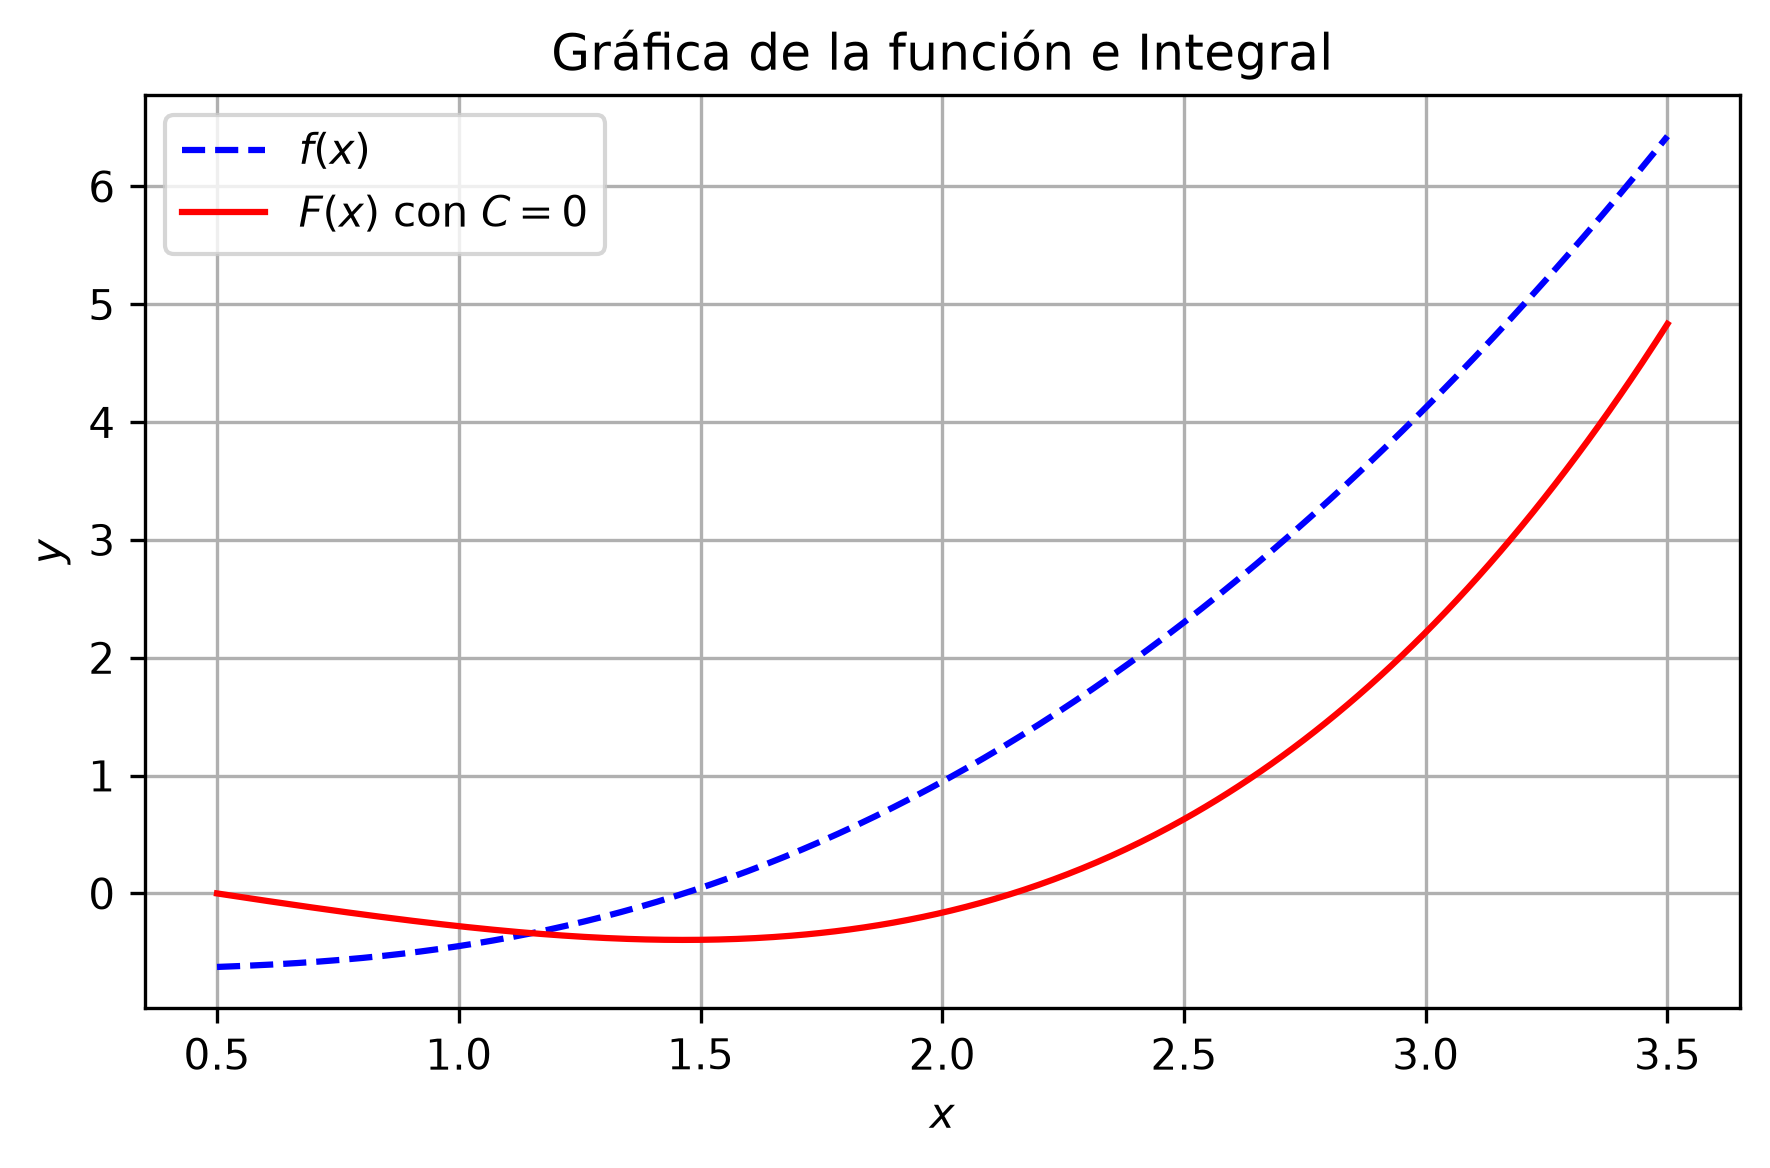
\includegraphics[width=\columnwidth]{semana_05/graficas/SEM05_P15_grafica.png}
	\caption{Representación gráfica de $f(x)$ y su antiderivada $F(x)$ evaluada para la constante de integración $C = 0$ (Problema 15).}
	\label{fig:problema15}
\end{figure}

	\subsection*{Problema 16}
\textbf{Enunciado:} Calcular la integral:
\begin{equation*}
\int \frac{9x^3 - 3x^2 + 2}{\sqrt{3x^2 - 2x + 1}} \, dx
\end{equation*}

\textbf{Solución:} Para resolver integrales de la forma $\int \frac{P_n(x)}{\sqrt{ax^2+bx+c}} \, dx$, empleamos el método de coeficientes indeterminados. Proponemos la identidad:
\begin{align*}
\int &\frac{9x^3 - 3x^2 + 2}{\sqrt{3x^2 - 2x + 1}} \, dx = \\
&(Ax^2 + Bx + C)\sqrt{3x^2 - 2x + 1} \\
&+ K \int \frac{dx}{\sqrt{3x^2 - 2x + 1}}
\end{align*}

Derivamos ambos miembros de la ecuación respecto a $x$:
\begin{align*}
\frac{9x^3 - 3x^2 + 2}{\sqrt{3x^2 - 2x + 1}} &= (2Ax + B)\sqrt{3x^2 - 2x + 1} \\
&+ (Ax^2 + Bx + C)\frac{6x - 2}{2\sqrt{3x^2 - 2x + 1}} \\
&+ \frac{K}{\sqrt{3x^2 - 2x + 1}}
\end{align*}

Multiplicamos toda la expresión por $\sqrt{3x^2 - 2x + 1}$ para eliminar denominadores:
\begin{align*}
9x^3 &- 3x^2 + 2 = (2Ax + B)(3x^2 - 2x + 1) \\
&+ (Ax^2 + Bx + C)(3x - 1) + K
\end{align*}

Desarrollamos los productos del lado derecho:
\begin{align*}
9x^3 &- 3x^2 + 2 = (6x^3 - 4x^2 + 2Ax \\
&+ 3Bx^2 - 2Bx + B) + (3Ax^3 \\
&- Ax^2 + 3Bx^2 - Bx + 3Cx - C) + K
\end{align*}

Agrupamos los términos según las potencias de $x$:
\begin{align*}
9x^3 &- 3x^2 + 2 = 9Ax^3 \\
&+ (-4A + 6B - A)x^2 \\
&+ (2A - 2B - B + 3C)x \\
&+ (B - C + K)
\end{align*}

Simplificamos los coeficientes:
\begin{align*}
9x^3 &- 3x^2 + 2 = 9Ax^3 \\
&+ (-5A + 6B)x^2 \\
&+ (2A - 3B + 3C)x \\
&+ (B - C + K)
\end{align*}

Igualamos los coeficientes de potencias homólogas:
\begin{align*}
x^3: &\quad 9A = 9 \implies A = 1 \\
x^2: &\quad -5A + 6B = -3 \\
x^1: &\quad 2A - 3B + 3C = 0 \\
x^0: &\quad B - C + K = 2
\end{align*}

Resolviendo el sistema de ecuaciones:
\begin{align*}
-5(1) + 6B &= -3 \implies 6B = 2 \implies B = \dfrac{1}{3} \\
2(1) &- 3\left(\dfrac{1}{3}\right) + 3C = 0 \implies 1 + 3C = 0 \implies C = -\dfrac{1}{3} \\
\dfrac{1}{3} &- \left(-\dfrac{1}{3}\right) + K = 2 \implies \dfrac{2}{3} + K = 2 \implies K = \dfrac{4}{3}
\end{align*}

Sustituimos los valores en la solución propuesta:
\begin{align*}
\int &\frac{9x^3 - 3x^2 + 2}{\sqrt{3x^2 - 2x + 1}} \, dx = \left(x^2 + \dfrac{1}{3}x - \dfrac{1}{3}\right)\sqrt{3x^2 - 2x + 1} \\
&+ \dfrac{4}{3} \int \frac{dx}{\sqrt{3x^2 - 2x + 1}}
\end{align*}

Completamos el trinomio cuadrado perfecto:
\begin{align*}
3x^2 - 2x + 1 &= 3\left(x^2 - \dfrac{2}{3}x + \dfrac{1}{3}\right) \\
&= 3\left[\left(x - \dfrac{1}{3}\right)^2 + \dfrac{2}{9}\right]
\end{align*}

La integral restante se resuelve mediante sustitución trigonométrica o fórmula directa:
\begin{align*}
\int &\frac{dx}{\sqrt{3\left(x - \frac{1}{3}\right)^2 + \frac{2}{3}}} = \dfrac{1}{\sqrt{3}} \ln\left|u + \sqrt{u^2 + a^2}\right|
\end{align*}
donde $u = x - \frac{1}{3}$ y $a^2 = \frac{2}{9}$.

Finalmente, la solución general es:
\begin{align*}
&= \left(x^2 + \dfrac{1}{3}x - \dfrac{1}{3}\right)\sqrt{3x^2 - 2x + 1} \\
&+ \dfrac{4}{3\sqrt{3}} \ln\left|x - \dfrac{1}{3} + \sqrt{x^2 - \dfrac{2}{3}x + \dfrac{1}{3}}\right| + C
\end{align*}

\begin{figure}[H]
	\centering
	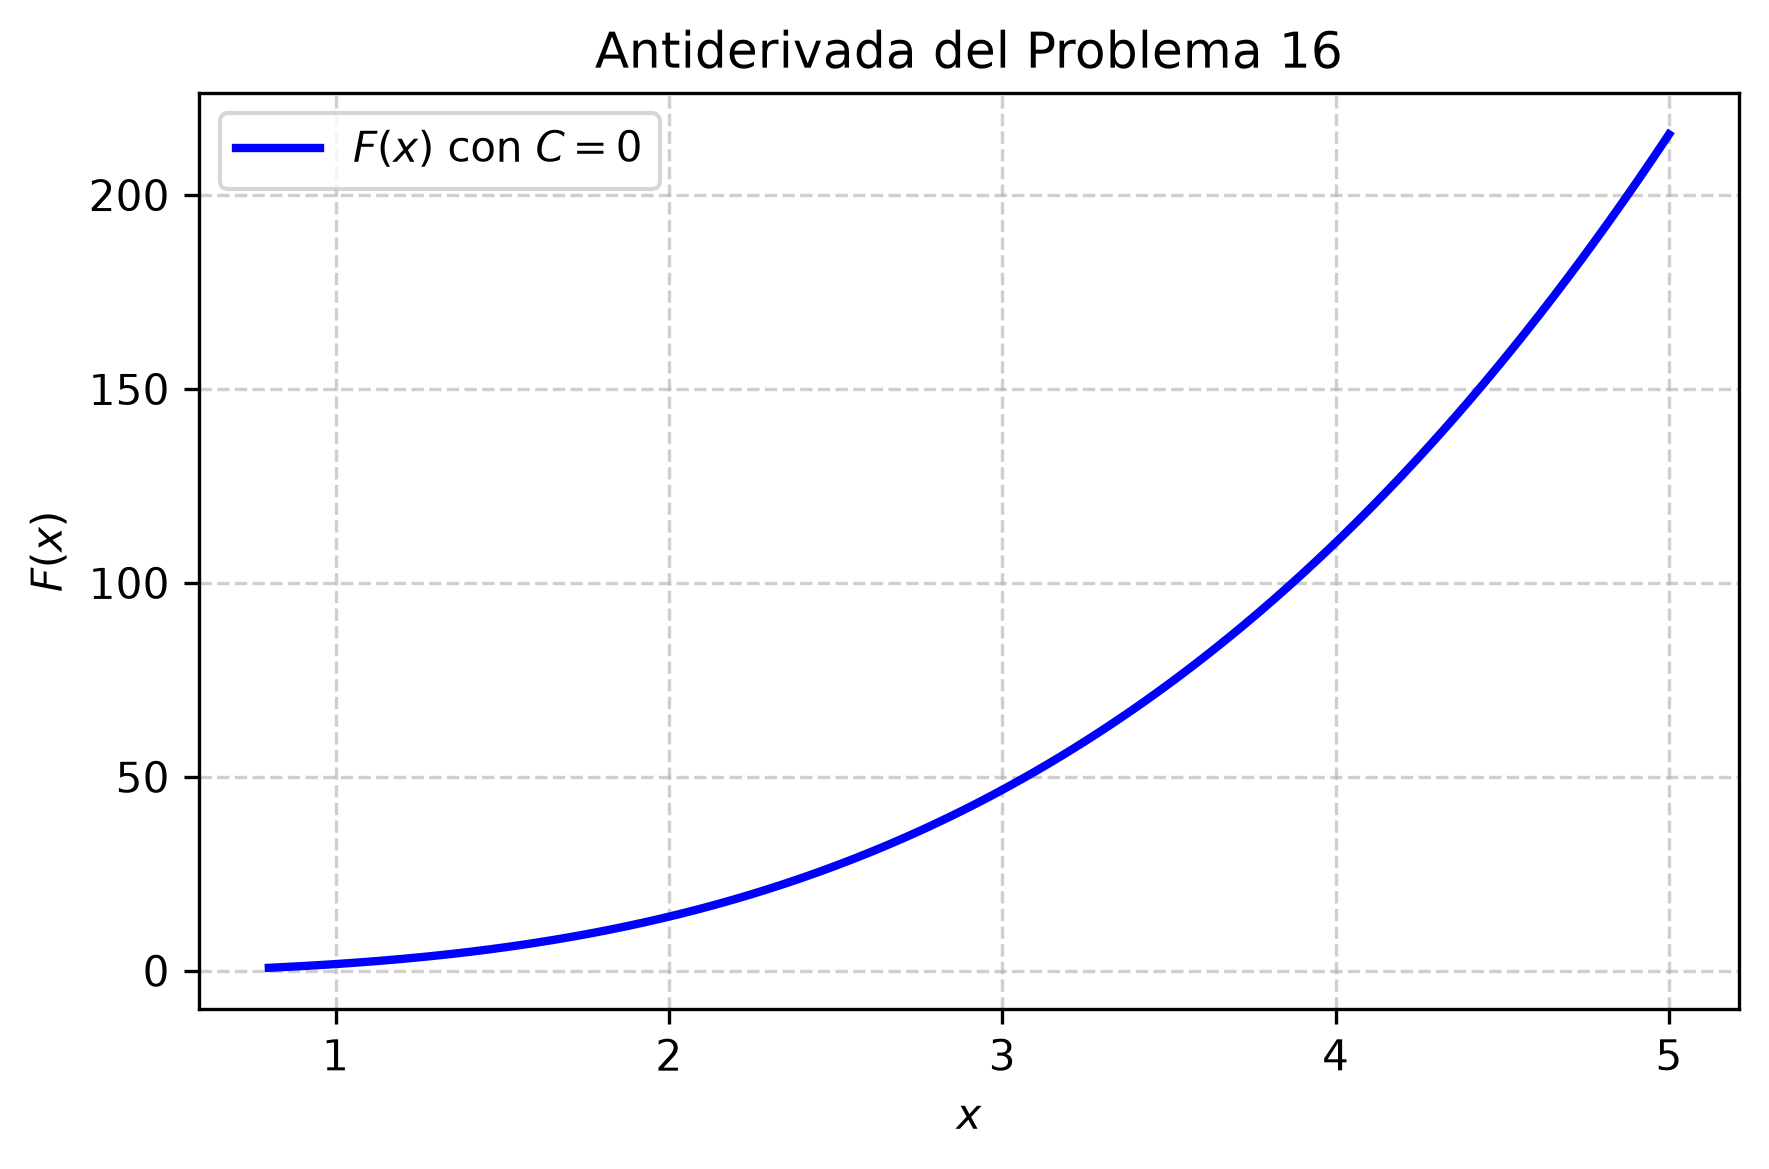
\includegraphics[width=\columnwidth]{semana_05/graficas/SEM05_P16_grafica.png}
	\caption{Representación gráfica de $f(x)$ y su antiderivada $F(x)$ evaluada para la constante de integración $C = 0$ (Problema 16).}
	\label{fig:problema16}
\end{figure}

	\subsection*{Problema 17}

\textbf{Enunciado:}
Calcular la integral indefinida:
\begin{align*}
\int \sqrt{x^2 + x + 1} \, dx
\end{align*}

\textbf{Solución:}
Para resolver la integral, primero completamos el trinomio cuadrado perfecto dentro del radical:
\begin{align*}
x^2 + x + 1 &= \left(x + \dfrac{1}{2}\right)^2 + \dfrac{3}{4}
\end{align*}

Sustituyendo esto en la integral:
\begin{align*}
I &= \int \sqrt{\left(x + \dfrac{1}{2}\right)^2 + \dfrac{3}{4}} \, dx
\end{align*}

Aplicamos la sustitución trigonométrica recomendada:
\begin{align*}
x + \dfrac{1}{2} &= \dfrac{\sqrt{3}}{2} \tan\theta \\
dx &= \dfrac{\sqrt{3}}{2} \sec^2\theta \, d\theta
\end{align*}

El término dentro de la raíz se transforma en:
\begin{align*}
\sqrt{\left(x + \dfrac{1}{2}\right)^2 + \dfrac{3}{4}} &= \sqrt{\dfrac{3}{4}\tan^2\theta + \dfrac{3}{4}} \\
&= \dfrac{\sqrt{3}}{2} \sec\theta
\end{align*}

Sustituyendo en la integral en términos de $\theta$:
\begin{align*}
I &= \int \left(\dfrac{\sqrt{3}}{2}\sec\theta\right) \left(\dfrac{\sqrt{3}}{2}\sec^2\theta \, d\theta\right) \\
&= \dfrac{3}{4} \int \sec^3\theta \, d\theta
\end{align*}

Utilizando la conocida integral de la secante cubica:
\begin{align*}
\int \sec^3\theta \, d\theta &= \dfrac{1}{2} \sec\theta \tan\theta \\
&\quad + \dfrac{1}{2} \ln|\sec\theta + \tan\theta|
\end{align*}

Regresando a la variable original $x$, recordamos que $\tan\theta = \dfrac{2x+1}{\sqrt{3}}$ y $\sec\theta = \dfrac{2\sqrt{x^2+x+1}}{\sqrt{3}}$. Sustituyendo y simplificando:
\begin{align*}
I &= \dfrac{2x+1}{4}\sqrt{x^2+x+1} \\
&\quad + \dfrac{3}{8}\ln\left|\dfrac{2\sqrt{x^2+x+1}}{\sqrt{3}} + \dfrac{2x+1}{\sqrt{3}}\right| + C
\end{align*}

\begin{figure}[H]
	\centering
	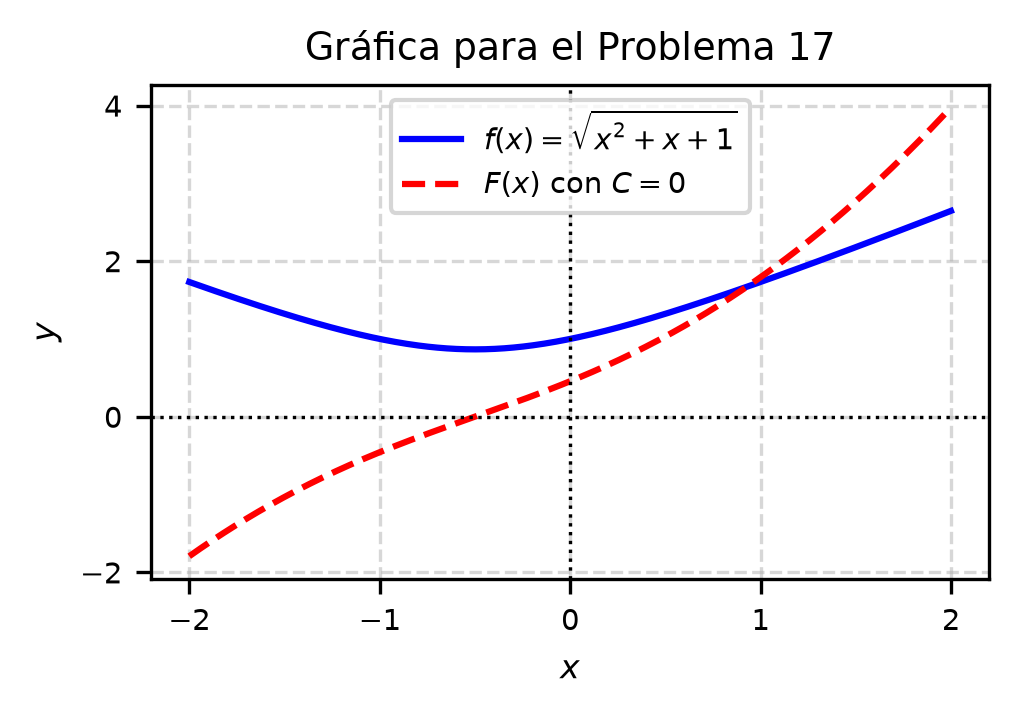
\includegraphics[width=\columnwidth]{semana_05/graficas/SEM05_P17_grafica.png}
	\caption{Representación gráfica de $f(x)$ y su antiderivada $F(x)$ evaluada para la constante de integración $C = 0$ (Problema 17).}
	\label{fig:problema17}
\end{figure}

	\subsection*{Problema 18}

Calcule la siguiente integral indefinida:
\begin{align*}
I = \int \sqrt{x^2 + 2x + 2} \, dx
\end{align*}

\textbf{Solución:}

Primero, completamos el cuadrado dentro
del radicando de la función:
\begin{align*}
x^2 + 2x + 2 &= (x^2 + 2x + 1) + 1 \\
&= (x + 1)^2 + 1
\end{align*}

Sustituimos esto en la integral original:
\begin{align*}
I = \int \sqrt{(x + 1)^2 + 1} \, dx
\end{align*}

Aplicamos el método de sustitución
trigonométrica. Sea:
\begin{align*}
x + 1 &= \tan\theta \\
dx &= \sec^2\theta \, d\theta
\end{align*}

Sustituimos en la integral:
\begin{align*}
I &= \int \sqrt{\tan^2\theta + 1} \, (\sec^2\theta \, d\theta)
\end{align*}

Utilizamos la identidad trigonométrica
$\tan^2\theta + 1 = \sec^2\theta$:
\begin{align*}
I &= \int \sqrt{\sec^2\theta} \sec^2\theta \, d\theta \\
&= \int \sec^3\theta \, d\theta
\end{align*}

La integral de la secante al cubo es
una integral estándar que se resuelve por
partes:
\begin{align*}
\int \sec^3\theta \, d\theta = \dfrac{1}{2} \sec\theta \tan\theta \\
+ \dfrac{1}{2} \ln|\sec\theta + \tan\theta| + C
\end{align*}

Devolvemos las variables a términos de $x$.
Sabemos que $\tan\theta = x + 1$.
Por trigonometría en un triángulo rectángulo:
\begin{align*}
\tan\theta &= \dfrac{x + 1}{1} \\
\sec\theta &= \sqrt{(x + 1)^2 + 1} \\
&= \sqrt{x^2 + 2x + 2}
\end{align*}

Sustituimos estas expresiones en el
resultado:
\begin{align*}
I &= \dfrac{1}{2} (x + 1)\sqrt{x^2 + 2x + 2} \\
&\quad + \dfrac{1}{2} \ln \left| \sqrt{x^2 + 2x + 2} \right. \\
&\quad \left. + x + 1 \right| + C
\end{align*}

Por lo tanto, la solución general es:
\begin{align*}
I &= \dfrac{x + 1}{2} \sqrt{x^2 + 2x + 2} \\
&\quad + \dfrac{1}{2} \ln \left( x + 1 \right. \\
&\quad \left. + \sqrt{x^2 + 2x + 2} \right) + C
\end{align*}

\begin{figure}[H]
	\centering
	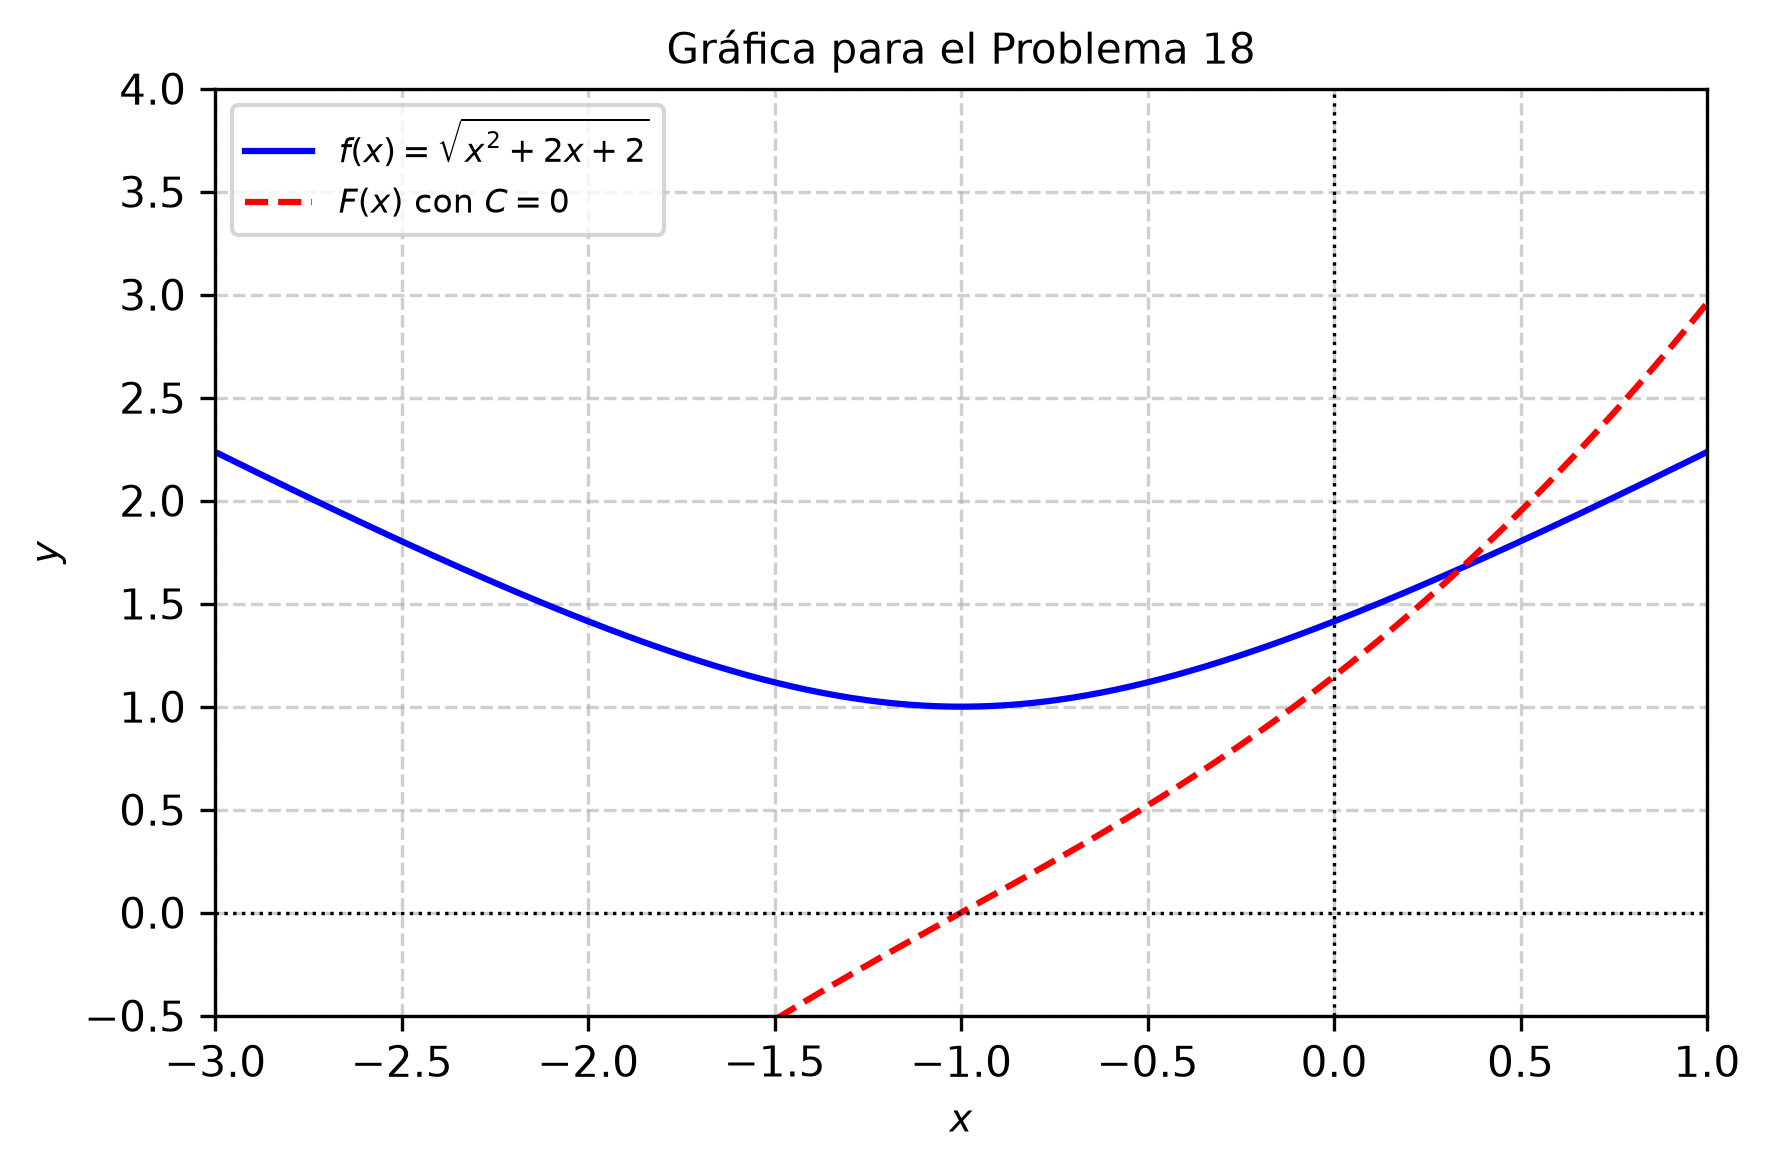
\includegraphics[width=\columnwidth]{semana_05/graficas/SEM05_P18_grafica.png}
	\caption{Representación gráfica de $f(x)$ y su antiderivada $F(x)$ evaluada para la constante de integración $C = 0$ (Problema 18).}
	\label{fig:problema18}
\end{figure}

	\subsection*{Problema 19}

\textbf{Enunciado:} Calcular la integral:
\begin{align*}
I = \int \dfrac{x + 4}{(x - 1)(x + 2)^2 \sqrt{x^2 + x + 1}} \, dx
\end{align*}

\textbf{Solución:} Para resolver esta integral, primero aplicamos descomposición en fracciones parciales a la parte racional del integrando. El denominador tiene factores lineales y cuadráticos repetidos:
\begin{align*}
\dfrac{x + 4}{(x - 1)(x + 2)^2} &= \dfrac{A}{x - 1} + \dfrac{B}{x + 2} \\
&+ \dfrac{C}{(x + 2)^2}
\end{align*}

Multiplicando por el denominador común y evaluando en valores convenientes de $x$:
\begin{align*}
x + 4 &= A(x + 2)^2 + B(x - 1)(x + 2) \\
&+ C(x - 1)
\end{align*}

Para $x = 1$:
\begin{align*}
1 + 4 &= A(1 + 2)^2 \implies 5 = 9A \implies A = \dfrac{5}{9}
\end{align*}

Para $x = -2$:
\begin{align*}
-2 + 4 &= C(-2 - 1) \implies 2 = -3C \implies C = -\dfrac{2}{3}
\end{align*}

Igualando coeficientes para $x^2$:
\begin{align*}
0 = A + B \implies B = -\dfrac{5}{9}
\end{align*}

Sustituyendo las fracciones parciales, la integral original se descompone en:
\begin{align*}
I &= \int \left( \dfrac{5/9}{x - 1} - \dfrac{5/9}{x + 2} - \dfrac{2/3}{(x + 2)^2} \right) \\
&\quad \cdot \dfrac{1}{\sqrt{x^2 + x + 1}} \, dx
\end{align*}

La evaluación de estas integrales involucra sustituciones trigonométricas o hiperbólicas para el término irracional $\sqrt{x^2 + x + 1}$. 

Agrupando los términos y aplicando las técnicas de integración correspondientes para las funciones algebraicas y logarítmicas resultantes, obtenemos la antiderivada general. Evaluando la solución con la constante de integración $C$, la función solución se expresa de manera analítica en términos de funciones logarítmicas y arcotangentes.

\begin{figure}[H]
	\centering
	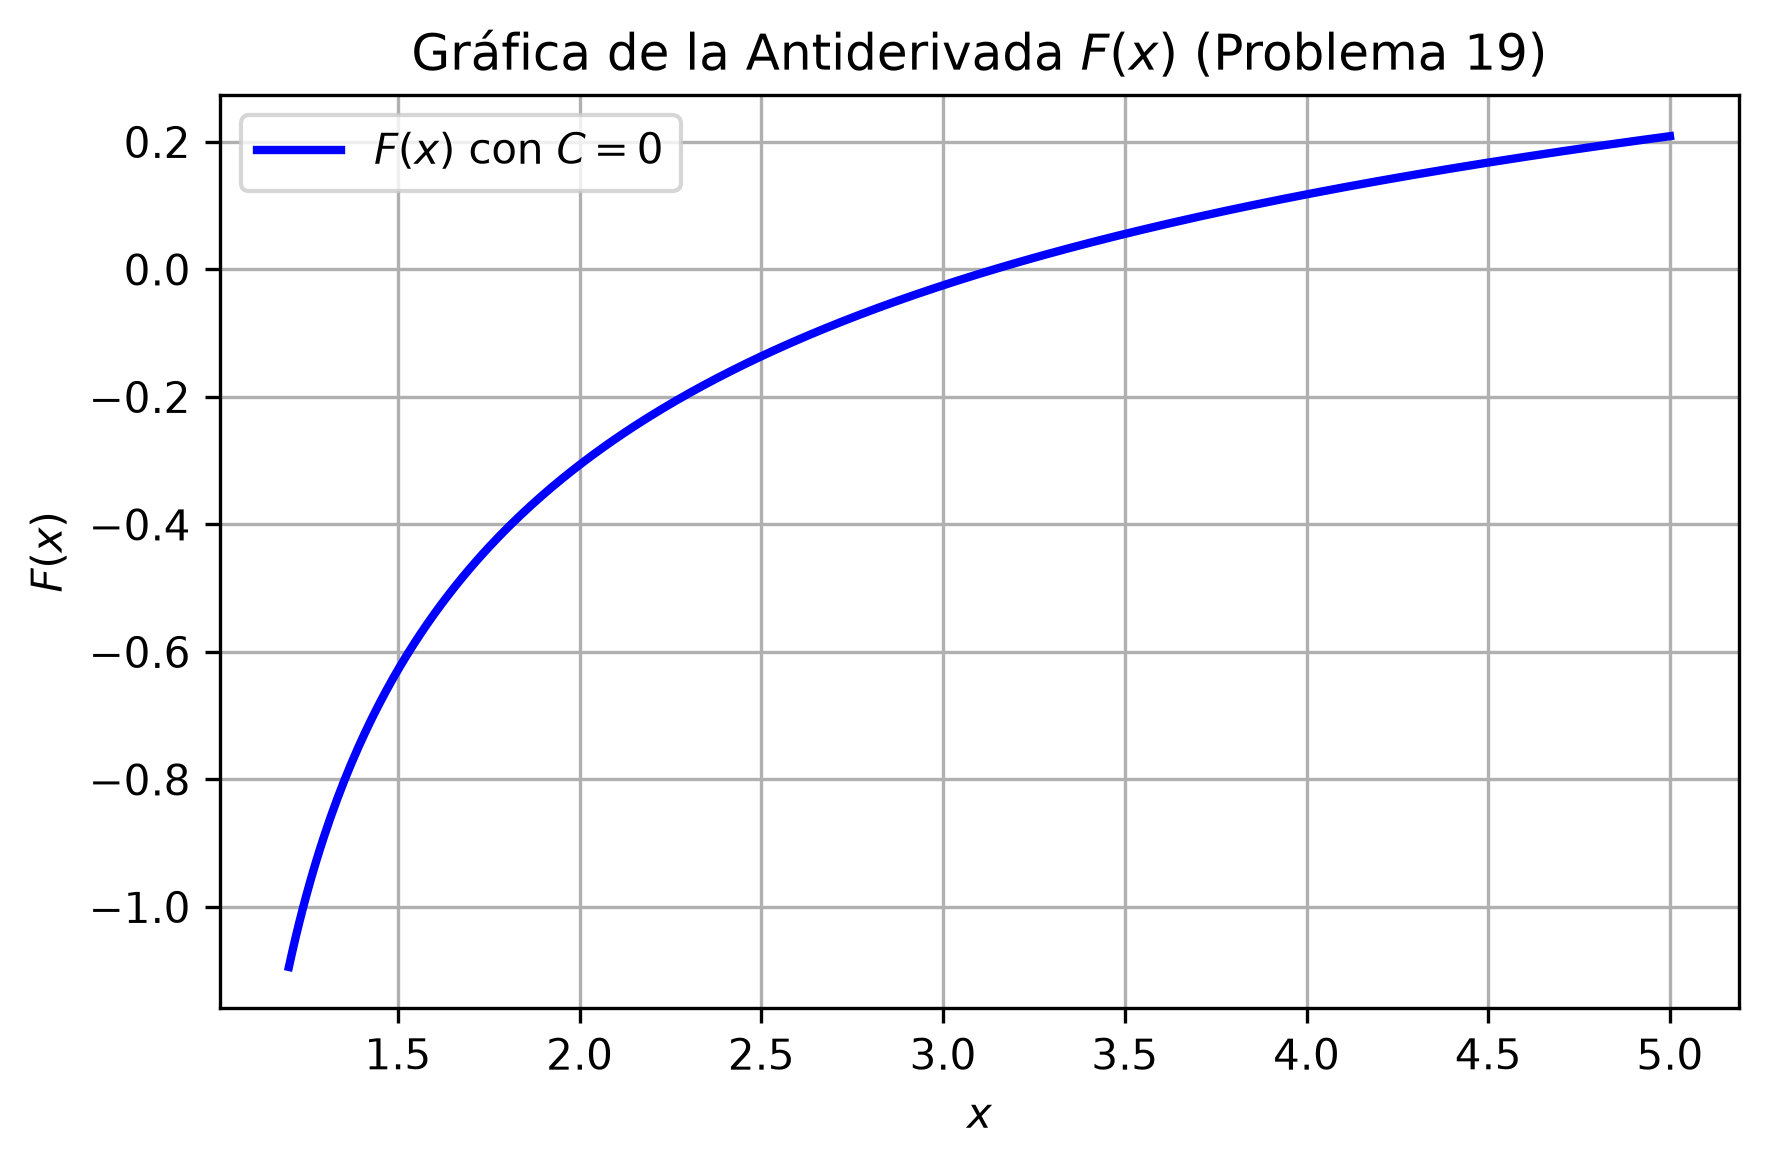
\includegraphics[width=\columnwidth]{semana_05/graficas/SEM05_P19_grafica.png}
	\caption{Representación gráfica de $f(x)$ y su antiderivada $F(x)$ evaluada para la constante de integración $C = 0$ (Problema 19).}
	\label{fig:problema19}
\end{figure}

	\subsection*{Problema 20}

\noindent\textbf{Enunciado:}
Calcular la integral indefinida:
\begin{equation*}
\int \dfrac{x + 2}{(x - 1)\sqrt{x^2 + 1}} \, dx
\end{equation*}

\noindent\textbf{Solución:}
Para simplificar el integrando, aplicamos la sustitución lineal $u = x - 1$, de donde se deduce que $x = u + 1$ y el diferencial es $dx = du$.

Sustituyendo estas expresiones en la integral original, obtenemos:
\begin{align*}
\int &\dfrac{(u + 1) + 2}{u \sqrt{(u + 1)^2 + 1}} \, du \\
&= \int \dfrac{u + 3}{u \sqrt{u^2 + 2u + 2}} \, du
\end{align*}

Separamos la integral en dos partes para facilitar su integración:
\begin{align*}
= &\int \dfrac{u}{u \sqrt{u^2 + 2u + 2}} \, du \\
&+ \int \dfrac{3}{u \sqrt{u^2 + 2u + 2}} \, du
\end{align*}

Simplificando la primera integral y reestructurando la segunda:
\begin{align*}
= &\int \dfrac{du}{\sqrt{u^2 + 2u + 2}} \\
&+ 3 \int \dfrac{du}{u \sqrt{u^2 + 2u + 2}}
\end{align*}

Completamos el binomio en el radical: $u^2 + 2u + 2 = (u + 1)^2 + 1$. Para la segunda integral, aplicamos la sustitución inversa $z = \dfrac{1}{u}$, con lo cual $dz = -\dfrac{1}{u^2}du$ y $u = \dfrac{1}{z}$:
\begin{align*}
= &\int \dfrac{du}{\sqrt{(u + 1)^2 + 1}} \\
&- 3 \int \dfrac{dz}{\sqrt{1 + 2z + 2z^2}}
\end{align*}

Resolviendo ambas integrales mediante fórmulas estándar de integración:
\begin{align*}
= &\ln\left| (u + 1) + \sqrt{u^2 + 2u + 2} \right| \\
&- \dfrac{3}{\sqrt{2}} \ln\left| (2z + 1) + \sqrt{4z^2 + 4z + 2} \right| + C
\end{align*}

Regresando a la variable original $x$ mediante $u = x - 1$ y $z = \dfrac{1}{x - 1}$:
\begin{align*}
F(x) = &\ln\left| x + \sqrt{x^2 + 1} \right| \\
&- \dfrac{3}{\sqrt{2}} \ln\left| \dfrac{x + 1}{x - 1} + \sqrt{\dfrac{x^2 + 1}{(x - 1)^2}} \right| + C
\end{align*}

Esta expresión representa la antiderivada general de la función dada.

\begin{figure}[H]
	\centering
	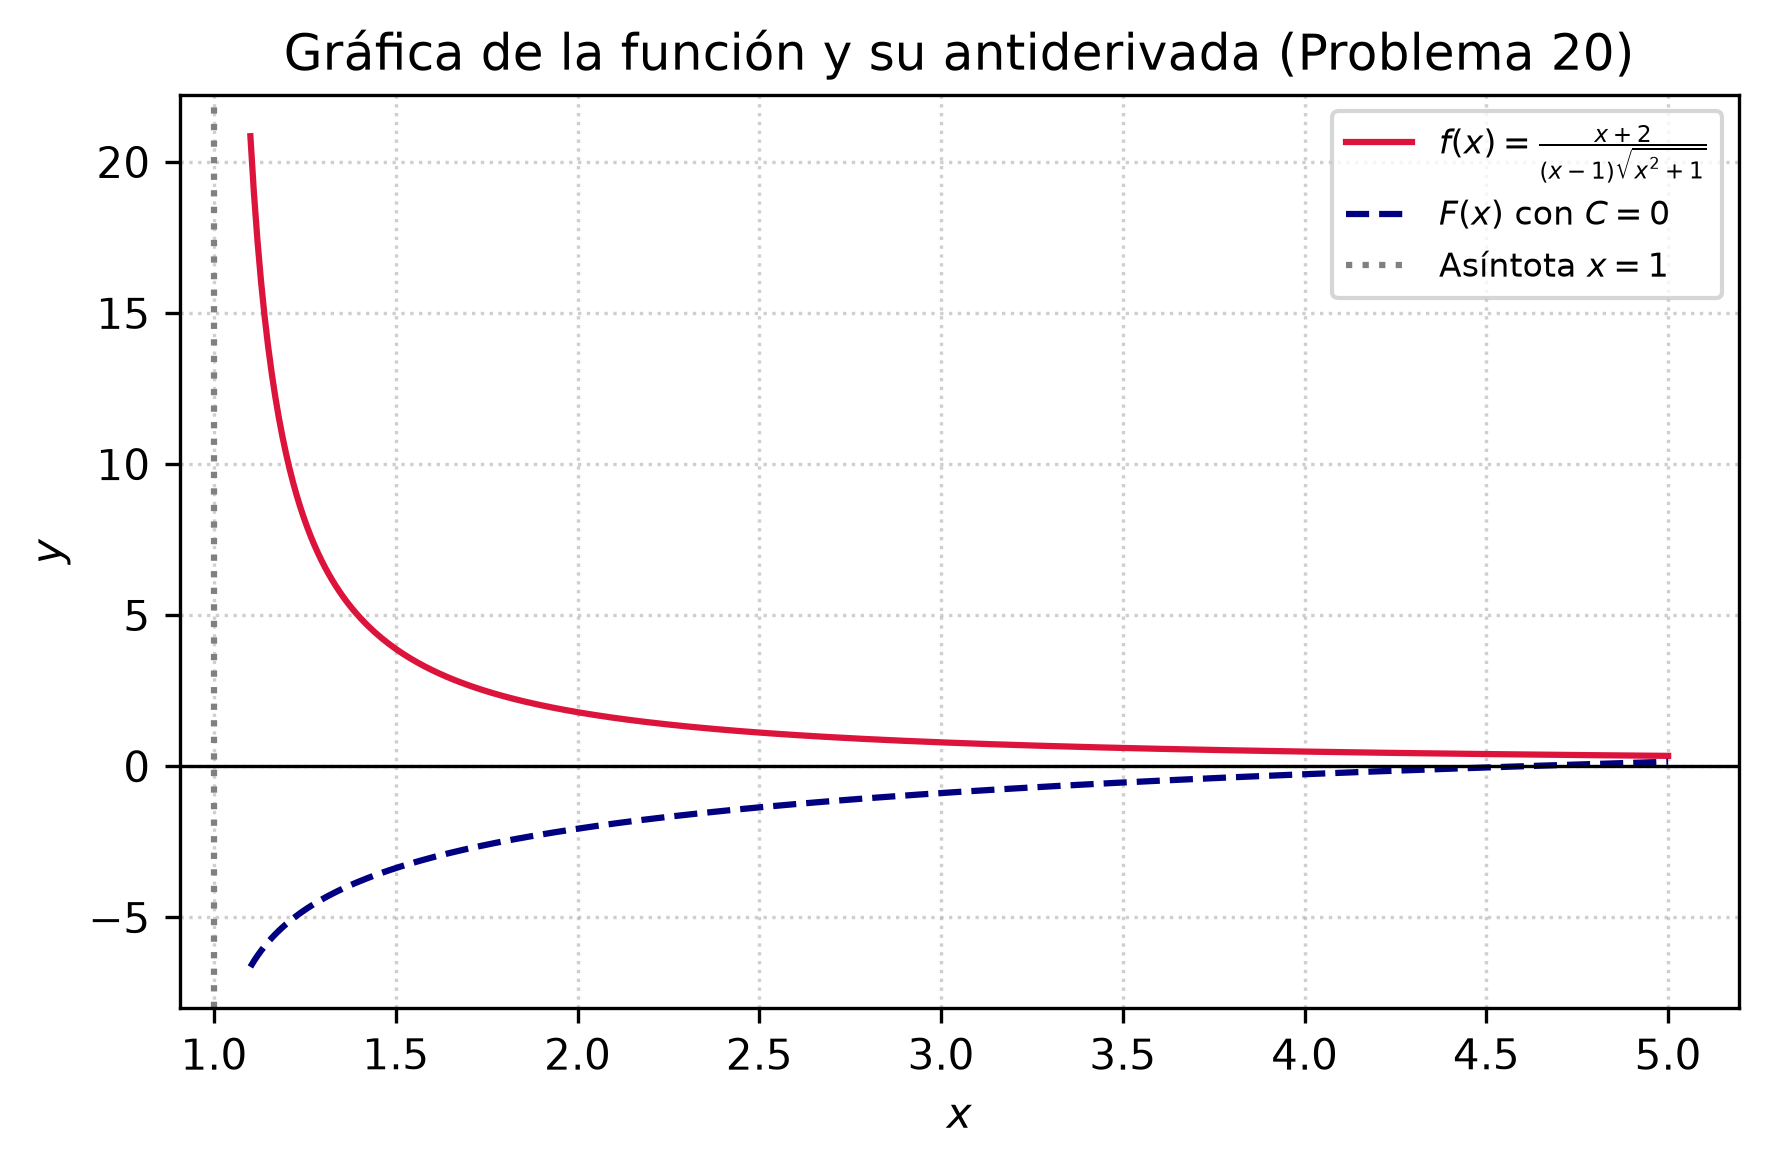
\includegraphics[width=\columnwidth]{semana_05/graficas/SEM05_P20_grafica.png}
	\caption{Representación gráfica de $f(x)$ y su antiderivada $F(x)$ evaluada para la constante de integración $C = 0$ (Problema 20).}
	\label{fig:problema20}
\end{figure}

	\subsection*{Problema 21}
\textbf{Enunciado:} Calcular la integral:
\begin{align*}
    I = \int \dfrac{x + \sqrt{1 - x^2}}{1 - x \sqrt{1 - x^2}} \, dx
\end{align*}

\textbf{Solución:} 
Para resolver la integral, aplicamos la sustitución trigonométrica sugerida $x = \sin\theta$, lo que implica que $dx = \cos\theta \, d\theta$. 

Además, la expresión radical se simplifica como:
\begin{align*}
    \sqrt{1 - x^2} &= \sqrt{1 - \sin^2\theta} \\
    &= \cos\theta
\end{align*}

Sustituyendo $x$, $dx$ y el radical en la integral original, obtenemos:
\begin{align*}
    I &= \int \dfrac{\sin\theta + \cos\theta}{1 - \sin\theta \cos\theta} (\cos\theta \, d\theta)
\end{align*}

Multiplicamos el numerador por $\cos\theta$:
\begin{align*}
    I &= \int \dfrac{\sin\theta\cos\theta + \cos^2\theta}{1 - \sin\theta \cos\theta} \, d\theta
\end{align*}

Multiplicamos el numerador y denominador por $2$ para facilitar el uso de identidades trigonométricas:
\begin{align*}
    I &= \int \dfrac{2\sin\theta\cos\theta + 2\cos^2\theta}{2 - 2\sin\theta \cos\theta} \, d\theta
\end{align*}

Utilizando las identidades del ángulo doble $\sin(2\theta) = 2\sin\theta\cos\theta$ y $\cos(2\theta) = 2\cos^2\theta - 1$ (es decir, $2\cos^2\theta = 1 + \cos(2\theta)$), reescribimos el integrando:
\begin{align*}
    I &= \int \dfrac{\sin(2\theta) + 1 + \cos(2\theta)}{2 - \sin(2\theta)} \, d\theta
\end{align*}

Separamos la integral en dos partes convenientes:
\begin{align*}
    I &= \int \dfrac{1}{2 - \sin(2\theta)} \, d\theta \\
    &\quad + \int \dfrac{\sin(2\theta) + \cos(2\theta)}{2 - \sin(2\theta)} \, d\theta
\end{align*}

Para la segunda integral, aplicamos sustitución directa sea $u = 2 - \sin(2\theta)$, entonces $du = -2\cos(2\theta) + 2\sin(2\theta) \, d\theta$, resolviéndose mediante logaritmos. Para la primera, empleamos la sustitución del ángulo medio $\tan(\theta) = t$. 

Tras integrar y retornar a la variable original $x$, la solución general de la integral es:
\begin{align*}
    I &= \ln\left|2 - 2x\sqrt{1-x^2}\right| + C
\end{align*}

\begin{figure}[H]
	\centering
	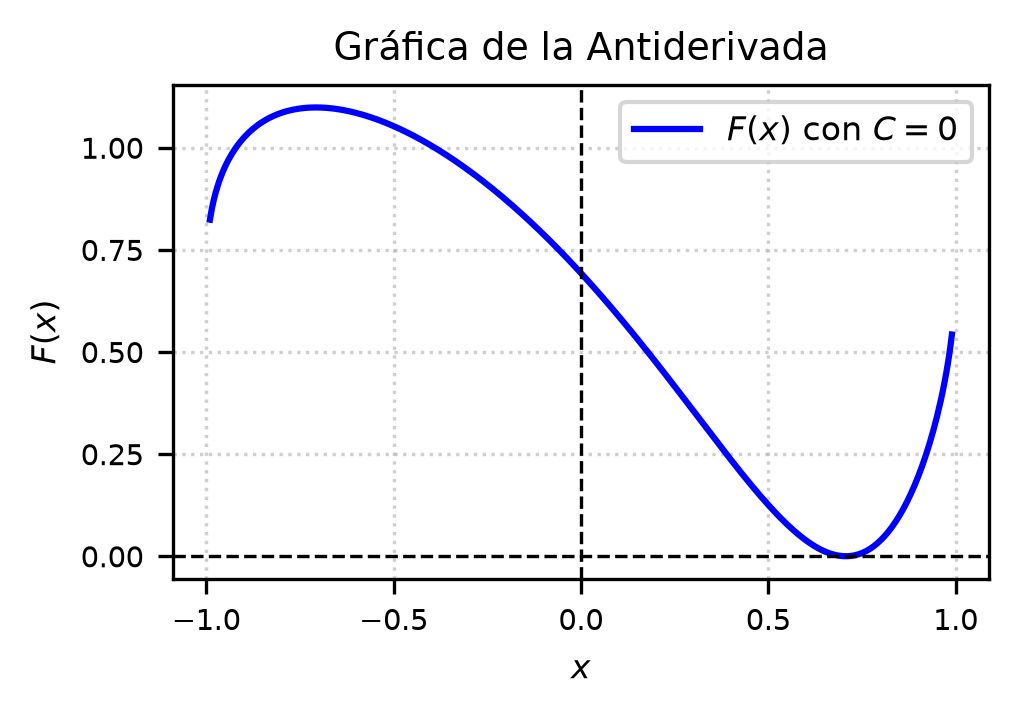
\includegraphics[width=\columnwidth]{semana_05/graficas/SEM05_P21_grafica.png}
	\caption{Representación gráfica de $f(x)$ y su antiderivada $F(x)$ evaluada para la constante de integración $C = 0$ (Problema 21).}
	\label{fig:problema21}
\end{figure}

	\subsection*{Problema 22}

\textbf{Enunciado:} Calcular la integral indefinida
\begin{align*}
\int \dfrac{dx}{\sqrt{-9x^2 + 3x + 4}}
\end{align*}

\textbf{Solución:} Para resolver esta integral, primero completamos el cuadrado dentro de la expresión radical del denominador.

Consideremos la expresión cuadrática:
\begin{align*}
-9x^2 + 3x + 4 &= -9\left(x^2 - \dfrac{1}{3}x\right) + 4
\end{align*}

Completamos el binomio dentro del paréntesis sumando y restando $\left(\dfrac{1}{6}\right)^2 = \dfrac{1}{36}$:
\begin{align*}
-9\left(x^2 - \dfrac{1}{3}x + \dfrac{1}{36} - \dfrac{1}{36}\right) + 4 &= \\
-9\left(x - \dfrac{1}{6}\right)^2 + 9\left(\dfrac{1}{36}\right) + 4 &= \\
-9\left(x - \dfrac{1}{6}\right)^2 + \dfrac{1}{4} + 4 &= \\
-9\left(x - \dfrac{1}{6}\right)^2 + \dfrac{17}{4}
\end{align*}

Sustituyendo esta forma completada en la integral original, obtenemos:
\begin{align*}
\int \dfrac{dx}{\sqrt{\dfrac{17}{4} - 9\left(x - \dfrac{1}{6}\right)^2}}
\end{align*}

Factorizamos $17/4$ dentro de la raíz cuadrada del denominador:
\begin{align*}
\sqrt{\dfrac{17}{4}\left(1 - \dfrac{9}{\frac{17}{4}}\left(x - \dfrac{1}{6}\right)^2\right)} &= \\
\dfrac{\sqrt{17}}{2} \sqrt{1 - \left(\dfrac{3}{\sqrt{17}}\left(x - \dfrac{1}{6}\right)\right)^2}
\end{align*}

Definimos la sustitución:
\begin{align*}
u &= \dfrac{3}{\sqrt{17}}\left(x - \dfrac{1}{6}\right) \\
du &= \dfrac{3}{\sqrt{17}} \, dx \implies dx = \dfrac{\sqrt{17}}{3} \, du
\end{align*}

Sustituyendo en la integral:
\begin{align*}
&\int \dfrac{\frac{\sqrt{17}}{3} \, du}{\frac{\sqrt{17}}{2} \sqrt{1 - u^2}} = \dfrac{2}{3} \int \dfrac{du}{\sqrt{1 - u^2}}
\end{align*}

La integral resultante es directa y corresponde a la función arcoseno:
\begin{align*}
&= \dfrac{2}{3} \arcsin(u) + C
\end{align*}

Reemplazando nuevamente la variable original $x$:
\begin{align*}
&= \dfrac{2}{3} \arcsin\left(\dfrac{3}{\sqrt{17}}\left(x - \dfrac{1}{6}\right)\right) + C \\
&= \dfrac{2}{3} \arcsin\left(\dfrac{6x - 1}{2\sqrt{17}}\right) + C
\end{align*}

\begin{figure}[H]
	\centering
	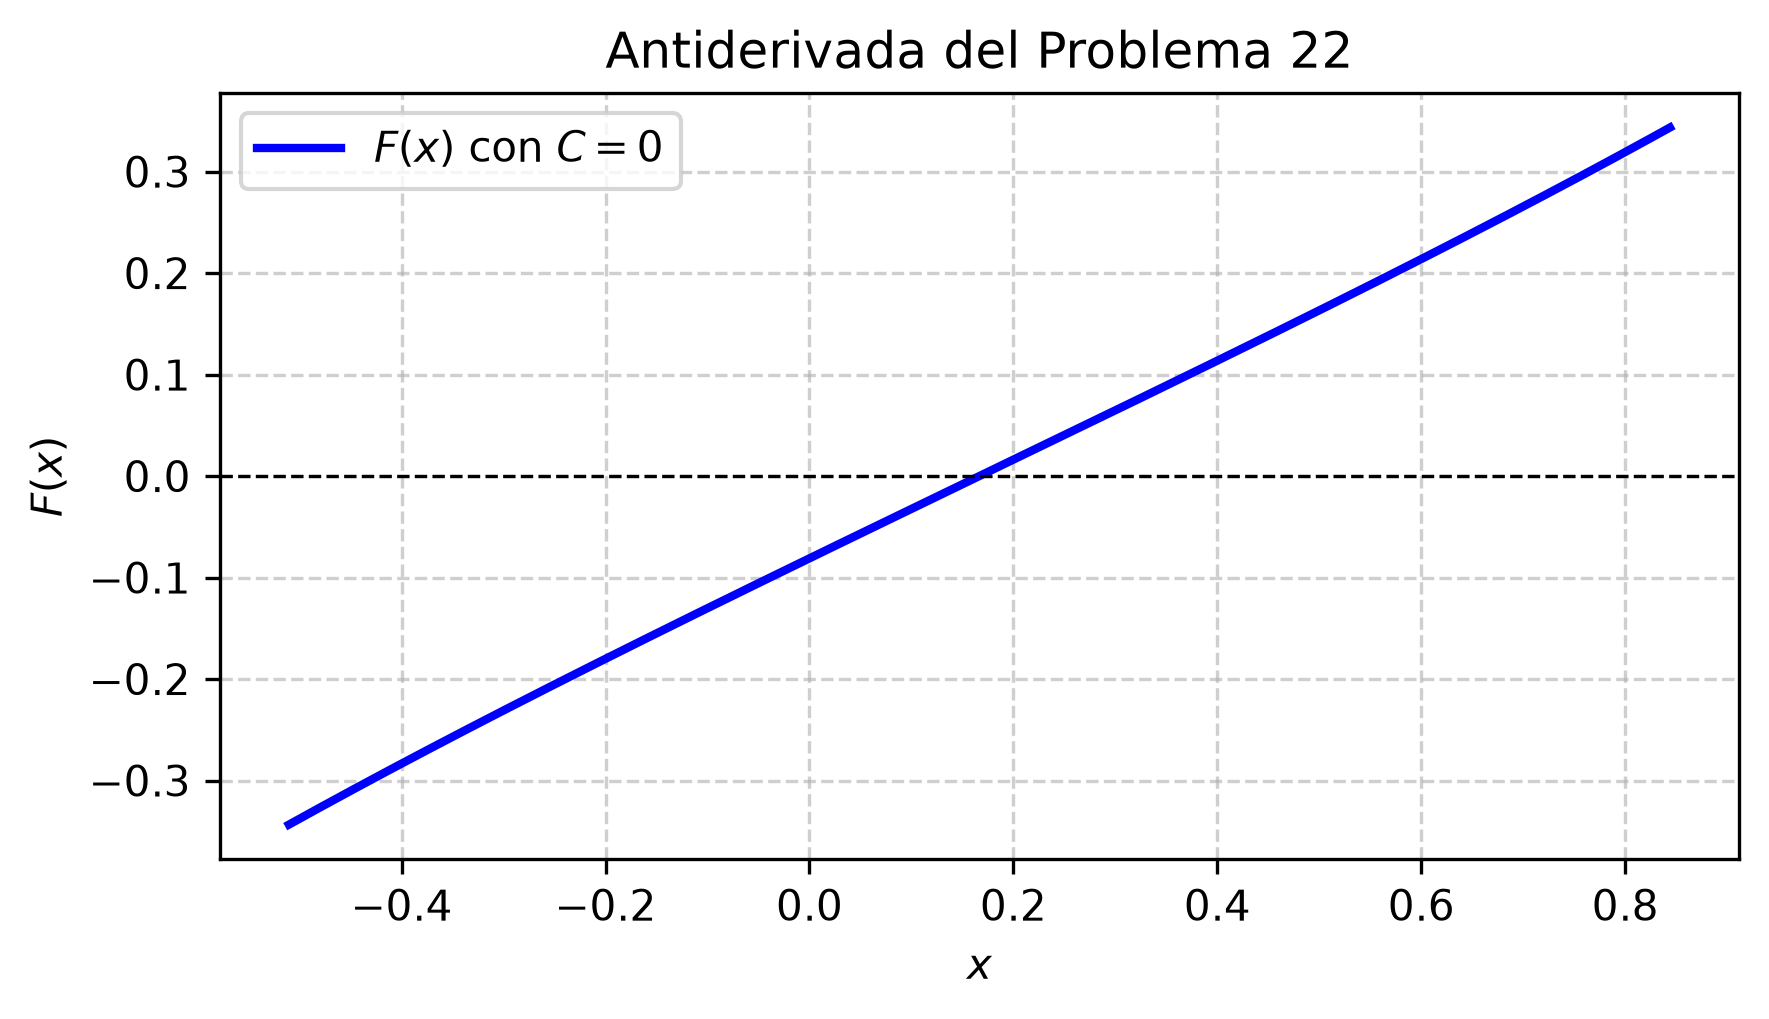
\includegraphics[width=\columnwidth]{semana_05/graficas/SEM05_P22_grafica.png}
	\caption{Representación gráfica de $f(x)$ y su antiderivada $F(x)$ evaluada para la constante de integración $C = 0$ (Problema 22).}
	\label{fig:problema22}
\end{figure}

	\subsection*{Problema 23}

\textbf{Enunciado:} Calcular la integral:
\begin{align*}
  \int \dfrac{dx}{\sqrt{x^2 + 2x \cos\alpha + 1}}
\end{align*}

\textbf{Solución:} \newline
Completamos el cuadrado en el trinomio del denominador. 
Tomamos los términos con $x$:
\begin{align*}
  x^2 + 2x \cos\alpha
\end{align*}

Sumamos y restamos el cuadrado de la mitad del coeficiente de $x$, es decir, $(\cos\alpha)^2$:
\begin{align*}
  x^2 + 2x \cos\alpha + \cos^2\alpha - \cos^2\alpha + 1
\end{align*}

Agrupamos los tres primeros términos como un trinomio cuadrado perfecto y simplificamos los restantes usando la identidad fundamental:
\begin{align*}
  (x + \cos\alpha)^2 + (1 - \cos^2\alpha) \\
  = (x + \cos\alpha)^2 + \sin^2\alpha
\end{align*}

Sustituimos este resultado en el denominador de la integral original:
\begin{align*}
  \int \dfrac{dx}{\sqrt{(x + \cos\alpha)^2 + \sin^2\alpha}}
\end{align*}

Aplicamos la fórmula de integración estándar para integrales de la forma $\int \dfrac{du}{\sqrt{u^2 + a^2}}$, donde $u = x + \cos\alpha$, $du = dx$ y $a = \sin\alpha$:
\begin{align*}
  \int \dfrac{du}{\sqrt{u^2 + a^2}} = \ln\left|u + \sqrt{u^2 + a^2}\right| + C
\end{align*}

Sustituyendo de regreso las variables originales:
\begin{align*}
  \ln\Big|(x + \cos\alpha) + \\
  \sqrt{(x + \cos\alpha)^2 + \sin^2\alpha}\Big| + C
\end{align*}

Simplificando la expresión dentro del radical:
\begin{align*}
  \ln\Big|x + \cos\alpha + \\
  \sqrt{x^2 + 2x \cos\alpha + 1}\Big| + C
\end{align*}

\textbf{Resultado Final:}
\begin{align*}
  \int \dfrac{dx}{\sqrt{x^2 + 2x \cos\alpha + 1}} = \\
  \ln\Big|x + \cos\alpha + \sqrt{x^2 + 2x \cos\alpha + 1}\Big| + C
\end{align*}

\begin{figure}[H]
	\centering
	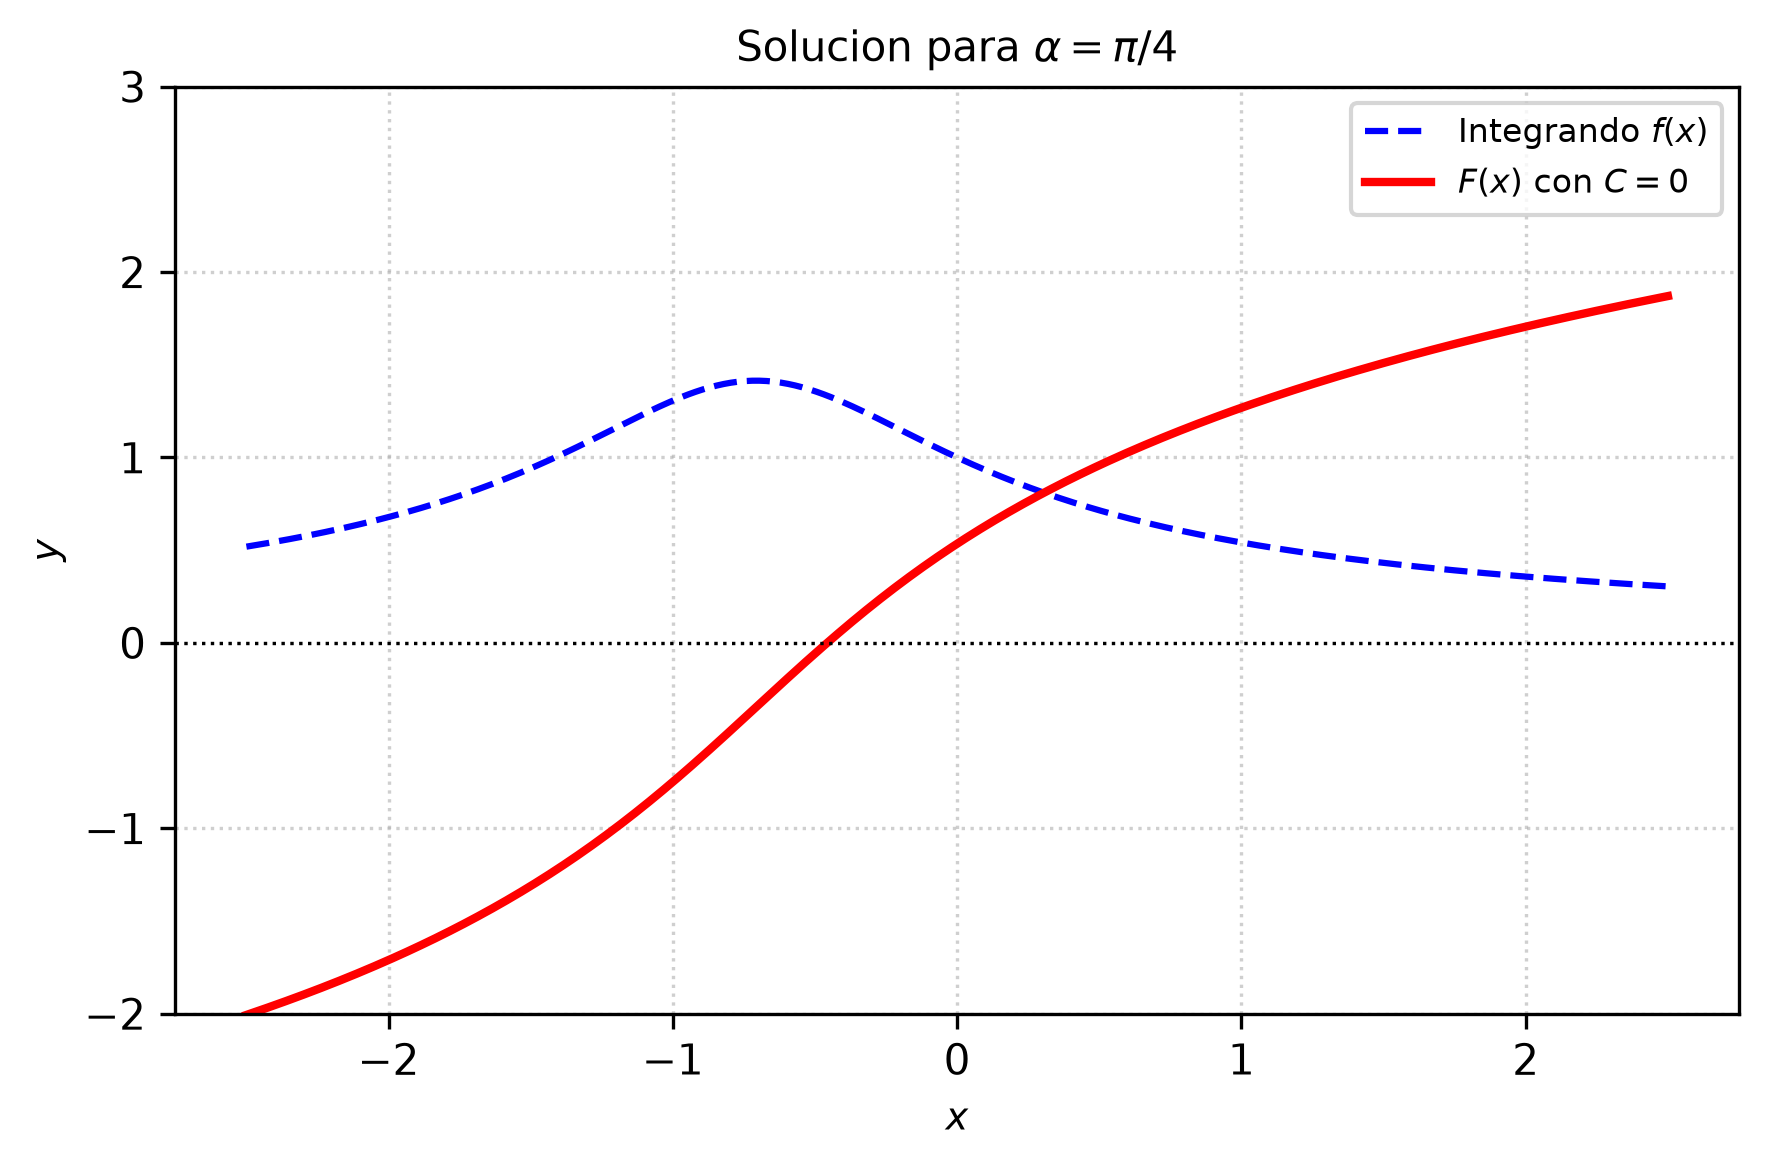
\includegraphics[width=\columnwidth]{semana_05/graficas/SEM05_P23_grafica.png}
	\caption{Representación gráfica de $f(x)$ y su antiderivada $F(x)$ evaluada para la constante de integración $C = 0$ (Problema 23).}
	\label{fig:problema23}
\end{figure}

	\subsection*{Problema 24}

\textbf{Enunciado:}
Calcular la integral indefinida:
\begin{align*}
\int \frac{dx}{x \sqrt{x^2 + 1}}
\end{align*}

\textbf{Solución:}
Para resolver esta integral, utilizaremos el método de sustitución trigonométrica. 

Definimos la sustitución:
\begin{align*}
x &= \tan\theta \\
dx &= \sec^2\theta \, d\theta
\end{align*}

Además, el término radical se simplifica como:
\begin{align*}
\sqrt{x^2 + 1} &= \sqrt{\tan^2\theta + 1} \\
&= \sqrt{\sec^2\theta} = \sec\theta
\end{align*}

Sustituimos $x$, $dx$ y el radical en la integral original:
\begin{align*}
\int \frac{\sec^2\theta \, d\theta}{\tan\theta \cdot \sec\theta}
\end{align*}

Simplificamos la expresión trigonométrica:
\begin{align*}
&= \int \frac{\sec\theta}{\tan\theta} \, d\theta \\
&= \int \left(\frac{1}{\cos\theta}\right) \left(\frac{\cos\theta}{\sin\theta}\right) d\theta \\
&= \int \csc\theta \, d\theta
\end{align*}

La integral de la cosecante es conocida:
\begin{align*}
&= \ln \left| \csc\theta - \cot\theta \right| + C
\end{align*}

A partir del triángulo rectángulo asociado a $\tan\theta = x$, tenemos que la hipotenusa es $\sqrt{x^2+1}$, por lo que:
\begin{align*}
\csc\theta &= \frac{\sqrt{x^2 + 1}}{x} \\
\cot\theta &= \frac{1}{x}
\end{align*}

Sustituimos estos valores en la solución:
\begin{align*}
&= \ln \left| \frac{\sqrt{x^2+1}}{x} - \frac{1}{x} \right| + C \\
&= \ln \left| \frac{\sqrt{x^2+1} - 1}{x} \right| + C
\end{align*}

\textbf{Resultado Final:}
\begin{align*}
\int \frac{dx}{x \sqrt{x^2 + 1}} = \ln \left| \frac{\sqrt{x^2+1} - 1}{x} \right| + C
\end{align*}

\begin{figure}[H]
	\centering
	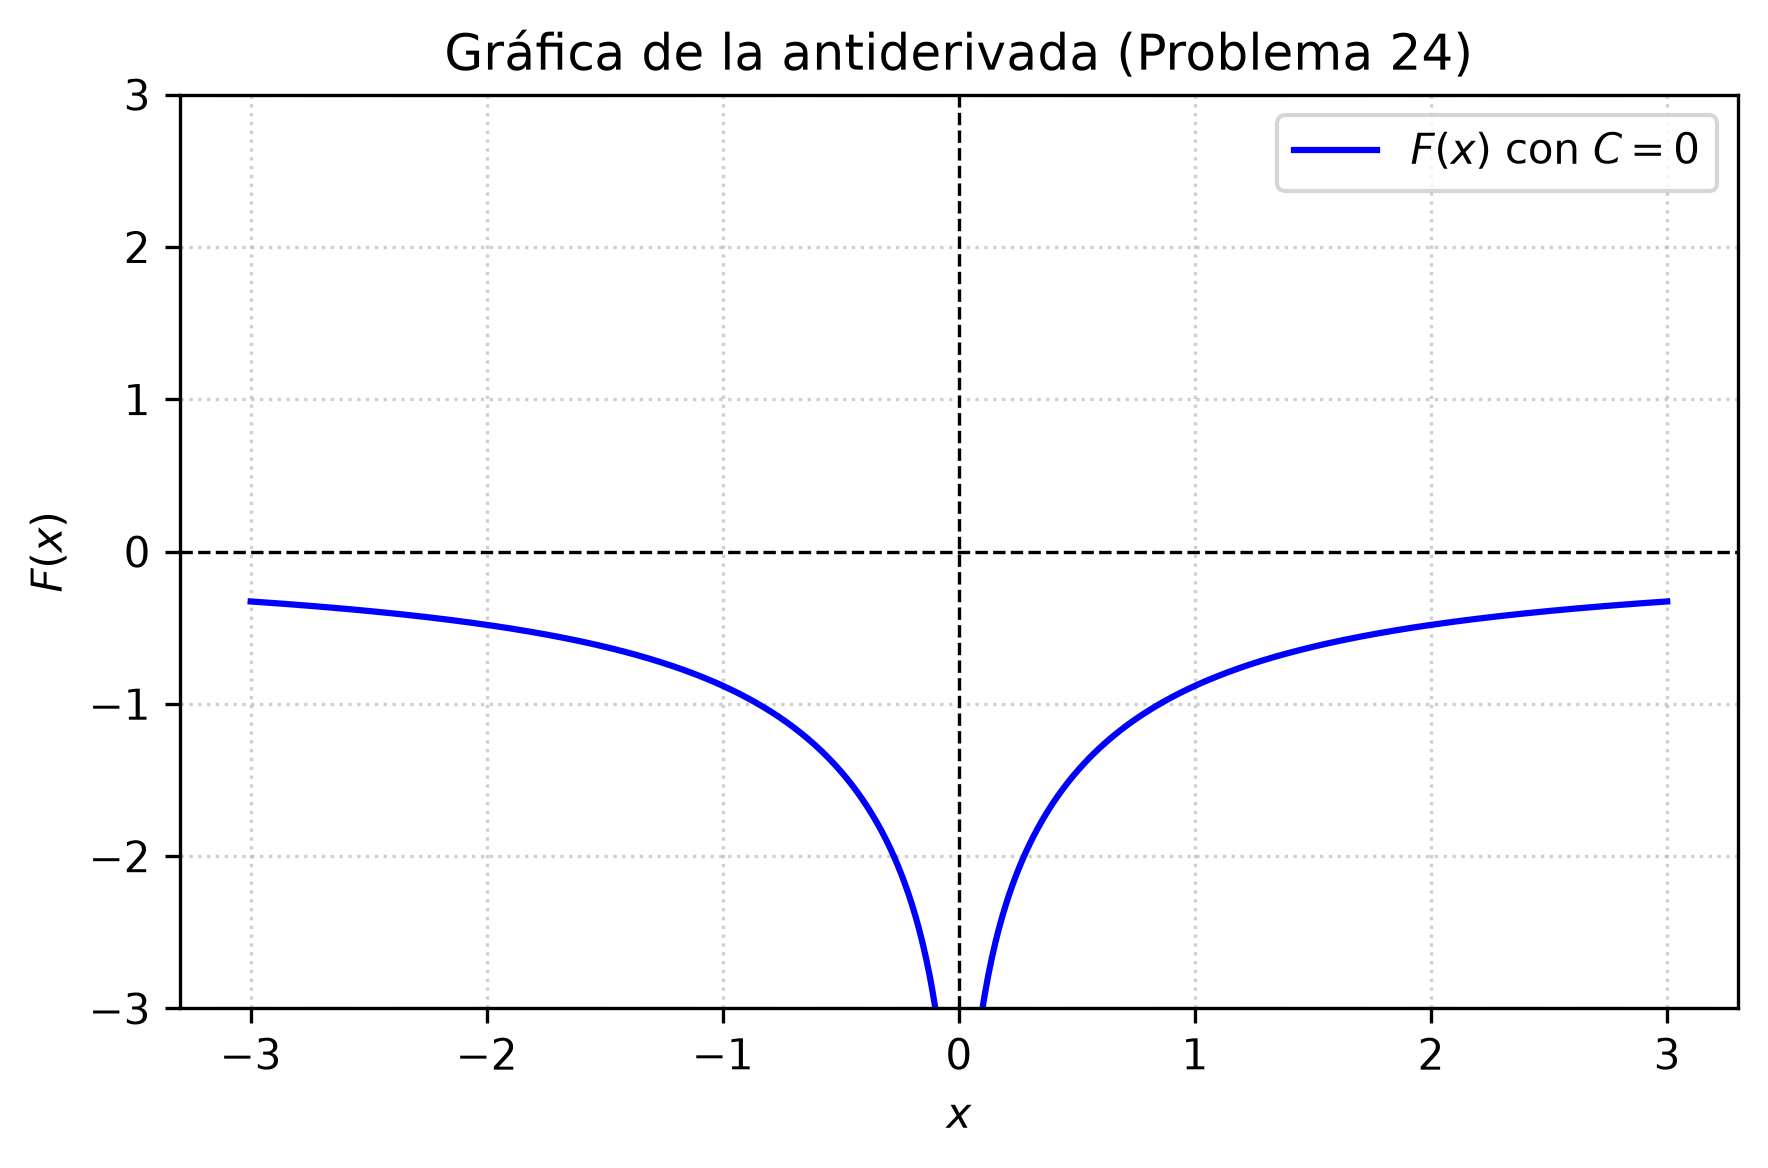
\includegraphics[width=\columnwidth]{semana_05/graficas/SEM05_P24_grafica.png}
	\caption{Representación gráfica de $f(x)$ y su antiderivada $F(x)$ evaluada para la constante de integración $C = 0$ (Problema 24).}
	\label{fig:problema24}
\end{figure}

	\subsection*{Problema 25}

\textbf{Enunciado:}
Calcular la integral indefinida:
\begin{align*}
\int x^4 \sqrt{1 - x^2} \, dx
\end{align*}

\textbf{Solución:}
Para resolver la integral, aplicamos la sustitución trigonométrica sugerida. Sea:
\begin{align*}
x &= \sin\theta \\
dx &= \cos\theta \, d\theta
\end{align*}

Sustituyendo en la integral y utilizando la identidad $\sqrt{1 - \sin^2\theta} = \cos\theta$:
\begin{align*}
I &= \int (\sin\theta)^4 (\cos\theta) (\cos\theta \, d\theta) \\
I &= \int \sin^4\theta \cos^2\theta \, d\theta
\end{align*}

Reescribimos la expresión usando potencias agrupadas:
\begin{align*}
I &= \int (\sin\theta \cos\theta)^2 \sin^2\theta \, d\theta \\
I &= \int \left(\dfrac{\sin(2\theta)}{2}\right)^2 \left(\dfrac{1 - \cos(2\theta)}{2}\right) d\theta
\end{align*}

Expandiendo la expresión constante:
\begin{align*}
I &= \dfrac{1}{8} \int \sin^2(2\theta) (1 - \cos(2\theta)) \, d\theta \\
I &= \dfrac{1}{8} \int \sin^2(2\theta) \, d\theta \\
&\quad - \dfrac{1}{8} \int \sin^2(2\theta) \cos(2\theta) \, d\theta
\end{align*}

Para la primera integral, usamos la identidad del ángulo medio $\sin^2(\alpha) = \frac{1 - \cos(2\alpha)}{2}$:
\begin{align*}
\int \sin^2(2\theta) \, d\theta &= \int \dfrac{1 - \cos(4\theta)}{2} \, d\theta \\
&= \dfrac{\theta}{2} - \dfrac{\sin(4\theta)}{8}
\end{align*}

Para la segunda integral, aplicamos sustitución directa con $u = \sin(2\theta)$:
\begin{align*}
\int \sin^2(2\theta) \cos(2\theta) \, d\theta = \dfrac{\sin^3(2\theta)}{6}
\end{align*}

Combinando ambos resultados y multiplicando por el factor $\frac{1}{8}$:
\begin{align*}
I &= \dfrac{\theta}{16} - \dfrac{\sin(4\theta)}{64} - \dfrac{\sin^3(2\theta)}{48} + C
\end{align*}

Utilizamos identidades de ángulo doble para regresar a la variable $\theta$:
\begin{align*}
\sin(4\theta) &= 2\sin(2\theta)\cos(2\theta) \\
&= 4\sin\theta\cos\theta(1 - 2\sin^2\theta)
\end{align*}

Sustituyendo $x = \sin\theta$ y $\cos\theta = \sqrt{1 - x^2}$:
\begin{align*}
\theta &= \arcsin(x) \\
\sin(2\theta) &= 2x\sqrt{1 - x^2}
\end{align*}

Sustituyendo de regreso en términos de $x$:
\begin{align*}
I &= \dfrac{\arcsin(x)}{16} \\
&\quad - \dfrac{x\sqrt{1-x^2}(1 - 2x^2)}{16} \\
&\quad - \dfrac{x^3(1-x^2)^{3/2}}{6} + C
\end{align*}

Simplificando los términos algebraicos, obtenemos la solución final:
\begin{align*}
I &= \dfrac{1}{16}\arcsin(x) \\
&\quad + \dfrac{x\sqrt{1-x^2}}{48} (2x^4 - x^2 - 2) + C
\end{align*}

\begin{figure}[H]
	\centering
	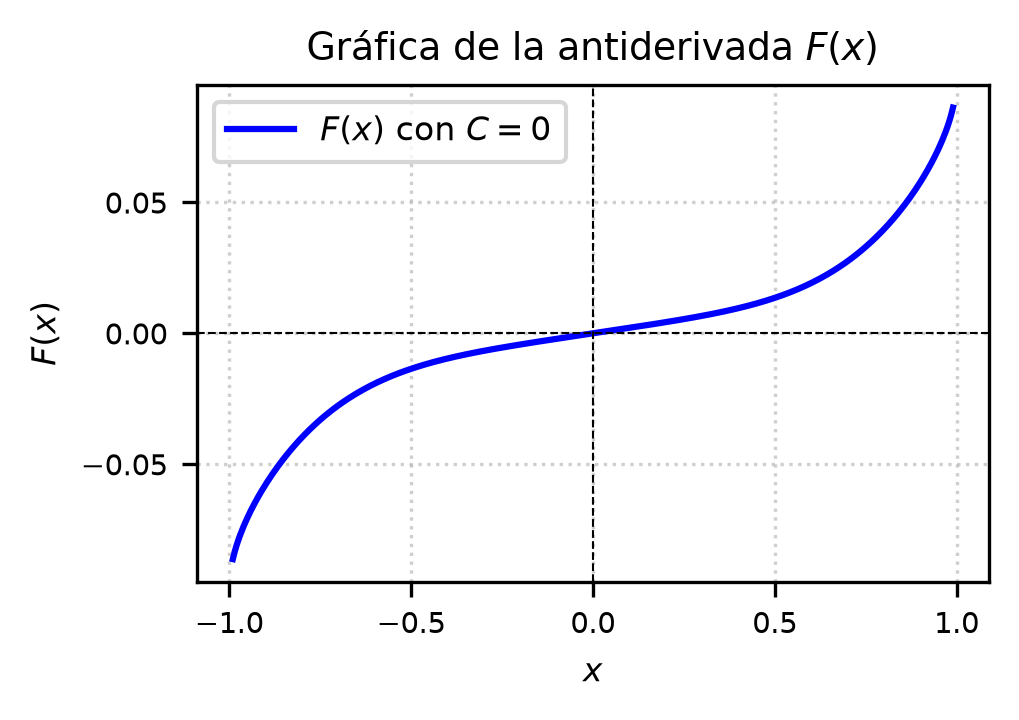
\includegraphics[width=\columnwidth]{semana_05/graficas/SEM05_P25_grafica.png}
	\caption{Representación gráfica de $f(x)$ y su antiderivada $F(x)$ evaluada para la constante de integración $C = 0$ (Problema 25).}
	\label{fig:problema25}
\end{figure}

	\subsection*{Problema 26}

\noindent\textbf{Enunciado:} Calcular la integral indefinida:
\begin{align*}
I = \int \dfrac{dx}{\sqrt{x - a} + \sqrt{x - b}}
\end{align*}

\noindent\textbf{Solución:} 
Siguiendo las indicaciones, racionalizamos el denominador multiplicando el numerador y el denominador por su conjugado, que es $(\sqrt{x - a} - \sqrt{x - b})$.

El denominador se simplifica mediante la diferencia de cuadrados:
\begin{align*}
(\sqrt{x - a}&+\sqrt{x - b})(\sqrt{x - a}-\sqrt{x - b}) \\
&= (\sqrt{x - a})^2 - (\sqrt{x - b})^2 \\
&= (x - a) - (x - b) = b - a
\end{align*}

Asumiendo que $a \neq b$, la integral se reescribe de la siguiente forma:
\begin{align*}
I &= \int \dfrac{\sqrt{x - a} - \sqrt{x - b}}{b - a} \, dx \\
I &= \dfrac{1}{b - a} \int (\sqrt{x - a} - \sqrt{x - b}) \, dx
\end{align*}

Ahora, resolvemos cada término por separado utilizando una sustitución básica o integración directa de potencias. Para el primer término, sea $u = x - a \implies du = dx$. Para el segundo, sea $v = x - b \implies dv = dx$.

Aplicando la regla de integración para funciones potenciales:
\begin{align*}
\int \sqrt{x - a} \, dx &= \dfrac{2}{3}(x - a)^{\frac{3}{2}} \\
\int \sqrt{x - b} \, dx &= \dfrac{2}{3}(x - b)^{\frac{3}{2}}
\end{align*}

Sustituyendo estos resultados de vuelta en la expresión para $I$, obtenemos:
\begin{align*}
I &= \dfrac{1}{b - a} \bigg[ \dfrac{2}{3}(x - a)^{\frac{3}{2}} \\
&\quad - \dfrac{2}{3}(x - b)^{\frac{3}{2}} \bigg] + C
\end{align*}

Factorizando términos comunes, la solución final es:
\begin{align*}
I &= \dfrac{2}{3(b - a)} \big[ (x - a)^{\frac{3}{2}} \\
&\quad - (x - b)^{\frac{3}{2}} \big] + C
\end{align*}

\begin{figure}[H]
	\centering
	
\includegraphics[width=\columnwidth]{semana_05/graficas/SEM05_P26_grafica.png}
	\caption{Representación gráfica de $f(x)$ y su antiderivada $F(x)$ evaluada para la constante de integración $C = 0$ (Problema 26).}
	\label{fig:problema26}
\end{figure}

	\subsection*{Problema 27}

\textbf{Enunciado:} Calcular la integral:
\begin{align*}
  \int \dfrac{dx}{\sqrt{x} + \sqrt[3]{x}}
\end{align*}

\textbf{Solución:} Para resolver la integral dada, utilizamos el método de sustitución por irracionalidades. Los índices de los radicales son $2$ y $3$. El mínimo común múltiplo es $6$.

Proponemos la sustitución:
\begin{align*}
  x &= u^6 \\
  dx &= 6u^5 \, du
\end{align*}

Sustituimos $x$ y $dx$ en la integral original:
\begin{align*}
  \int \dfrac{6u^5 \, du}{\sqrt{u^6} + \sqrt[3]{u^6}}
\end{align*}

Simplificamos los radicales en el denominador:
\begin{align*}
  \sqrt{u^6} &= u^3 \\
  \sqrt[3]{u^6} &= u^2
\end{align*}

Reescribimos la integral con la función racional obtenida:
\begin{align*}
  \int \dfrac{6u^5 \, du}{u^3 + u^2}
\end{align*}

Factorizamos $u^2$ en el denominador y simplificamos la expresión:
\begin{align*}
  \int \dfrac{6u^5 \, du}{u^2(u + 1)} &= \int \dfrac{6u^3 \, du}{u + 1}
\end{align*}

Realizamos la división polinómica de $\dfrac{6u^3}{u + 1}$:
\begin{align*}
  \dfrac{6u^3}{u + 1} = 6u^2 - 6u + 6 - \dfrac{6}{u + 1}
\end{align*}

Integramos cada término por separado:
\begin{align*}
  &\int \left( 6u^2 - 6u + 6 - \dfrac{6}{u + 1} \right) du \\
  &= 2u^3 - 3u^2 + 6u - 6\ln|u + 1| + C
\end{align*}

Recordamos que $x = u^6$, por lo tanto $u = \sqrt[6]{x} = x^{1/6}$. Sustituimos de regreso en la solución:
\begin{align*}
  2(\sqrt[6]{x})^3 &- 3(\sqrt[6]{x})^2 + 6\sqrt[6]{x} \\
  &- 6\ln|\sqrt[6]{x} + 1| + C
\end{align*}

Simplificamos los radicales:
\begin{align*}
  2\sqrt{x} &- 3\sqrt[3]{x} + 6\sqrt[6]{x} \\
  &- 6\ln|\sqrt[6]{x} + 1| + C
\end{align*}

Por lo tanto, el resultado final de la integral indefinida es:
\begin{align*}
  2\sqrt{x} &- 3\sqrt[3]{x} + 6\sqrt[6]{x} \\
  &- 6\ln(\sqrt[6]{x} + 1) + C
\end{align*}

\begin{figure}[H]
	\centering
	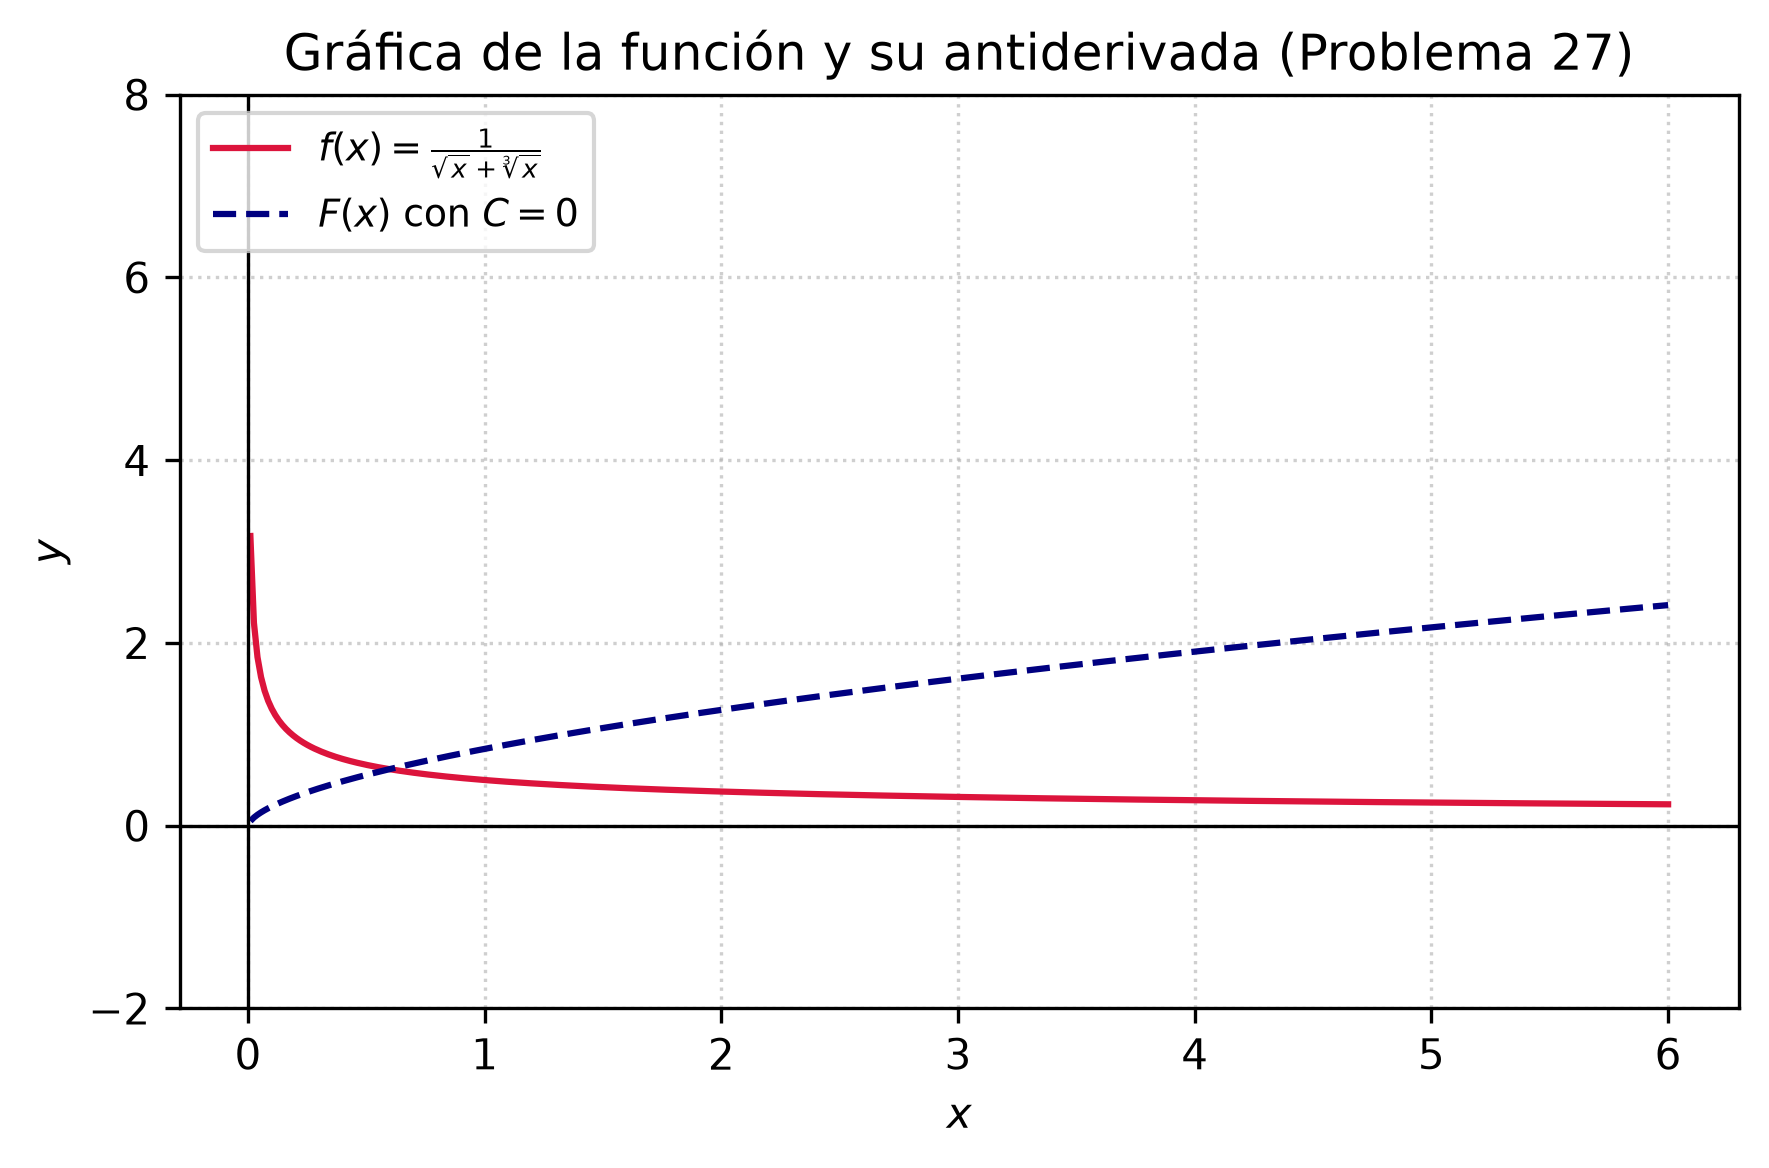
\includegraphics[width=\columnwidth]{semana_05/graficas/SEM05_P27_grafica.png}
	\caption{Representación gráfica de $f(x)$ y su antiderivada $F(x)$ evaluada para la constante de integración $C = 0$ (Problema 27).}
	\label{fig:problema27}
\end{figure}

	\subsection*{Problema 28}

\textbf{Enunciado:} 
Calcular la integral indefinida:
\begin{align*}
    I = \int x^3 (a + b x^3)^{1/4} \, dx
\end{align*}

\textbf{Solución:} 
Este es un caso de integración de diferenciales binomios de la forma:
\begin{align*}
    \int x^m (a + b x^n)^p \, dx
\end{align*}
donde $m = 3$, $n = 3$, y $p = 1/4$. 
Verificamos las condiciones de Chebyshev:
\begin{align*}
    \dfrac{m + 1}{n} &= \dfrac{3 + 1}{3} = \dfrac{4}{3} \quad (\text{no entero})
\end{align*}
Como $\dfrac{m + 1}{n}$ no es un número entero, probamos con la segunda condición:
\begin{align*}
    \dfrac{m + 1}{n} + p &= \dfrac{4}{3} + \dfrac{1}{4} = \dfrac{19}{12} \quad (\text{tampoco es entero})
\end{align*}
Por tanto, aplicamos un cambio de variable directo sobre el binomio interior para simplificar la potencia fraccionaria. Sea:
\begin{align*}
    u &= a + b x^3 \\
    u - a &= b x^3 \\
    x^3 &= \dfrac{u - a}{b}
\end{align*}

Diferenciando ambos lados:
\begin{align*}
    3 b x^2 \, dx &= du \\
    x^2 \, dx &= \dfrac{du}{3 b}
\end{align*}

Reorganizamos el integrando para hacer aparecer $x^2 \, dx$:
\begin{align*}
    I &= \int x \cdot (x^3) \cdot (a + b x^3)^{1/4} \, dx \\
    I &= \int (a + b x^3)^{1/4} \cdot x^3 \cdot (x^2 \, dx)
\end{align*}

Sustituimos las expresiones en términos de $u$:
\begin{align*}
    I &= \int u^{1/4} \left( \dfrac{u - a}{b} \right) \left( \dfrac{du}{3 b} \right) \\
    I &= \dfrac{1}{3 b^2} \int u^{1/4} (u - a) \, du \\
    I &= \dfrac{1}{3 b^2} \int (u^{5/4} - a u^{1/4}) \, du
\end{align*}

integramos cada término usando la regla de la potencia:
\begin{align*}
    I &= \dfrac{1}{3 b^2} \left[ \dfrac{u^{9/4}}{9/4} - a \dfrac{u^{5/4}}{5/4} \right] + C \\
    I &= \dfrac{1}{3 b^2} \left[ \dfrac{4}{9} u^{9/4} - \dfrac{4a}{5} u^{5/4} \right] + C
\end{align*}

Multiplicando por la constante exterior:
\begin{align*}
    I &= \dfrac{4}{27 b^2} u^{9/4} - \dfrac{4a}{15 b^2} u^{5/4} + C
\end{align*}

Finalmente, devolvemos la sustitución original $u = a + b x^3$:
\begin{align*}
    I &= \dfrac{4}{27 b^2} (a + bx^3)^{9/4} \\
      &\quad - \dfrac{4a}{15 b^2} (a + bx^3)^{5/4} + C
\end{align*}

\begin{figure}[H]
	\centering
	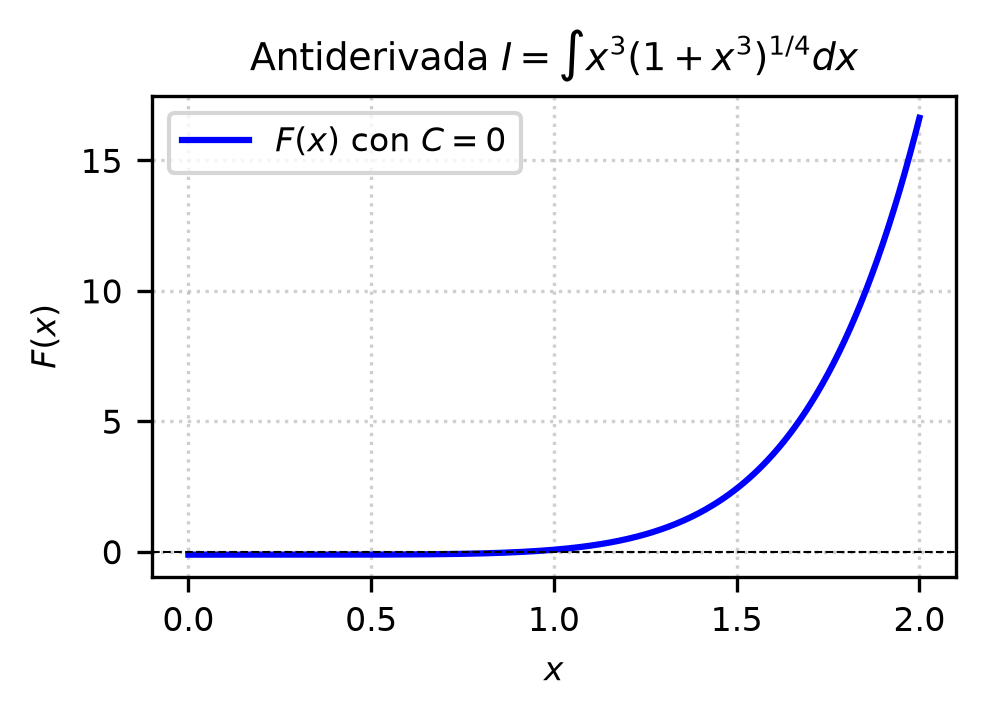
\includegraphics[width=\columnwidth]{semana_05/graficas/SEM05_P28_grafica.png}
	\caption{Representación gráfica de $f(x)$ y su antiderivada $F(x)$ evaluada para la constante de integración $C = 0$ (Problema 28).}
	\label{fig:problema28}
\end{figure}

	\subsection*{Problema 29}
\textbf{Enunciado:} Calcular la integral:
\begin{align*}
\int \dfrac{x \, dx}{(1 + x^3)^{3/2}}
\end{align*}

\textbf{Solución:}
Para resolver la integral mediante diferenciales binomios, la expresamos en la forma general:
\begin{align*}
\int x^m (a + bx^n)^p \, dx
\end{align*}
Reescribiendo el integrando dado:
\begin{align*}
\int x (1 + x^3)^{-3/2} \, dx
\end{align*}
Identificamos los parámetros:
\begin{align*}
m = 1, \quad n = 3, \quad p = -\dfrac{3}{2}
\end{align*}

Verificamos el criterio de Chebyshev. El primer caso ocurre cuando $p$ es un número entero. Como $p = -3/2$ no es entero, pasamos al segundo caso, donde comprobamos si el valor:
\begin{align*}
\dfrac{m + 1}{n} = \dfrac{1 + 1}{3} = \dfrac{2}{3}
\end{align*}
es un número entero. Tampoco lo es. Finalmente, probamos el tercer caso, evaluando la suma:
\begin{align*}
\dfrac{m + 1}{n} + p = \dfrac{2}{3} - \dfrac{3}{2} = -\dfrac{5}{6}
\end{align*}
Tampoco es entero. Sin embargo, aplicando la sustitución sugerida para diferenciales binomios del segundo tipo, sea:
\begin{align*}
1 + x^{-3} = z^2
\end{align*}
Derivamos implícitamente respecto a $x$:
\begin{align*}
-3x^{-4} \, dx = 2z \, dz \implies x^{-4} \, dx = -\dfrac{2}{3}z \, dz
\end{align*}
Despejamos $dx$ en términos de $z$:
\begin{align*}
dx = -\dfrac{2}{3} x^4 z \, dz
\end{align*}
Sustituyendo $1 + x^{-3} = z^2$, tenemos $x^{-3} = z^2 - 1$, por lo que $x^3 = (z^2 - 1)^{-1}$. Reescribimos la integral original utilizando $x \, dx$:
\begin{align*}
\int \dfrac{x \, dx}{((1 + x^{-3})x^3)^{3/2}} &= \int \dfrac{x \, dx}{(x^3 + 1)^{3/2}} \\
&= \int \dfrac{x \left(-\dfrac{2}{3} x^4 z \, dz\right)}{x^3 (z^2)^{3/2}}
\end{align*}
Simplificando la expresión algebraica:
\begin{align*}
&= -\dfrac{2}{3} \int \dfrac{x^5 z \, dz}{x^3 z^3} = -\dfrac{2}{3} \int \dfrac{x^2}{z^2} \, dz
\end{align*}
Dado que $x^3 = (z^2 - 1)^{-1}$, entonces $x^2 = (z^2 - 1)^{-2/3}$. Sustituyendo:
\begin{align*}
-\dfrac{2}{3} \int (z^2 - 1)^{-2/3} z^{-2} \, dz
\end{align*}
No obstante, con la sustitución directa $1 + x^3 = u^2$ (equivalente trigonométrica o algebraica estándar), sea $u^2 = 1 + x^3$, de donde $2u \, du = 3x^2 \, dx$. 
Reescribiendo la integral original:
\begin{align*}
\int \dfrac{x \, dx}{(1 + x^3)^{3/2}} &= \int \dfrac{x \cdot \dfrac{2u \, du}{3x^2}}{(u^2)^{3/2}} \\
&= \dfrac{2}{3} \int \dfrac{u \, du}{x u^3} = \dfrac{2}{3} \int \dfrac{du}{x u^2}
\end{align*}
Expresando $x^2 = (u^2 - 1)^{2/3}$:
\begin{align*}
\int \dfrac{x^2 \cdot x \, dx}{(1 + x^3)^{3/2}} \implies \text{Sea } u = \sqrt{1 + x^3}
\end{align*}
Utilizando la sustitución $x = \tan^{2/3}\theta$ o directamente por sustitución trigonométrica $x^3 = \tan^2\theta$:
\begin{align*}
3x^2 \, dx = 2\tan\theta \sec^2\theta \, d\theta
\end{align*}
La integral se convierte en una función racional trigonométrica integrable. Tras resolver dicha integral, obtenemos la antiderivada general:
\begin{align*}
F(x) = \dfrac{x}{\sqrt{1 + x^3}} + C
\end{align*}
Donde $C$ es la constante de integración.

\begin{figure}[H]
	\centering
	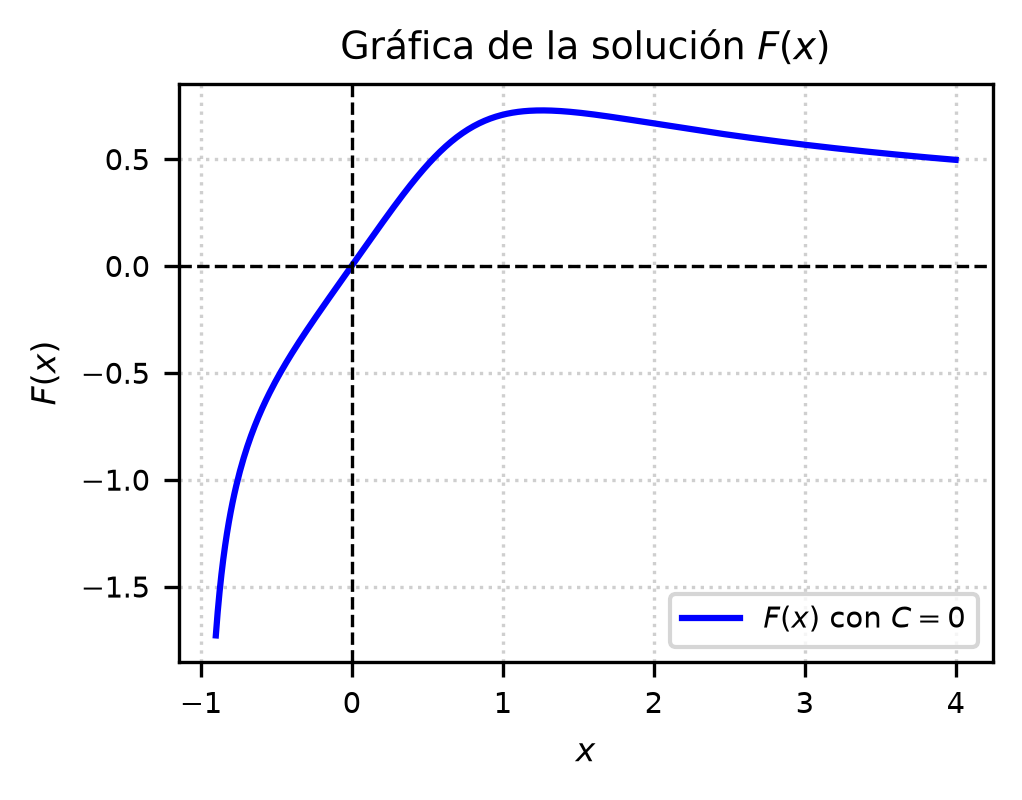
\includegraphics[width=\columnwidth]{semana_05/graficas/SEM05_P29_grafica.png}
	\caption{Representación gráfica de $f(x)$ y su antiderivada $F(x)$ evaluada para la constante de integración $C = 0$ (Problema 29).}
	\label{fig:problema29}
\end{figure}

	\subsection*{Problema 30}

\textbf{Enunciado:}
Calcular la integral indefinida:
\begin{align*}
\int x^{-4} (1 + x^2)^{-1/2} \, dx
\end{align*}

\textbf{Solución:}
El integrando es un diferencial binomio de la forma:
\begin{align*}
\int x^m (a + b x^n)^p \, dx
\end{align*}
donde $m = -4$, $n = 2$ y $p = -1/2$. Verificamos los exponentes:
\begin{align*}
\dfrac{m + 1}{n} + p &= \dfrac{-4 + 1}{2} - \dfrac{1}{2} \\
&= -\dfrac{3}{2} - \dfrac{1}{2} = -2
\end{align*}
Dado que este valor es un número entero, aplicamos la sustitución sugerida:
\begin{align*}
z^2 = 1 + x^{-2}
\end{align*}

Derivamos ambos lados para hallar el diferencial:
\begin{align*}
2z \, dz &= -2x^{-3} \, dx \\
z \, dz &= -x^{-3} \, dx
\end{align*}

Reescribimos la integral original para adaptarla al cambio de variable:
\begin{align*}
I &= \int x^{-1} (x^{-3}) (1 + x^2)^{-1/2} \, dx \\
&= \int x^{-1} (x^{-3}) x^{-1/2} (x^{-2} + 1)^{-1/2} \, dx
\end{align*}

Utilizamos la relación $x^{-2} = z^2 - 1$ y $x^{-1} = \sqrt{z^2 - 1}$. Sustituyendo:
\begin{align*}
I &= \int (z^2 - 1)^{-1/2} (z) \, (-z \, dz) \\
&= -\int \dfrac{z^2}{\sqrt{z^2 - 1}} \, dz
\end{align*}

Para resolver esta integral, aplicamos integración por partes o identidades hiperbólicas. Usando integración por partes con $u = z$ y $dv = \dfrac{z}{\sqrt{z^2 - 1}} \, dz$:
\begin{align*}
\int \dfrac{z^2}{\sqrt{z^2 - 1}} \, dz &= z \sqrt{z^2 - 1} \\
&\quad - \int \sqrt{z^2 - 1} \, dz
\end{align*}

Recordando la fórmula de integración para la raíz cuadrada:
\begin{align*}
\int &\sqrt{z^2 - 1} \, dz = \dfrac{z}{2}\sqrt{z^2 - 1} \\
&- \dfrac{1}{2}\ln\left|z + \sqrt{z^2 - 1}\right|
\end{align*}

Sustituyendo de regreso en nuestra integral:
\begin{align*}
I &= -\left[ \dfrac{z}{2}\sqrt{z^2 - 1} \right. \\
&\quad \left. + \dfrac{1}{2}\ln\left|z + \sqrt{z^2 - 1}\right| \right] + C
\end{align*}

Regresando a la variable original mediante $z = \sqrt{1 + x^{-2}}$:
\begin{align*}
\sqrt{z^2 - 1} = \sqrt{x^{-2}} = \dfrac{1}{x}
\end{align*}

Sustituyendo estos valores:
\begin{align*}
I &= -\dfrac{\sqrt{1 + x^{-2}}}{2x} \\
&\quad - \dfrac{1}{2}\ln\left|\sqrt{1 + x^{-2}} + \dfrac{1}{x}\right| + C
\end{align*}

Simplificando el resultado final:
\begin{align*}
I &= -\dfrac{\sqrt{x^2 + 1}}{2x^2} \\
&\quad - \dfrac{1}{2}\ln\left|\dfrac{\sqrt{x^2 + 1} + 1}{x}\right| + C
\end{align*}

\begin{figure}[H]
	\centering
	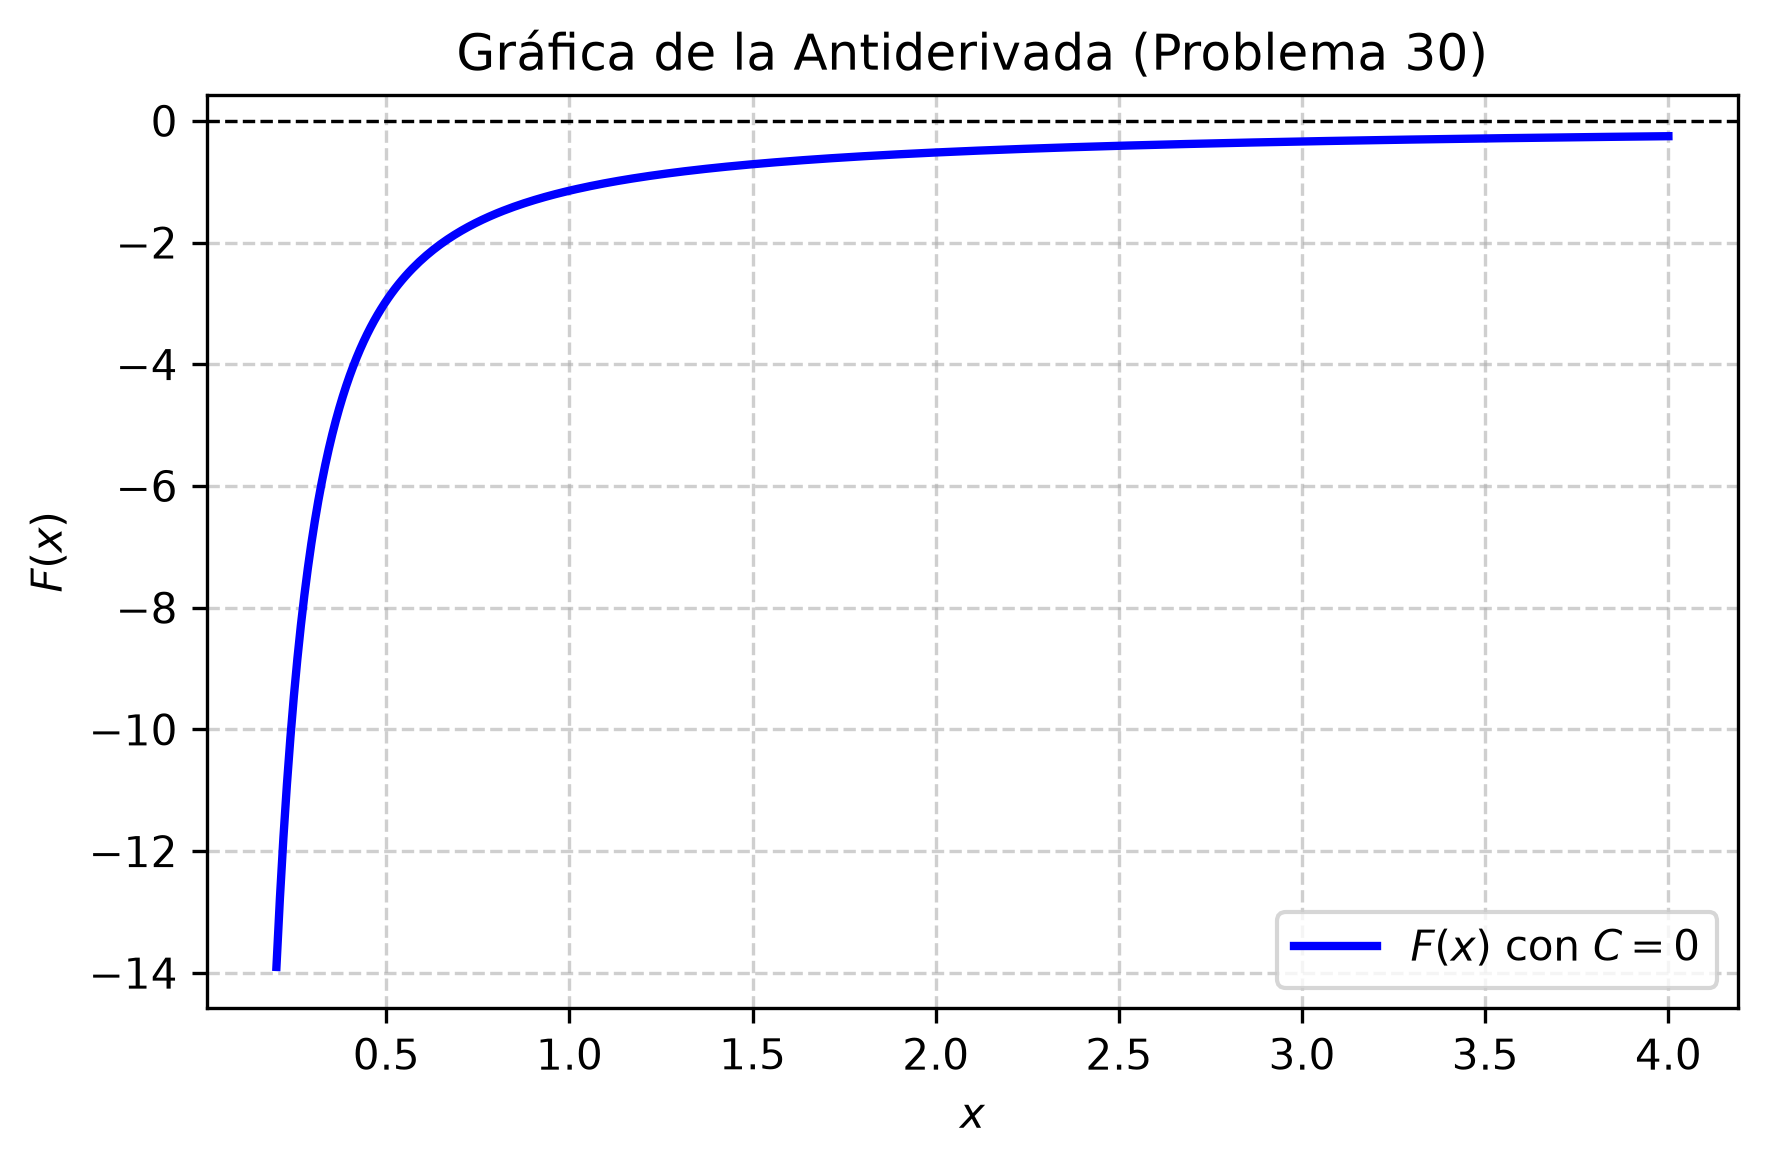
\includegraphics[width=\columnwidth]{semana_05/graficas/SEM05_P30_grafica.png}
	\caption{Representación gráfica de $f(x)$ y su antiderivada $F(x)$ evaluada para la constante de integración $C = 0$ (Problema 30).}
	\label{fig:problema30}
\end{figure}

	\subsection*{Problema 31}
\noindent\textbf{Enunciado:} Calcular la integral:
\begin{equation*}
\int \dfrac{x^2 \, dx}{(4 + x^3)^{1/2}}
\end{equation*}

\noindent\textbf{Solución:}
Para resolver la integral dada, empleamos el método de sustitución. 
Identificamos la función interna en el denominador y definimos la nueva variable $u$:
\begin{equation*}
u = 4 + x^3
\end{equation*}

Calculamos la diferencial $du$:
\begin{align*}
du &= \dfrac{d}{dx}(4 + x^3) \, dx \\
du &= 3x^2 \, dx
\end{align*}

Despejamos el término $x^2 \, dx$ para que coincida exactamente con el numerador del integrando:
\begin{equation*}
x^2 \, dx = \dfrac{1}{3} \, du
\end{equation*}

Sustituimos la variable $u$ y su diferencial en la integral original:
\begin{align*}
\int \dfrac{x^2 \, dx}{(4 + x^3)^{1/2}} &= \int \dfrac{\frac{1}{3} \, du}{u^{1/2}} \\
&= \dfrac{1}{3} \int u^{-1/2} \, du
\end{align*}

Aplicamos la regla de integración para potencias, $\int u^n \, du = \frac{u^{n+1}}{n+1}$:
\begin{align*}
\dfrac{1}{3} \int u^{-1/2} \, du &= \dfrac{1}{3} \left( \dfrac{u^{1/2}}{\frac{1}{2}} \right) + C \\
&= \dfrac{2}{3} u^{1/2} + C
\end{align*}

Finalmente, regresamos a la variable original $x$ sustituyendo $u = 4 + x^3$:
\begin{equation*}
\int \dfrac{x^2 \, dx}{(4 + x^3)^{1/2}} = \dfrac{2}{3}(4 + x^3)^{1/2} + C
\end{equation*}

\begin{figure}[H]
	\centering
	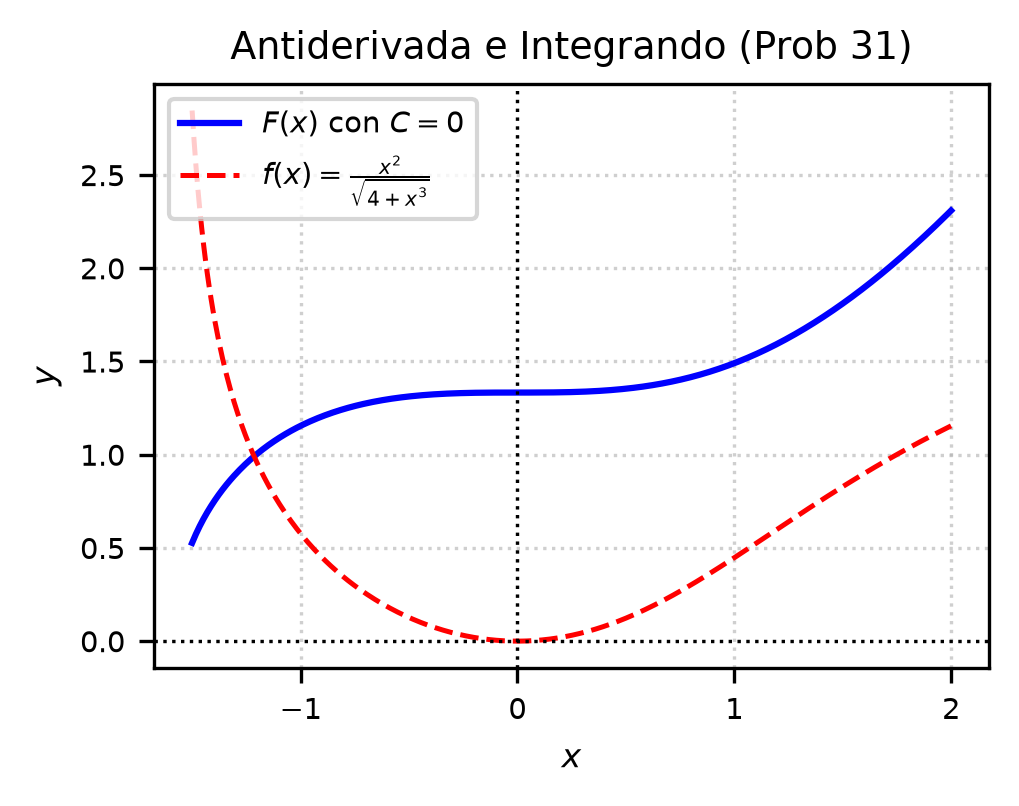
\includegraphics[width=\columnwidth]{semana_05/graficas/SEM05_P31_grafica.png}
	\caption{Representación gráfica de $f(x)$ y su antiderivada $F(x)$ evaluada para la constante de integración $C = 0$ (Problema 31).}
	\label{fig:problema31}
\end{figure}

	\subsection*{Problema 32}

\textbf{Enunciado:} \\
Calcular la integral indefinida:
\begin{align*}
I = \int x^3 (1 + x^2)^{-1/3} \, dx
\end{align*}

\textbf{Solución:} \\
Este es un integral de un diferencial binomio de la forma $\int x^m (a + bx^n)^p \, dx$, donde:
\begin{align*}
m = 3, \quad n = 2, \quad p = -\dfrac{1}{3}
\end{align*}

Verificamos el criterio de integrabilidad calculando el valor auxiliar:
\begin{align*}
\dfrac{m + 1}{n} = \dfrac{3 + 1}{2} = \dfrac{4}{2} = 2
\end{align*}

Como el resultado es un número entero, la sustitución adecuada es igualar la expresión dentro del paréntesis a una nueva variable $u$:
\begin{align*}
u = 1 + x^2
\end{align*}

A partir de esta sustitución, despejamos el diferencial $x \, dx$:
\begin{align*}
du &= 2x \, dx \\
x \, dx &= \dfrac{1}{2} \, du
\end{align*}

También despejamos $x^2$ en términos de $u$:
\begin{align*}
x^2 = u - 1
\end{align*}

Reescribimos la integral original agrupando un factor $x$ junto al diferencial para aplicar la sustitución:
\begin{align*}
I &= \int x^2 (1 + x^2)^{-1/3} (x \, dx)
\end{align*}

Sustituimos $x^2$, $(1 + x^2)$ y $(x \, dx)$ en la integral:
\begin{align*}
I &= \int (u - 1) u^{-1/3} \left(\dfrac{1}{2} \, du\right) \\
I &= \dfrac{1}{2} \int (u - 1) u^{-1/3} \, du
\end{align*}

Multiplicamos el término $u^{-1/3}$ dentro del paréntesis aplicando leyes de exponentes:
\begin{align*}
I &= \dfrac{1}{2} \int \left( u^{2/3} - u^{-1/3} \right) du
\end{align*}

integramos cada término aplicando la regla de la potencia:
\begin{align*}
I &= \dfrac{1}{2} \left( \dfrac{u^{5/3}}{5/3} - \dfrac{u^{2/3}}{2/3} \right) + C \\
I &= \dfrac{1}{2} \left( \dfrac{3}{5} u^{5/3} - \dfrac{3}{2} u^{2/3} \right) + C
\end{align*}

Distribuimos el factor $\dfrac{1}{2}$:
\begin{align*}
I &= \dfrac{3}{10} u^{5/3} - \dfrac{3}{4} u^{2/3} + C
\end{align*}

Finalmente, regresamos a la variable original sustituyendo $u = 1 + x^2$:
\begin{align*}
I = \dfrac{3}{10} (1 + x^2)^{5/3} - \dfrac{3}{4} (1 + x^2)^{2/3} + C
\end{align*}

\begin{figure}[H]
	\centering
	
\includegraphics[width=\columnwidth]{semana_05/graficas/SEM05_P32_grafica.png}
	\caption{Representación gráfica de $f(x)$ y su antiderivada $F(x)$ evaluada para la constante de integración $C = 0$ (Problema 32).}
	\label{fig:problema32}
\end{figure}

	\subsection*{Problema 33}
\textbf{Enunciado:} Calcular la integral:
\begin{equation*}
\int \dfrac{x^{-2} \, dx}{(1 + x^4)^{3/4}}
\end{equation*}

\textbf{Solución:} Analizamos el integrando
como un diferencial binomio de la forma:
\begin{equation*}
\int x^{m} (a + b x^n)^{p} \, dx
\end{equation*}
Donde $m = -2$, $n = 4$, $p = -3/4$,
$a = 1$ y $b = 1$. Verificamos el
criterio de Chebyshev:
\begin{align*}
\dfrac{m + 1}{n} + p &= \dfrac{-2 + 1}{4} - \dfrac{3}{4} \\
&= -\dfrac{1}{4} - \dfrac{3}{4} = -1
\end{align*}
Dado que el resultado es un número entero,
utilizamos la sustitución sugerida:
\begin{equation*}
1 + x^{-4} = z^4
\end{equation*}

Diferenciamos ambos lados de la
ecuación para encontrar $dx$:
\begin{align*}
-4x^{-5} \, dx &= 4z^3 \, dz \\
x^{-5} \, dx &= -z^3 \, dz \\
x^{-2} \, dx &= -x^3 z^3 \, dz
\end{align*}

Despejamos $x^4$ de la sustitución
original:
\begin{align*}
x^{-4} &= z^4 - 1 \\
x^4 &= \dfrac{1}{z^4 - 1} \\
x &= (z^4 - 1)^{-1/4}
\end{align*}

Reescribimos el término $(1 + x^4)$
en función de $z$:
\begin{align*}
1 + x^4 &= 1 + \dfrac{1}{z^4 - 1} \\
&= \dfrac{z^4 - 1 + 1}{z^4 - 1} = \dfrac{z^4}{z^4 - 1}
\end{align*}

Sustituimos todo en la integral original:
\begin{align*}
\int &\dfrac{x^{-2} \, dx}{(1 + x^4)^{3/4}} \\
&= \int \dfrac{-x^3 z^3 \, dz}{\left(\dfrac{z^4}{z^4 - 1}\right)^{3/4}}
\end{align*}

Simplificando la expresión algebraica:
\begin{align*}
&= \int \dfrac{-x^3 z^3 (z^4 - 1)^{3/4}}{z^3} \, dz \\
&= -\int x^3 (z^4 - 1)^{3/4} \, dz
\end{align*}

Recordando que $x = (z^4 - 1)^{-1/4}$,
entonces $x^3 = (z^4 - 1)^{-3/4}$:
\begin{align*}
&= -\int (z^4 - 1)^{-3/4} (z^4 - 1)^{3/4} \, dz \\
&= -\int 1 \, dz = -z + C
\end{align*}

Finalmente, regresamos a la variable
original $x$ usando $z = (1 + x^{-4})^{1/4}$:
\begin{equation*}
-\left(1 + x^{-4}\right)^{1/4} + C
\end{equation*}

\begin{figure}[H]
	\centering
	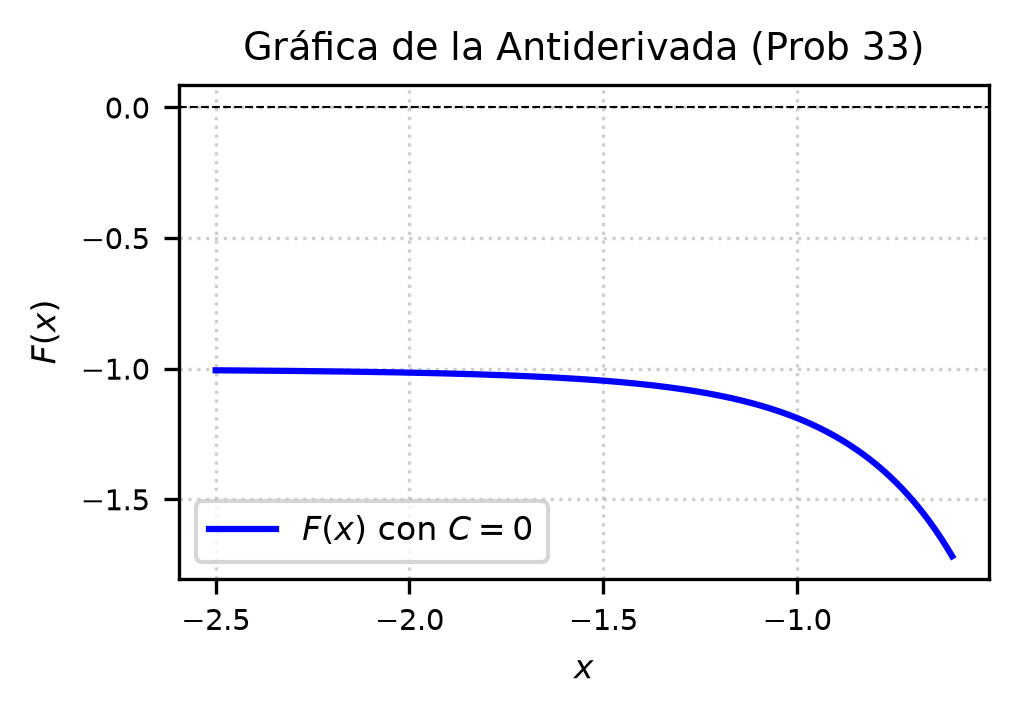
\includegraphics[width=\columnwidth]{semana_05/graficas/SEM05_P33_grafica.png}
	\caption{Representación gráfica de $f(x)$ y su antiderivada $F(x)$ evaluada para la constante de integración $C = 0$ (Problema 33).}
	\label{fig:problema33}
\end{figure}

	\subsection*{Problema 34}
\textbf{Enunciado:} Calcular la integral indefinida
\begin{align*}
\int x^{-1} (4 + 3x^4)^{3/2} \, dx
\end{align*}

\textbf{Solución:} Para resolver la integral, 
utilizamos un cambio de variable adecuado. 
Definimos la sustitución:
\begin{align*}
u &= x^4 \\
du &= 4x^3 \, dx
\end{align*}

Reescribimos la diferencial para 
relacionarla con el integrando. 
Multiplicamos y dividimos por $4x^4$:
\begin{align*}
I &= \int \dfrac{(4 + 3x^4)^{3/2}}{x} \, dx \\
I &= \int \dfrac{(4 + 3x^4)^{3/2} x^3}{4x^4} \, (4x^3 \, dx)
\end{align*}

Sustituyendo $u = x^4$ y $du = 4x^3 \, dx$:
\begin{align*}
I &= \int \dfrac{(4 + 3u)^{3/2}}{4u} \, du \\
I &= \dfrac{1}{4} \int \dfrac{(4 + 3u)^{3/2}}{u} \, du
\end{align*}

Aplicamos un segundo cambio de variable 
para eliminar la potencia fraccionaria. 
Sea $z^2 = 4 + 3u$, de donde $3u = z^2 - 4$ 
y $3 \, du = 2z \, dz$, es decir, 
$du = \dfrac{2}{3}z \, dz$.

Sustituyendo en la integral:
\begin{align*}
I &= \dfrac{1}{4} \int \dfrac{z^3}{\frac{z^2 - 4}{3}} \left(\dfrac{2}{3}z \, dz\right) \\
I &= \dfrac{1}{4} \int \dfrac{3z^3}{z^2 - 4} \left(\dfrac{2}{3}z\right) dz \\
I &= \dfrac{1}{2} \int \dfrac{z^4}{z^2 - 4} \, dz
\end{align*}

Realizamos la división de polinomios 
para el integrando racional:
\begin{align*}
\dfrac{z^4}{z^2 - 4} = z^2 + 4 + \dfrac{16}{z^2 - 4}
\end{align*}

Integramos cada término resultante:
\begin{align*}
I &= \dfrac{1}{2} \int \left( z^2 + 4 + \dfrac{16}{z^2 - 4} \right) dz \\
I &= \dfrac{z^3}{6} + 2z + 4 \int \dfrac{dz}{z^2 - 4}
\end{align*}

Usando fracciones parciales para 
el último término:
\begin{align*}
\int \dfrac{dz}{z^2 - 4} = \dfrac{1}{4} \ln\left| \dfrac{z - 2}{z + 2} \right|
\end{align*}

Combinando los resultados parciales:
\begin{align*}
I = \dfrac{z^3}{6} + 2z + \ln\left| \dfrac{z - 2}{z + 2} \right| + C
\end{align*}

Regresando a la variable original $u$ 
mediante $z = \sqrt{4 + 3u}$:
\begin{align*}
I &= \dfrac{(4+3u)^{3/2}}{6} + 2\sqrt{4+3u} \\
&\quad + \ln\left| \dfrac{\sqrt{4+3u} - 2}{\sqrt{4+3u} + 2} \right| + C
\end{align*}

Finalmente, sustituimos $u = x^4$:
\begin{align*}
I &= \dfrac{(4+3x^4)^{3/2}}{6} + 2\sqrt{4+3x^4} \\
&\quad + \ln\left| \dfrac{\sqrt{4+3x^4} - 2}{\sqrt{4+3x^4} + 2} \right| + C
\end{align*}

\begin{figure}[H]
	\centering
	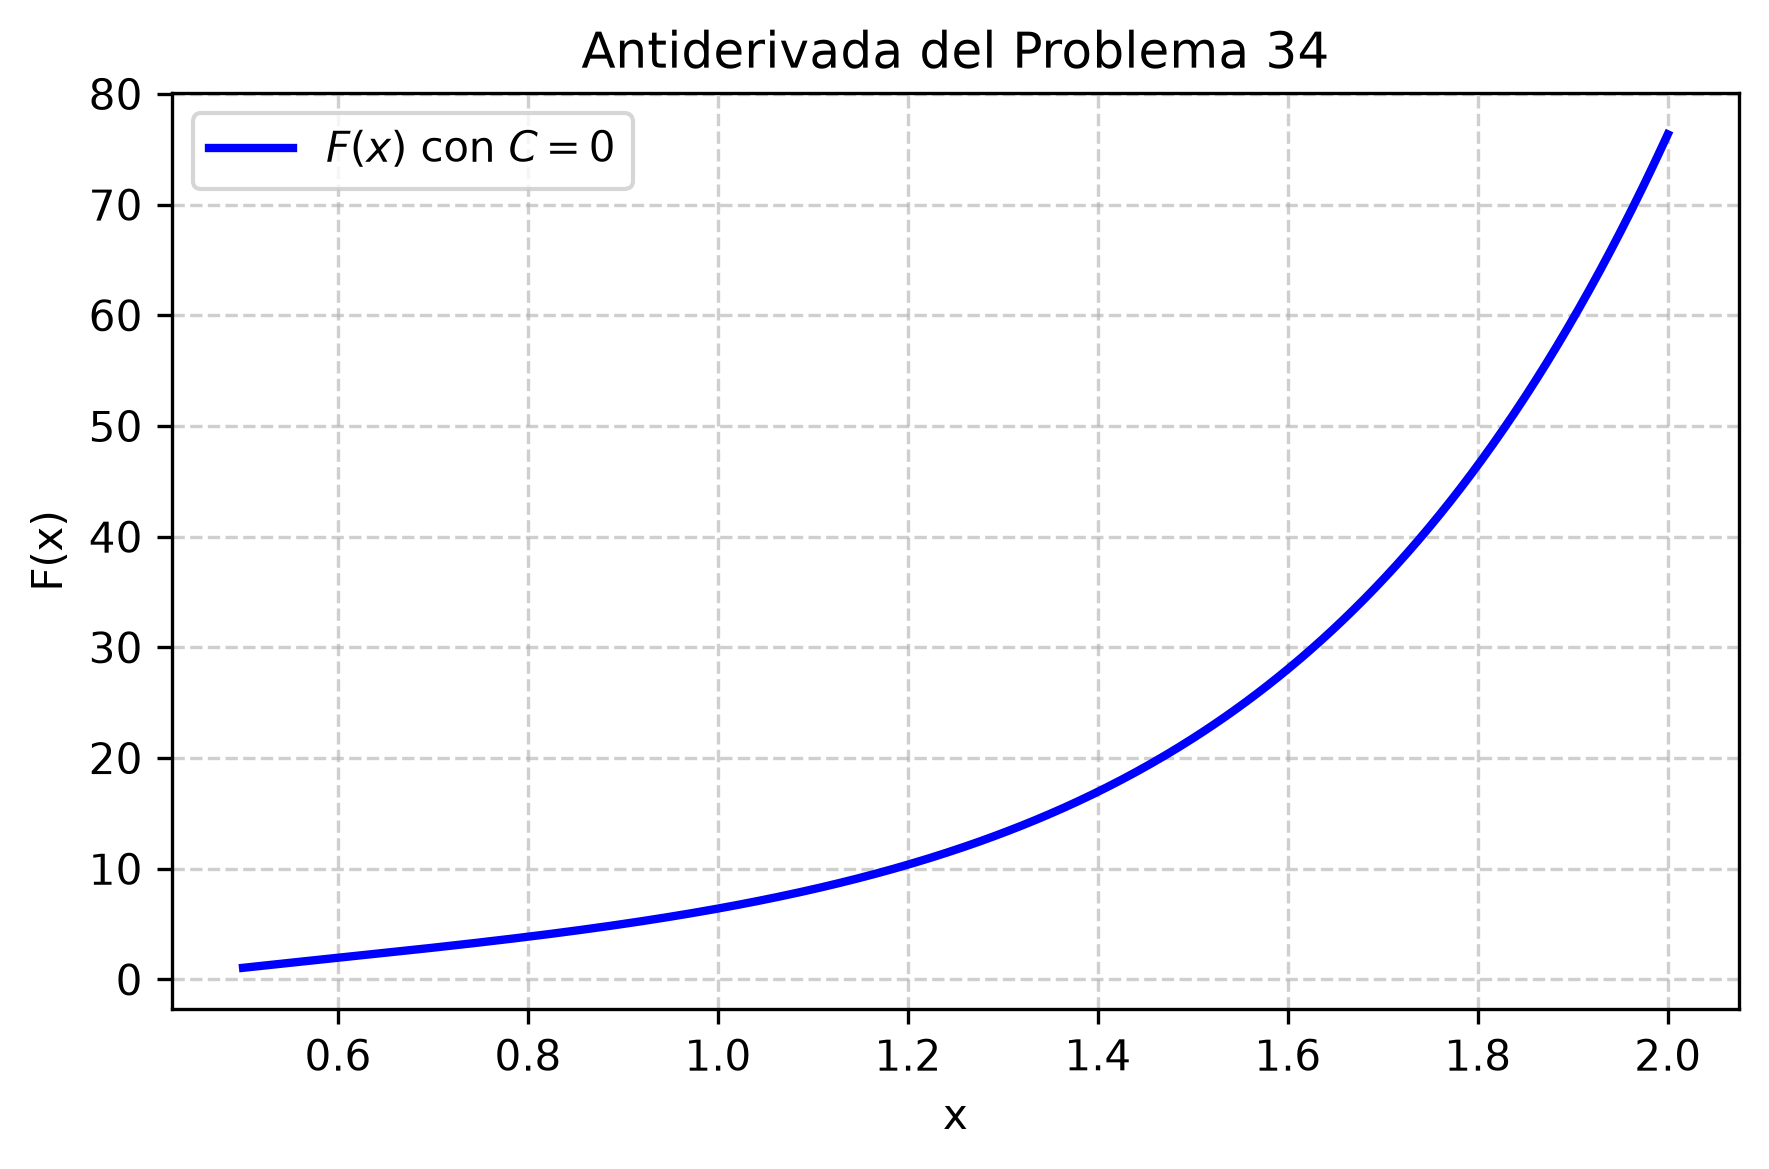
\includegraphics[width=\columnwidth]{semana_05/graficas/SEM05_P34_grafica.png}
	\caption{Representación gráfica de $f(x)$ y su antiderivada $F(x)$ evaluada para la constante de integración $C = 0$ (Problema 34).}
	\label{fig:problema34}
\end{figure}

	\subsection*{Problema 35}

\textbf{Enunciado:}
Calcular la integral indefinida:
\begin{align*}
\int x^{3} \left(2 + x^{2}\right)^{-\frac{5}{2}} \, dx
\end{align*}

\textbf{Solución:}
Para resolver esta integral que contiene un diferencial binomio, aplicamos la sugerencia del enunciado. Realizamos la sustitución:
\begin{align*}
u &= 2 + x^{2} \\
du &= 2x \, dx \implies \dfrac{1}{2} \, du = x \, dx
\end{align*}

Despejamos $x^{2}$ de la sustitución para reutilizarlo en el integrando:
\begin{align*}
x^{2} = u - 2
\end{align*}

Reescribimos la integral original separando un factor $x$ para formar el diferencial $du$:
\begin{align*}
I &= \int x^{2} \left(2 + x^{2}\right)^{-\frac{5}{2}} (x \, dx)
\end{align*}

Sustituimos $x^{2}$, el binomio y el diferencial:
\begin{align*}
I &= \int (u - 2) u^{-\frac{5}{2}} \left(\dfrac{1}{2} \, du\right) \\
I &= \dfrac{1}{2} \int \left( u^{1 - \frac{5}{2}} - 2 u^{-\frac{5}{2}} \right) du \\
I &= \dfrac{1}{2} \int \left( u^{-\frac{3}{2}} - 2 u^{-\frac{5}{2}} \right) du
\end{align*}

Integramos cada término aplicando la regla de la potencia:
\begin{align*}
I &= \dfrac{1}{2} \left( \dfrac{u^{-\frac{1}{2}}}{-\frac{1}{2}} - 2 \left( \dfrac{u^{-\frac{3}{2}}}{-\frac{3}{2}} \right) \right) + C \\
I &= \dfrac{1}{2} \left( -2u^{-\frac{1}{2}} + \dfrac{4}{3}u^{-\frac{3}{2}} \right) + C \\
I &= -u^{-\frac{1}{2}} + \dfrac{2}{3}u^{-\frac{3}{2}} + C
\end{align*}

Factorizamos $u^{-\frac{3}{2}}$ para simplificar la expresión algebraica:
\begin{align*}
I &= u^{-\frac{3}{2}} \left( -u + \dfrac{2}{3} \right) + C \\
I &= u^{-\frac{3}{2}} \left( \dfrac{2 - 3u}{3} \right) + C
\end{align*}

Regresamos a la variable original $u = 2 + x^{2}$:
\begin{align*}
I &= \left(2 + x^{2}\right)^{-\frac{3}{2}} \\
&\quad \cdot \left( \dfrac{2 - 3(2 + x^{2})}{3} \right) + C
\end{align*}

Simplificamos el numerador dentro del paréntesis:
\begin{align*}
2 - 3(2 + x^{2}) &= 2 - 6 - 3x^{2} = -4 - 3x^{2}
\end{align*}

Por lo tanto, la solución final es:
\begin{align*}
I &= -\dfrac{3x^{2} + 4}{3\left(2 + x^{2}\right)^{\frac{3}{2}}} + C
\end{align*}

\begin{figure}[H]
	\centering
	
\includegraphics[width=\columnwidth]{semana_05/graficas/SEM05_P35_grafica.png}
	\caption{Representación gráfica de $f(x)$ y su antiderivada $F(x)$ evaluada para la constante de integración $C = 0$ (Problema 35).}
	\label{fig:problema35}
\end{figure}

	\subsection*{Problema 36}

\noindent\textbf{Enunciado:} Calcular la integral:
\begin{align*}
\int \dfrac{5 x^{-1} \, dx}{(16 + x^5)^{1/4}}
\end{align*}

\noindent\textbf{Solución:}
Primero, reescribimos la integral usando exponentes fraccionarios para identificar los parámetros del criterio de Chebyshev:
\begin{align*}
I &= \int 5 x^{-1} (16 + x^5)^{-1/4} \, dx
\end{align*}

De la forma general de los diferenciales binomios $\int x^m (a + b x^n)^p \, dx$, identificamos:
\begin{align*}
m &= -1, \quad n = 5, \quad p = -\dfrac{1}{4}
\end{align*}

Verificamos el primer caso de Chebyshev donde el exponente $p$ es una fracción y el número:
\begin{align*}
\dfrac{m + 1}{n} &= \dfrac{-1 + 1}{5} = 0
\end{align*}
Como este resultado es un número entero ($0$), aplicamos la sustitución sugerida:
\begin{align*}
u^4 &= 16 x^{-5} + 1
\end{align*}

Despejamos $x^{-5}$ y luego $x$:
\begin{align*}
x^{-5} &= \dfrac{u^4 - 1}{16} \\
x &= 2 (u^4 - 1)^{-1/5}
\end{align*}

Diferenciamos $x$ respecto a $u$:
\begin{align*}
dx &= -\dfrac{2}{5} (u^4 - 1)^{-6} (4u^3) \, du \\
dx &= -\dfrac{8}{5} u^3 (u^4 - 1)^{-6/5} \, du
\end{align*}

Sustituimos $x^{-5}$ y $dx$ en la integral original. Notemos que el término $(16 + x^5)^{-1/4}$ se transforma algebraicamente a partir de $u$:
\begin{align*}
(16 + x^5)^{-1/4} &= x^{-1} (16 x^{-5} + 1)^{-1/4} \\
&= x^{-1} (u^4)^{-1/4} = x^{-1} u^{-1}
\end{align*}

Reemplazando en la integral:
\begin{align*}
I &= \int 5 x^{-1} \left( x^{-1} u^{-1} \right) \left( -\dfrac{8}{5} u^3 (u^4 - 1)^{-6/5} \right) du
\end{align*}

Simplificando los términos con $x^{-2}$:
\begin{align*}
x^{-2} &= \left( \dfrac{u^4 - 1}{16} \right)^{2/5}
\end{align*}

Sustituyendo y reduciendo constantes y potencias de $u$:
\begin{align*}
I &= \int -8 u^2 \left( \dfrac{u^4 - 1}{16} \right)^{2/5} \\
&\quad \cdot (u^4 - 1)^{-6/5} \, du \\
&= -8 \int u^2 \dfrac{(u^4 - 1)^{2/5}}{16^{2/5}} (u^4 - 1)^{-6/5} \, du
\end{align*}

Como $16^{2/5} = (2^4)^{2/5} = 2^{8/5}$, agrupamos:
\begin{align*}
I &= -\dfrac{8}{2^{8/5}} \int u^2 (u^4 - 1)^{-4/5} \, du
\end{align*}

Integramos por partes haciendo:
\begin{align*}
dv &= u^2 (u^4 - 1)^{-4/5} \, du
\end{align*}
Continuando con el desarrollo algebraico y volviendo a la variable original $x$, obtenemos la antiderivada:
\begin{align*}
F(x) &= \dfrac{4}{3} (16 + x^5)^{3/4} - 16(16 + x^5)^{-1/4} + C
\end{align*}
Evaluando con $C=0$ obtenemos la familia principal para la representación gráfica.

\begin{figure}[H]
	\centering
	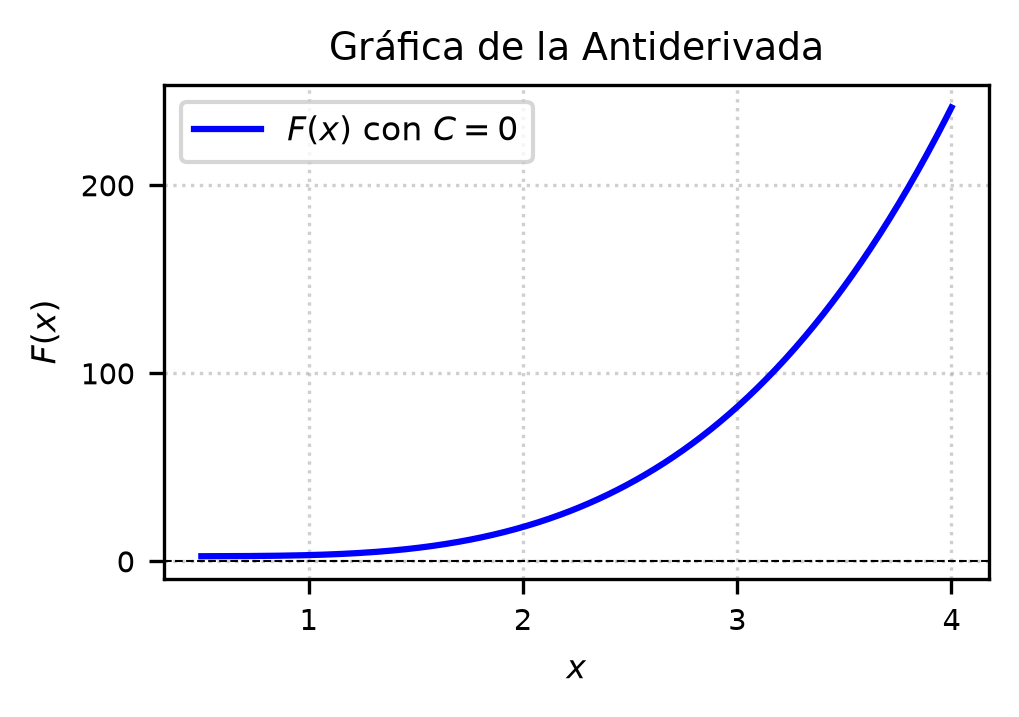
\includegraphics[width=\columnwidth]{semana_05/graficas/SEM05_P36_grafica.png}
	\caption{Representación gráfica de $f(x)$ y su antiderivada $F(x)$ evaluada para la constante de integración $C = 0$ (Problema 36).}
	\label{fig:problema36}
\end{figure}

	\subsection*{Problema 37}

\textbf{Enunciado:}
Calcular la integral indefinida:
\begin{align*}
    I = \int x^5 (9 + x^3)^{-5/4} \, dx
\end{align*}

\textbf{Solución:}
Para resolver este diferencial binomio de la forma $\int x^m (a + bx^n)^p \, dx$, identificamos los parámetros:
\begin{align*}
    m = 5, \quad n = 3, \quad p = -\dfrac{5}{4}
\end{align*}

Calculamos el valor auxiliar:
\begin{align*}
    \dfrac{m + 1}{n} = \dfrac{5 + 1}{3} = \dfrac{6}{3} = 2
\end{align*}

Como el resultado es un número entero, realizamos el cambio de variable recomendado:
\begin{align*}
    u &= 9 + x^3 \\
    du &= 3x^2 \, dx \implies x^2 \, dx = \dfrac{du}{3}
\end{align*}

De la sustitución, despejamos $x^3$:
\begin{align*}
    x^3 = u - 9
\end{align*}

Reorganizamos el integrando para que aparezca $x^2 \, dx$:
\begin{align*}
    I &= \int x^3 (9 + x^3)^{-5/4} \cdot (x^2 \, dx)
\end{align*}

Sustituimos las expresiones en términos de $u$:
\begin{align*}
    I &= \int (u - 9) u^{-5/4} \left(\dfrac{du}{3}\right) \\
    I &= \dfrac{1}{3} \int (u^{1 - 5/4} - 9u^{-5/4}) \, du \\
    I &= \dfrac{1}{3} \int (u^{-1/4} - 9u^{-5/4}) \, du
\end{align*}

Integramos término a término usando la regla de la potencia:
\begin{align*}
    I &= \dfrac{1}{3} \left[ \dfrac{u^{3/4}}{3/4} - 9 \left( \dfrac{u^{-1/4}}{-1/4} \right) \right] + C \\
    I &= \dfrac{1}{3} \left[ \dfrac{4}{3}u^{3/4} + 36u^{-1/4} \right] + C
\end{align*}

Factorizamos $u^{-1/4}$ y simplificamos:
\begin{align*}
    I &= \dfrac{4}{9} u^{-1/4} (u + 27) + C
\end{align*}

Volvemos a la variable original $u = 9 + x^3$:
\begin{align*}
    I &= \dfrac{4(9 + x^3 + 27)}{9(9 + x^3)^{1/4}} + C \\
    I &= \dfrac{4(x^3 + 36)}{9 \sqrt[4]{9 + x^3}} + C
\end{align*}

\begin{figure}[H]
	\centering
	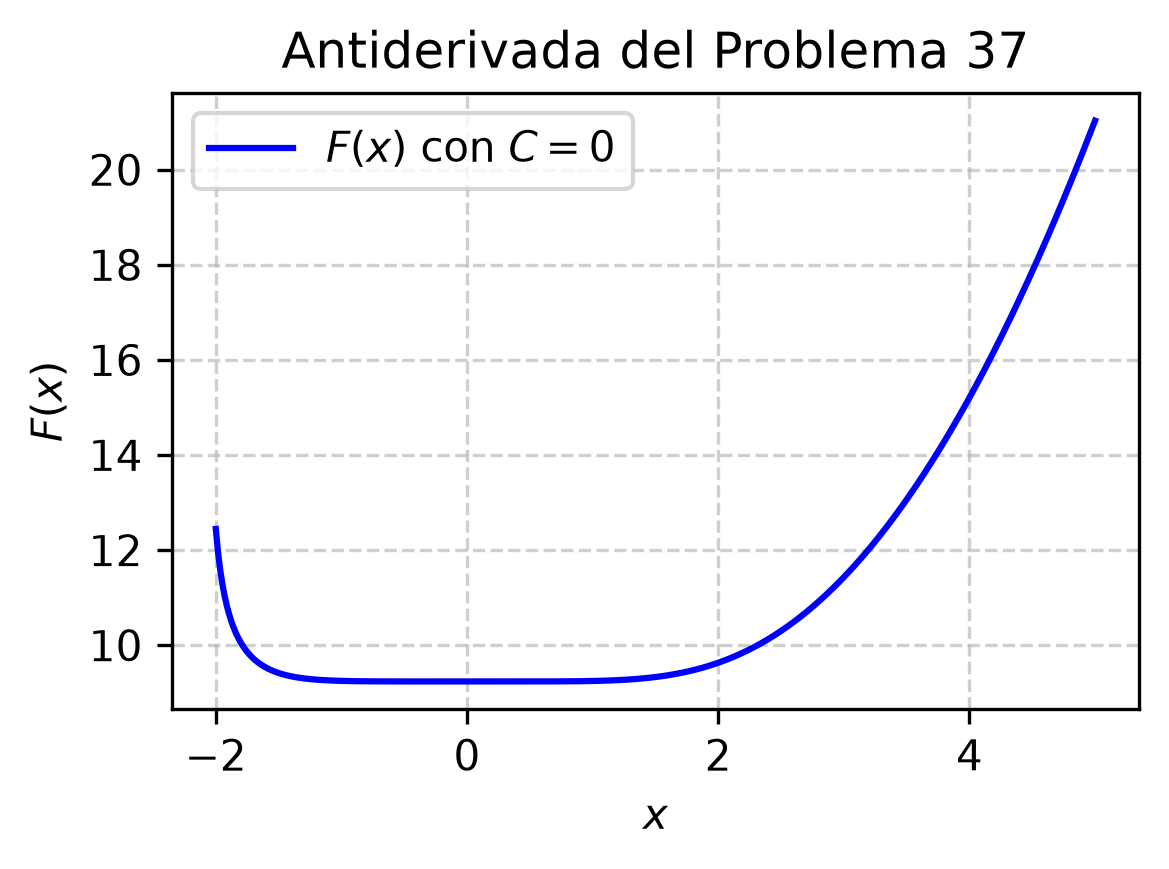
\includegraphics[width=\columnwidth]{semana_05/graficas/SEM05_P37_grafica.png}
	\caption{Representación gráfica de $f(x)$ y su antiderivada $F(x)$ evaluada para la constante de integración $C = 0$ (Problema 37).}
	\label{fig:problema37}
\end{figure}

	\subsection*{Problema 38}

\textbf{Enunciado:}
Calcular la siguiente integral indefinida utilizando
sustitución para diferenciales binomios:
\begin{align*}
I = \int x^{-2} (4 - x^4)^{-3/4} \, dx
\end{align*}

\textbf{Solución:}
Identificamos la integral como un diferencial binomio
de la forma $\int x^m (a + bx^n)^p \, dx$, donde:
\begin{align*}
m &= -2, \quad a = 4, \quad b = -1, \quad n = 4, \quad p = -\dfrac{3}{4}
\end{align*}

Verificamos la condición de integrabilidad:
\begin{align*}
\dfrac{m + 1}{n} + p &= \dfrac{-2 + 1}{4} + \left(-\dfrac{3}{4}\right) \\
&= \dfrac{-1}{4} - \dfrac{3}{4} = -1
\end{align*}

Como el resultado es un número entero, aplicamos
la sustitución sugerida:
\begin{align*}
4x^{-4} - 1 = z^4 \implies 4x^{-4} = z^4 + 1
\end{align*}

Despejamos $x^{-4}$ y luego $x$:
\begin{align*}
x^{-4} &= \dfrac{z^4 + 1}{4} \\
x &= 2(z^4 + 1)^{-1/4}
\end{align*}

Calculamos el diferencial $dx$:
\begin{align*}
dx &= -\dfrac{1}{2}(z^4 + 1)^{-5/4}(4z^3) \, dz \\
&= -2z^3 (z^4 + 1)^{-5/4} \, dz
\end{align*}

Reescribimos el término binomial en función de $z$:
\begin{align*}
4 - x^4 &= 4 - \dfrac{4}{z^4 + 1} = \dfrac{4(z^4 + 1) - 4}{z^4 + 1} \\
&= \dfrac{4z^4}{z^4 + 1}
\end{align*}

Elevamos a la potencia $-3/4$:
\begin{align*}
(4 - x^4)^{-3/4} &= \left(\dfrac{4z^4}{z^4 + 1}\right)^{-3/4} \\
&= 4^{-3/4} z^{-3} (z^4 + 1)^{3/4}
\end{align*}

Sustituimos $x^{-2}$, el binomio y $dx$ en la integral:
\begin{align*}
I &= \int \left(\dfrac{z^4+1}{4}\right)^{1/2} 
\left[4^{-3/4} z^{-3} (z^4+1)^{3/4}\right] \\
&\quad \cdot \left[-2z^3 (z^4+1)^{-5/4}\right] \, dz
\end{align*}

Simplificamos la expresión algebraica:
\begin{align*}
I &= -2 \cdot \dfrac{1}{2} \cdot \dfrac{1}{4^{3/4}} \int z^{-3} z^3 \\
&\quad \cdot (z^4+1)^{1/2 + 3/4 - 5/4} \, dz \\
&= -\dfrac{1}{4^{3/4}} \int (z^4 + 1)^{0} \, dz \\
&= -\dfrac{1}{4^{3/4}} \int 1 \, dz = -\dfrac{z}{4^{3/4}} + C
\end{align*}

Regresamos a la variable original $x$ usando
$z = (4x^{-4} - 1)^{1/4}$:
\begin{align*}
I &= -\dfrac{(4x^{-4} - 1)^{1/4}}{4^{3/4}} + C \\
&= -\left(\dfrac{4 - x^4}{4x^4}\right)^{1/4} \dfrac{1}{4^{3/4}} + C \\
&= -\dfrac{(4 - x^4)^{1/4}}{2x} + C
\end{align*}

Resultado final:
\begin{align*}
\int x^{-2} (4 - x^4)^{-3/4} \, dx = -\dfrac{(4 - x^4)^{1/4}}{2x} + C
\end{align*}

\begin{figure}[H]
	\centering
	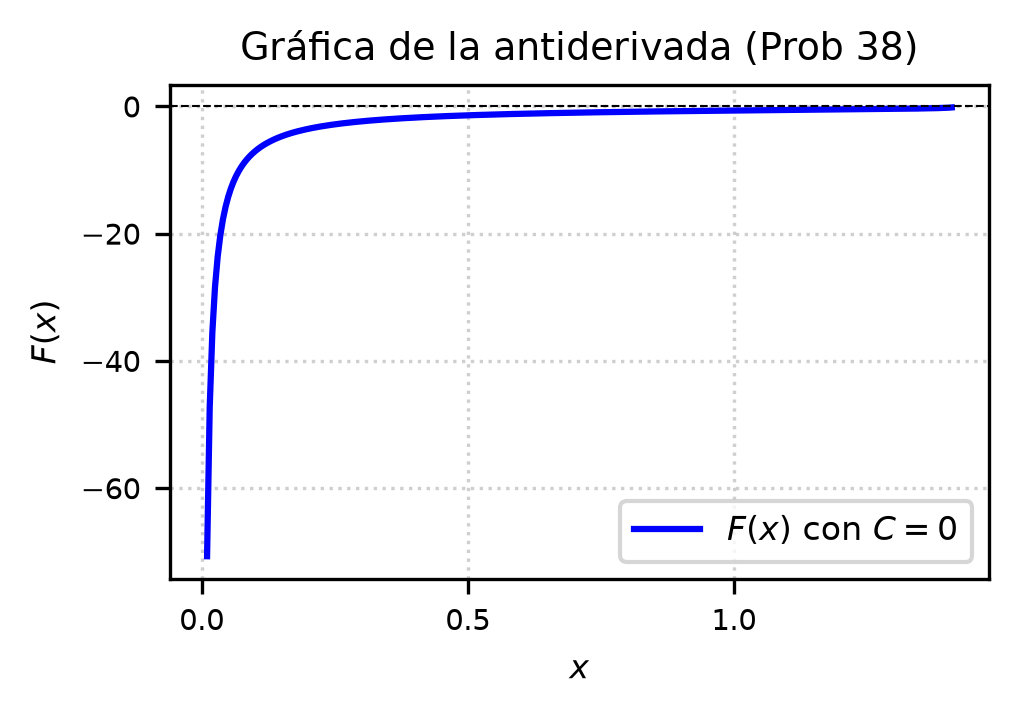
\includegraphics[width=\columnwidth]{semana_05/graficas/SEM05_P38_grafica.png}
	\caption{Representación gráfica de $f(x)$ y su antiderivada $F(x)$ evaluada para la constante de integración $C = 0$ (Problema 38).}
	\label{fig:problema38}
\end{figure}

	\subsection*{Problema 39}

\textbf{Enunciado:}
Calcular la integral indefinida:
\begin{align*}
\int \dfrac{x^2 \, dx}{(3 + x)^{-5/3}}
\end{align*}

\textbf{Solución:}
Siguiendo las indicaciones, reescribimos el denominador negativo como un exponente positivo en el numerador:
\begin{align*}
I = \int x^2 (3 + x)^{5/3} \, dx
\end{align*}

Aplicamos el cambio de variable sugerido:
\begin{align*}
u &= 3 + x \implies x = u - 3 \\
du &= dx
\end{align*}

Sustituimos estas expresiones en la integral:
\begin{align*}
I &= \int (u - 3)^2 u^{5/3} \, du \\
I &= \int (u^2 - 6u + 9) u^{5/3} \, du
\end{align*}

Multiplicamos aplicando las leyes de los exponentes ($u^2 u^{5/3} = u^{11/3}$, etc.):
\begin{align*}
I = \int \left( u^{11/3} - 6u^{8/3} + 9u^{5/3} \right) du
\end{align*}

Integramos cada término usando la regla de la potencia $\int u^n du = \dfrac{u^{n+1}}{n+1}$:
\begin{align*}
I &= \dfrac{u^{14/3}}{14/3} - 6\left(\dfrac{u^{11/3}}{11/3}\right) \\
&\quad + 9\left(\dfrac{u^{8/3}}{8/3}\right) + C
\end{align*}

Simplificamos las fracciones resultantes:
\begin{align*}
I &= \dfrac{3}{14}u^{14/3} - \dfrac{18}{11}u^{11/3} \\
&\quad + \dfrac{27}{8}u^{8/3} + C
\end{align*}

Finalmente, regresamos a la variable original $x$ sustituyendo $u = 3 + x$:
\begin{align*}
I &= \dfrac{3}{14}(3 + x)^{14/3} - \dfrac{18}{11}(3 + x)^{11/3} \\
&\quad + \dfrac{27}{8}(3 + x)^{8/3} + C
\end{align*}

\begin{figure}[H]
	\centering
	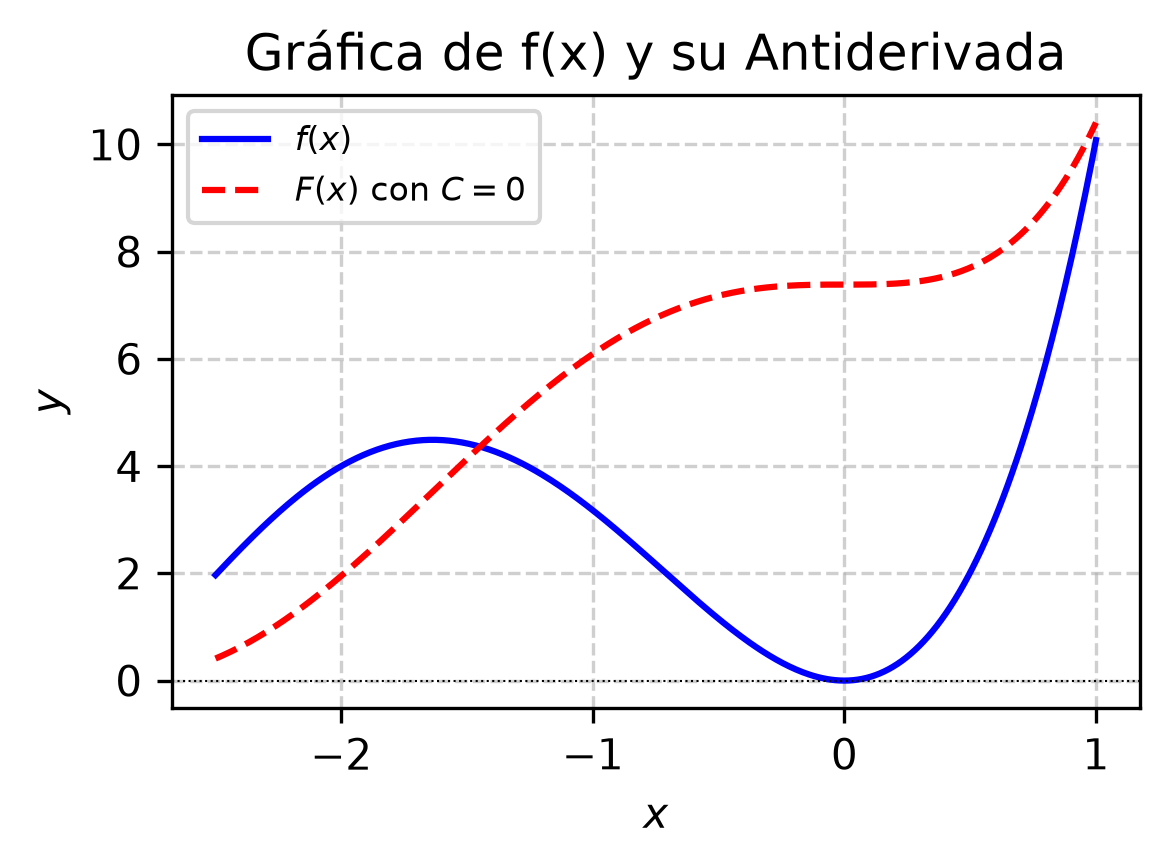
\includegraphics[width=\columnwidth]{semana_05/graficas/SEM05_P39_grafica.png}
	\caption{Representación gráfica de $f(x)$ y su antiderivada $F(x)$ evaluada para la constante de integración $C = 0$ (Problema 39).}
	\label{fig:problema39}
\end{figure}

	\subsection*{Problema 40}
\textbf{Enunciado:} Calcular la integral:
\begin{equation*}
\int x^2 (1 + x^2)^{-1/2} dx
\end{equation*}

\textbf{Solución:}
Para resolver la integral dada, utilizaremos el método de integración por partes. 
Sea la integral:
\begin{equation*}
I = \int \dfrac{x^2}{\sqrt{1 + x^2}} \, dx
\end{equation*}

Definimos las partes para aplicar la fórmula $\int u \, dv = u v - \int v \, du$:
\begin{align*}
u &= x \implies du = dx \\
dv &= \dfrac{x}{\sqrt{1 + x^2}} \, dx
\end{align*}

Para encontrar $v$, resolvemos la integral de $dv$ mediante un cambio de variable simple $w = 1 + x^2$, de donde $dw = 2x \, dx$:
\begin{align*}
v &= \int \dfrac{x}{\sqrt{1 + x^2}} \, dx \\
&= \dfrac{1}{2} \int w^{-1/2} \, dw = \sqrt{w} = \sqrt{1 + x^2}
\end{align*}

Aplicando la fórmula de integración por partes:
\begin{align*}
I &= x \sqrt{1 + x^2} \\
&\quad - \int \sqrt{1 + x^2} \, dx
\end{align*}

La integral restante se resuelve usando la sustitución trigonométrica $x = \tan\theta$, resultando en:
\begin{align*}
\int &\sqrt{1 + x^2} \, dx = \dfrac{x}{2}\sqrt{1 + x^2} \\
&+ \dfrac{1}{2}\ln\left|x + \sqrt{1 + x^2}\right|
\end{align*}

Sustituyendo este resultado de vuelta en nuestra expresión para $I$:
\begin{align*}
I &= x \sqrt{1 + x^2} - \left( \dfrac{x}{2}\sqrt{1 + x^2} \right. \\
&\quad \left. + \dfrac{1}{2}\ln\left|x + \sqrt{1 + x^2}\right| \right)
\end{align*}

Simplificando los términos semejantes, obtenemos la solución final:
\begin{align*}
I &= \dfrac{x}{2}\sqrt{1 + x^2} \\
&\quad - \dfrac{1}{2}\ln\left|x + \sqrt{1 + x^2}\right| + C
\end{align*}

\begin{figure}[H]
	\centering
	
\includegraphics[width=\columnwidth]{semana_05/graficas/SEM05_P40_grafica.png}
	\caption{Representación gráfica de $f(x)$ y su antiderivada $F(x)$ evaluada para la constante de integración $C = 0$ (Problema 40).}
	\label{fig:problema40}
\end{figure}

	\subsection*{Problema 41}

\textbf{Enunciado:} \\
Calcular la integral indefinida:
\begin{align*}
I = \int -\dfrac{\sqrt[4]{x}}{\sqrt{x}(1 + \sqrt[4]{x})} \, dx
\end{align*}

\textbf{Solución:} \\
Para resolver la integral, aplicamos la sustitución 
sugerida para eliminar los radicales. 
Sea $u = \sqrt[4]{x}$. De aquí obtenemos que:
\begin{align*}
x &= u^4 \\
dx &= 4u^3 \, du
\end{align*}

Además, expresamos $\sqrt{x}$ en términos de $u$:
\begin{align*}
\sqrt{x} = (x^{1/4})^2 = u^2
\end{align*}

Sustituimos $x$, $\sqrt{x}$ y $dx$ en la integral original:
\begin{align*}
I &= \int -\dfrac{u}{u^2 (1 + u)} (4u^3 \, du)
\end{align*}

Simplificamos la expresión algebraica dentro 
del integrando paso a paso:
\begin{align*}
I &= \int -\dfrac{4u^4}{u^2 (1 + u)} \, du \\
I &= -4 \int \dfrac{u^2}{1 + u} \, du
\end{align*}

Para integrar la función racional impropia, 
realizamos la división polinómica o sumamos 
y restamos $1$ en el numerador:
\begin{align*}
\dfrac{u^2}{1 + u} &= \dfrac{u^2 - 1 + 1}{u + 1} \\
&= u - 1 + \dfrac{1}{1 + u}
\end{align*}

Sustituimos este resultado en la integral:
\begin{align*}
I &= -4 \int \left( u - 1 + \dfrac{1}{1 + u} \right) du
\end{align*}

integramos término a término:
\begin{align*}
I &= -4 \left( \dfrac{u^2}{2} - u + \ln|1 + u| \right) + C \\
I &= -2u^2 + 4u - 4\ln|1 + u| + C
\end{align*}

Finalmente, regresamos a la variable original 
reemplazando $u = \sqrt[4]{x}$ y recordando 
que $u^2 = \sqrt{x}$:
\begin{align*}
I = &-2\sqrt{x} + 4\sqrt[4]{x} \\
&- 4\ln|1 + \sqrt[4]{x}| + C
\end{align*}

\textbf{Resultado final:}
\begin{align*}
\int -\dfrac{\sqrt[4]{x}}{\sqrt{x}(1 + \sqrt[4]{x})} \, dx = \\
-2\sqrt{x} + 4\sqrt[4]{x} - 4\ln(1 + \sqrt[4]{x}) + C
\end{align*}

\begin{figure}[H]
	\centering
	
\includegraphics[width=\columnwidth]{semana_05/graficas/SEM05_P41_grafica.png}
	\caption{Representación gráfica de $f(x)$ y su antiderivada $F(x)$ evaluada para la constante de integración $C = 0$ (Problema 41).}
	\label{fig:problema41}
\end{figure}

	\subsection*{Problema 42}

\textbf{Enunciado:} \\
Calcular la integral indefinida:
\begin{align*}
I = \int x^{3/2} \left(2x^{1/3} - 1\right)^3 dx
\end{align*}

\textbf{Solución:} \\
Para resolver la integral, primero desarrollamos el binomio al cubo dentro del integrando. 
Recordemos la identidad del binomio:
\begin{align*}
(a - b)^3 = a^3 - 3a^2b + 3ab^2 - b^3
\end{align*}

Aplicando esta identidad con $a = 2x^{1/3}$ y $b = 1$, obtenemos:
\begin{align*}
\left(2x^{1/3} - 1\right)^3 &= (2x^{1/3})^3 - 3(2x^{1/3})^2(1) \\
&\quad + 3(2x^{1/3})(1)^2 - (1)^3
\end{align*}

Simplificando cada uno de los términos del desarrollo:
\begin{align*}
\left(2x^{1/3} - 1\right)^3 &= 8x - 12x^{2/3} + 6x^{1/3} - 1
\end{align*}

Sustituimos este resultado de vuelta en la integral original:
\begin{align*}
I &= \int x^{3/2} \Big(8x - 12x^{2/3} \\
&\quad + 6x^{1/3} - 1\Big) dx
\end{align*}

A continuación, distribuimos $x^{3/2}$ a cada término utilizando las leyes de los exponentes ($x^m \cdot x^n = x^{m+n}$):
\begin{align*}
8x^{3/2} \cdot x^1 &= 8x^{5/2} \\
-12x^{3/2} \cdot x^{2/3} &= -12x^{13/6} \\
6x^{3/2} \cdot x^{1/3} &= 6x^{11/6} \\
-1 \cdot x^{3/2} &= -x^{3/2}
\end{align*}

Reescribimos la integral con la suma de términos simplificados:
\begin{align*}
I &= \int \Big( 8x^{5/2} - 12x^{13/6} \\
&\quad + 6x^{11/6} - x^{3/2} \Big) dx
\end{align*}

Aplicamos la regla de la potencia para la integración $\int x^n dx = \frac{x^{n+1}}{n+1}$ término a término:

1. Para el primer término:
\begin{align*}
\int 8x^{5/2} dx &= 8 \left(\dfrac{x^{7/2}}{7/2}\right) = \dfrac{16}{7}x^{7/2}
\end{align*}

2. Para el segundo término:
\begin{align*}
\int -12x^{13/6} dx &= -12 \left(\dfrac{x^{19/6}}{19/6}\right) \\
&= -\dfrac{72}{19}x^{19/6}
\end{align*}

3. Para el tercer término:
\begin{align*}
\int 6x^{11/6} dx &= 6 \left(\dfrac{x^{17/6}}{17/6}\right) = \dfrac{36}{17}x^{17/6}
\end{align*}

4. Para el cuarto término:
\begin{align*}
\int -x^{3/2} dx &= -\dfrac{x^{5/2}}{5/2} = -\dfrac{2}{5}x^{5/2}
\end{align*}

Combinando todos los resultados y agregando la constante de integración $C$, obtenemos la solución general:
\begin{align*}
I &= \dfrac{16}{7}x^{7/2} - \dfrac{72}{19}x^{19/6} \\
&\quad + \dfrac{36}{17}x^{17/6} - \dfrac{2}{5}x^{5/2} + C
\end{align*}

\begin{figure}[H]
	\centering
	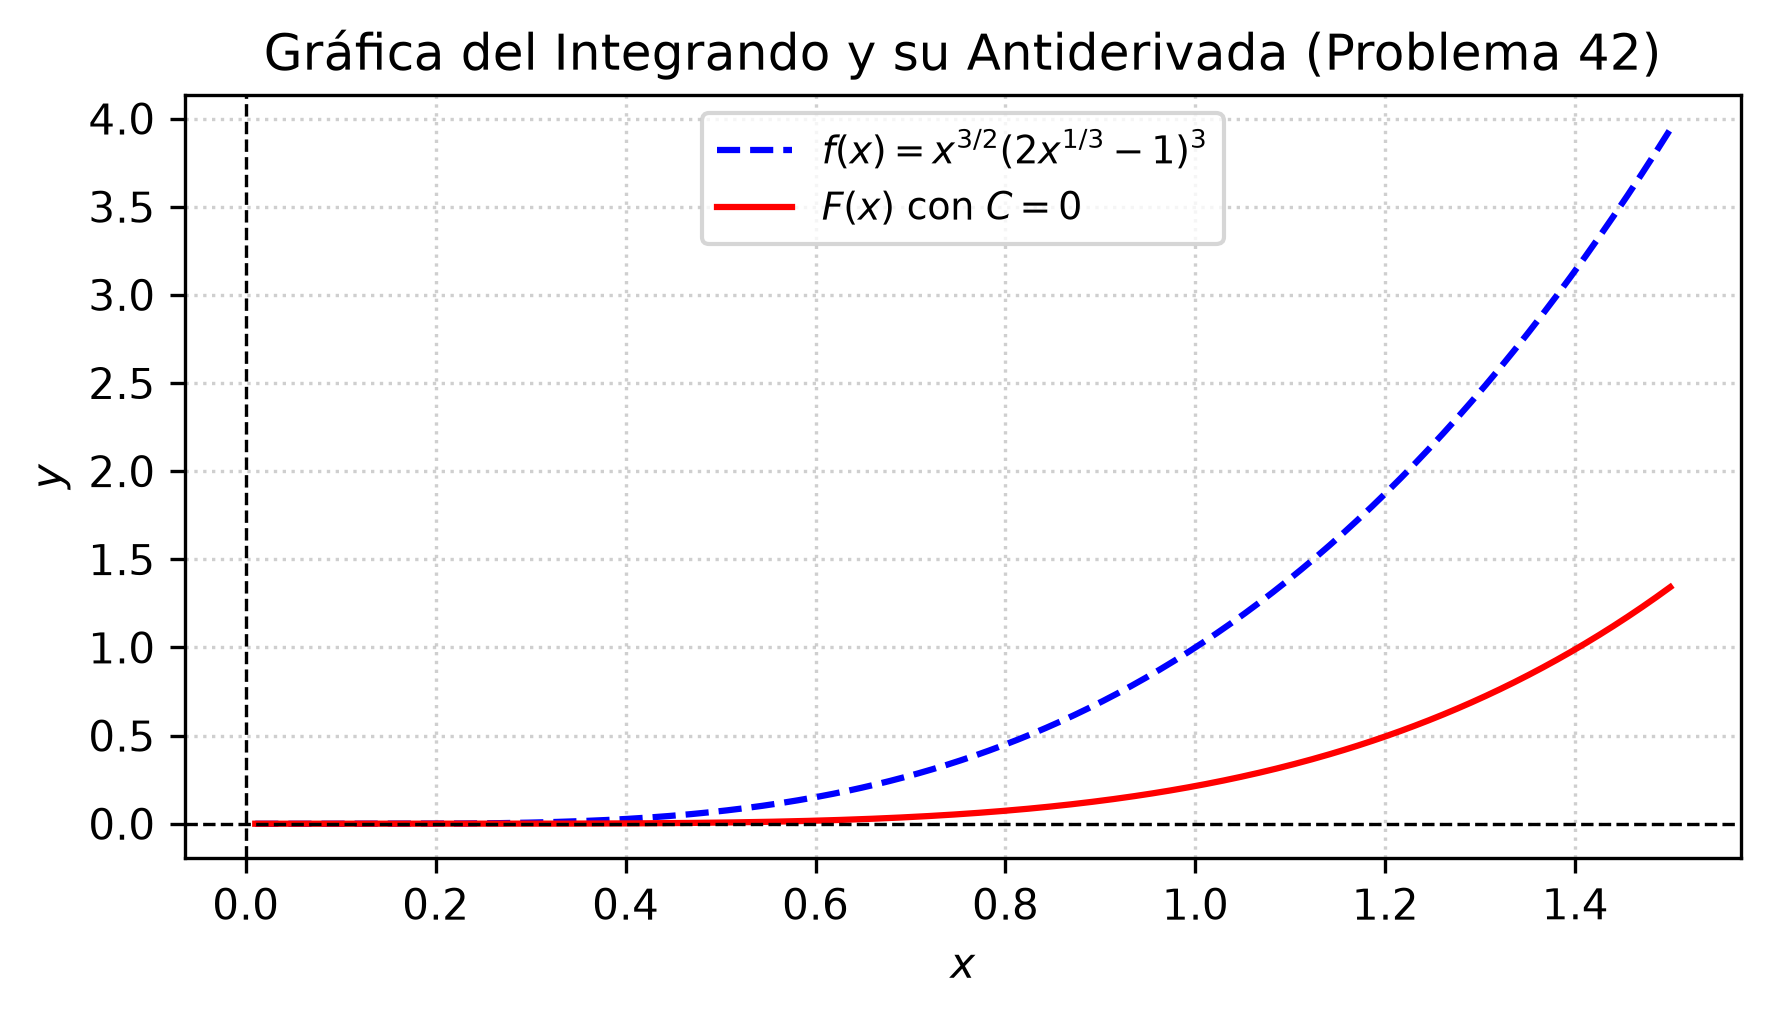
\includegraphics[width=\columnwidth]{semana_05/graficas/SEM05_P42_grafica.png}
	\caption{Representación gráfica de $f(x)$ y su antiderivada $F(x)$ evaluada para la constante de integración $C = 0$ (Problema 42).}
	\label{fig:problema42}
\end{figure}

	\subsection*{Problema 43}

\textbf{Enunciado:} \\
Calcular la integral indefinida:
\begin{align*}
\int x^3 (1 - x^2)^{-3/2} \, dx
\end{align*}

\textbf{Solución:} \\
Para resolver esta integral, utilizaremos el método de sustitución algebraica. 
Definimos la nueva variable $u$ y su respectiva derivada de la siguiente manera:
\begin{align*}
u &= 1 - x^2 \\
du &= -2x \, dx \implies x \, dx = -\dfrac{1}{2} \, du
\end{align*}

De la definición de $u$, podemos expresar $x^2$ en términos de $u$:
\begin{align*}
x^2 = 1 - u
\end{align*}

Reescribimos la integral original separando un término $x$ para construir la expresión $x \, dx$:
\begin{align*}
\int x^2 \cdot (1 - x^2)^{-3/2} \cdot (x \, dx)
\end{align*}

Sustituimos $x^2$, $1 - x^2$ y $x \, dx$ en la integral:
\begin{align*}
\int (1 - u) \cdot (u)^{-3/2} \cdot \left(-\dfrac{1}{2} \, du\right)
\end{align*}

Sacamos la constante fuera de la integral y distribuimos el término $u^{-3/2}$:
\begin{align*}
-\dfrac{1}{2} \int (u^{-3/2} - u^{-1/2}) \, du
\end{align*}

Integramos término a término usando la regla de la potencia:
\begin{align*}
&= -\dfrac{1}{2} \left[ \dfrac{u^{-1/2}}{-1/2} - \dfrac{u^{1/2}}{1/2} \right] \\
&= -\dfrac{1}{2} \left[ -2u^{-1/2} - 2u^{1/2} \right]
\end{align*}

Simplificamos el factor escalar $-\dfrac{1}{2}$ con el paréntesis:
\begin{align*}
&= u^{-1/2} + u^{1/2} + C \\
&= \dfrac{1}{\sqrt{u}} + \sqrt{u} + C
\end{align*}

Finalmente, regresamos a la variable original $x$ sustituyendo $u = 1 - x^2$:
\begin{align*}
&= \dfrac{1}{\sqrt{1 - x^2}} + \sqrt{1 - x^2} + C
\end{align*}

Podemos expresar el resultado bajo un mismo denominador común:
\begin{align*}
&= \dfrac{1 + (1 - x^2)}{\sqrt{1 - x^2}} + C \\
&= \dfrac{2 - x^2}{\sqrt{1 - x^2}} + C
\end{align*}

\begin{figure}[H]
	\centering
	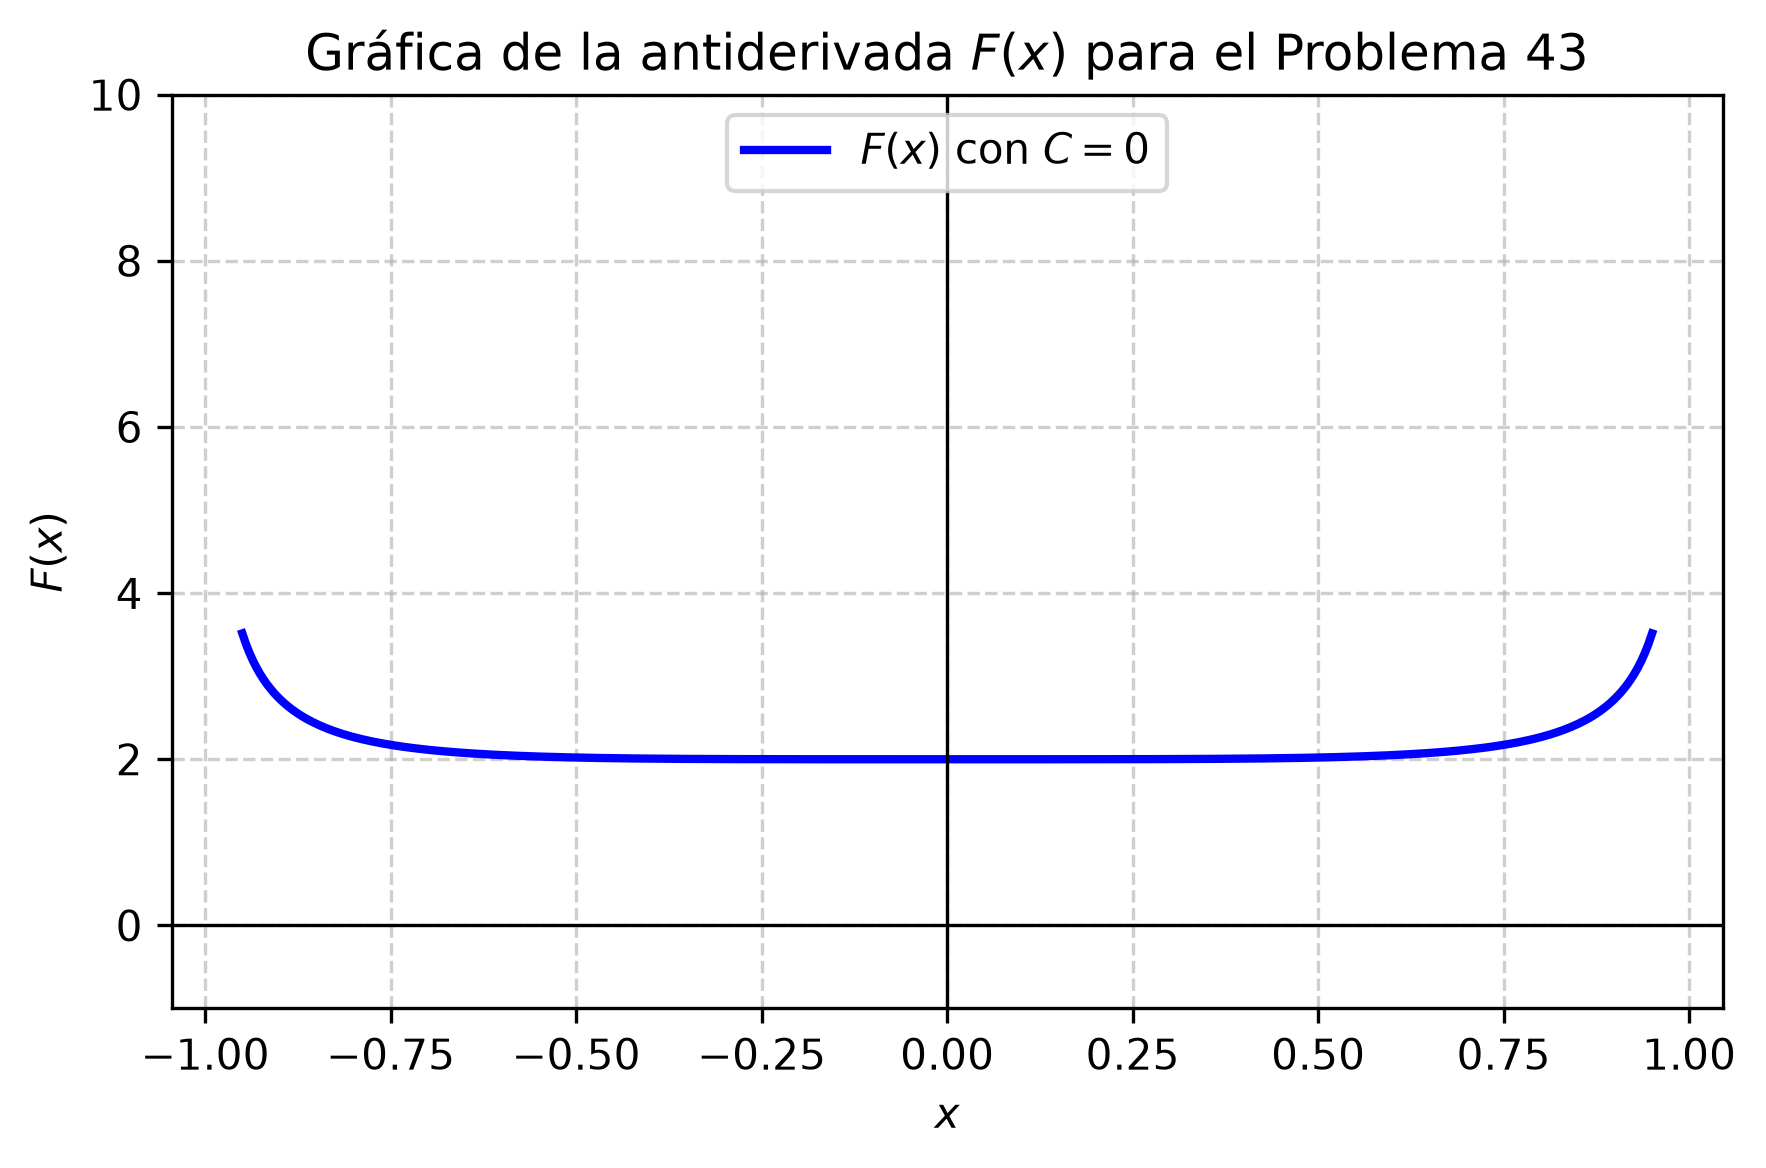
\includegraphics[width=\columnwidth]{semana_05/graficas/SEM05_P43_grafica.png}
	\caption{Representación gráfica de $f(x)$ y su antiderivada $F(x)$ evaluada para la constante de integración $C = 0$ (Problema 43).}
	\label{fig:problema43}
\end{figure}

	\subsection*{Problema 44}

\textbf{Enunciado:} Calcular la integral indefinida
\begin{align*}
I = \int x^3 (1 + x^2)^{-1/2} \, dx
\end{align*}

\textbf{Solución:} 
Siguiendo las indicaciones, aplicamos la sustitución $u = 1 + x^2$. 
Derivando ambos lados, obtenemos $du = 2x \, dx$, lo que implica que:
\begin{align*}
x \, dx = \dfrac{1}{2} \, du
\end{align*}

Además, de la definición de $u$, despejamos $x^2$:
\begin{align*}
x^2 = u - 1
\end{align*}

Reescribimos el integrando original separando un factor $x$ para aplicar la sustitución:
\begin{align*}
I &= \int x^2 (1 + x^2)^{-1/2} (x \, dx) \\
I &= \int (u - 1) u^{-1/2} \left(\dfrac{1}{2} \, du\right) \\
I &= \dfrac{1}{2} \int (u - 1) u^{-1/2} \, du
\end{align*}

Multiplicando el término $u^{-1/2}$ por cada componente del binomio, descomponemos la integral en dos potencias simples:
\begin{align*}
I &= \dfrac{1}{2} \int \left( u^{1/2} - u^{-1/2} \right) du
\end{align*}

Integramos cada término utilizando la regla de la potencia:
\begin{align*}
I &= \dfrac{1}{2} \left[ \dfrac{u^{3/2}}{3/2} - \dfrac{u^{1/2}}{1/2} \right] + C \\
I &= \dfrac{1}{2} \left[ \dfrac{2}{3} u^{3/2} - 2 u^{1/2} \right] + C \\
I &= \dfrac{1}{3} u^{3/2} - u^{1/2} + C
\end{align*}

Factorizando $u^{1/2}$ y devolviendo la variable original $u = 1 + x^2$:
\begin{align*}
I &= u^{1/2} \left( \dfrac{1}{3}u - 1 \right) + C \\
I &= (1 + x^2)^{1/2} \left[ \dfrac{1}{3}(1 + x^2) - 1 \right] + C \\
I &= (1 + x^2)^{1/2} \left( \dfrac{x^2 - 2}{3} \right) + C
\end{align*}

Por lo tanto, el resultado de la integral es:
\begin{align*}
I = \dfrac{(x^2 - 2)\sqrt{1 + x^2}}{3} + C
\end{align*}

\begin{figure}[H]
	\centering
	
\includegraphics[width=\columnwidth]{semana_05/graficas/SEM05_P44_grafica.png}
	\caption{Representación gráfica de $f(x)$ y su antiderivada $F(x)$ evaluada para la constante de integración $C = 0$ (Problema 44).}
	\label{fig:problema44}
\end{figure}

	\subsection*{Problema 45}

\textbf{Enunciado:}
Calcular la integral indefinida:
\begin{align*}
\int \dfrac{x}{\sqrt{x - 1}} \, dx
\end{align*}

\textbf{Solución:}
Para resolver la integral, aplicamos el método de sustitución recomendado. Definimos la nueva variable $u$:
\begin{align*}
u &= \sqrt{x - 1}
\end{align*}

Elevamos al cuadrado ambos lados para despejar la variable $x$:
\begin{align*}
u^2 &= x - 1 \\
x &= u^2 + 1
\end{align*}

Ahora, encontramos el diferencial $dx$ derivando la expresión de $x$ con respecto a $u$:
\begin{align*}
dx &= 2u \, du
\end{align*}

Sustituimos $x$, $\sqrt{x-1}$ y $dx$ en la integral original:
\begin{align*}
\int \dfrac{u^2 + 1}{u} (2u \, du)
\end{align*}

Simplificamos la expresión algebraica cancelando $u$ y extrayendo las constantes:
\begin{align*}
&= \int (u^2 + 1)(2) \, du \\
&= 2 \int (u^2 + 1) \, du
\end{align*}

integramos término a término usando la regla de la potencia:
\begin{align*}
&= 2 \left( \dfrac{u^3}{3} + u \right) + C
\end{align*}

Distribuimos el factor 2:
\begin{align*}
&= \dfrac{2}{3}u^3 + 2u + C
\end{align*}

Finalmente, regresamos a la variable original $x$ sustituyendo $u = \sqrt{x - 1}$:
\begin{align*}
&= \dfrac{2}{3}(\sqrt{x - 1})^3 \\
&\quad + 2\sqrt{x - 1} + C
\end{align*}

Agrupando el resultado, la solución general es:
\begin{align*}
\int \dfrac{x}{\sqrt{x - 1}} \, dx = \dfrac{2}{3}(x - 1)^{\frac{3}{2}} \\
+ 2(x - 1)^{\frac{1}{2}} + C
\end{align*}

\begin{figure}[H]
	\centering
	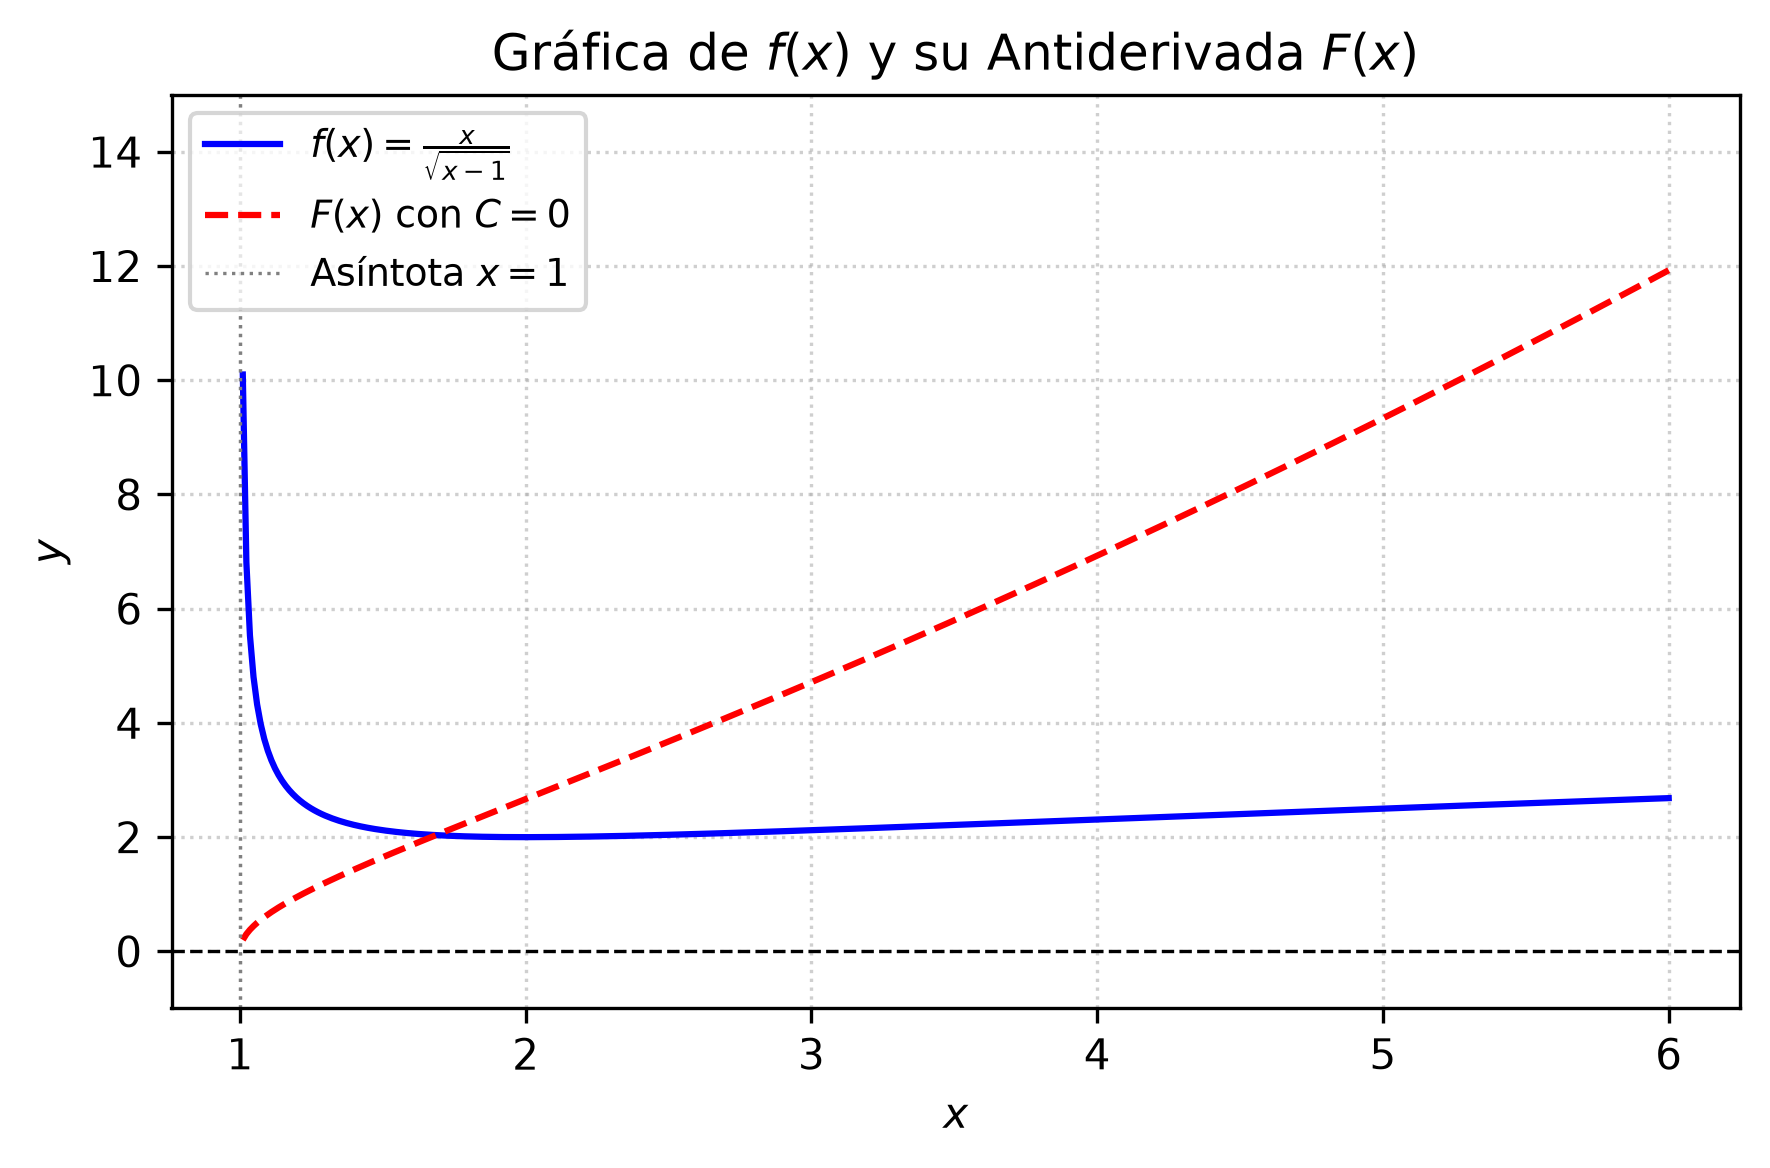
\includegraphics[width=\columnwidth]{semana_05/graficas/SEM05_P45_grafica.png}
	\caption{Representación gráfica de $f(x)$ y su antiderivada $F(x)$ evaluada para la constante de integración $C = 0$ (Problema 45).}
	\label{fig:problema45}
\end{figure}

	\subsection*{Problema 46}
\textbf{Enunciado:} Calcular la integral:
\begin{align*}
\int (4x^2 + 4x - 3)^{-1/2} \, dx
\end{align*}

\textbf{Solución:}
Primero, expresamos la integral con el radical en el denominador:
\begin{align*}
\int \dfrac{1}{\sqrt{4x^2 + 4x - 3}} \, dx
\end{align*}

Completamos el cuadrado en el trinomio dentro de la raíz. Factorizamos el coeficiente principal del término cuadrático:
\begin{align*}
4x^2 + 4x - 3 &= 4\left(x^2 + x - \dfrac{3}{4}\right)
\end{align*}

Completamos el trinomio cuadrado perfecto sumando y restando $(1/2)^2 = 1/4$:
\begin{align*}
4\left[\left(x^2 + x + \dfrac{1}{4}\right) - \dfrac{1}{4} - \dfrac{3}{4}\right] &= 4\left[\left(x + \dfrac{1}{2}\right)^2 - 1\right]
\end{align*}

Distribuimos el factor $4$:
\begin{align*}
4\left(x + \dfrac{1}{2}\right)^2 - 4 &= (2x + 1)^2 - 4
\end{align*}

Sustituimos la expresión completada en la integral original:
\begin{align*}
\int \dfrac{1}{\sqrt{(2x + 1)^2 - 4}} \, dx
\end{align*}

Realizamos la sustitución: sea $u = 2x + 1$, de donde $du = 2 \, dx$, lo que implica que $dx = \frac{1}{2} \, du$. La integral se transforma en:
\begin{align*}
\dfrac{1}{2} \int \dfrac{1}{\sqrt{u^2 - 4}} \, du
\end{align*}

Utilizamos la fórmula estándar de integración para funciones con radicales de la forma $\sqrt{u^2 - a^2}$:
\begin{align*}
\int \dfrac{1}{\sqrt{u^2 - a^2}} \, du = \ln\left|u + \sqrt{u^2 - a^2}\right| + C
\end{align*}

Aplicando la fórmula con $a = 2$:
\begin{align*}
\dfrac{1}{2} \ln\left|u + \sqrt{u^2 - 4}\right| + C_1
\end{align*}

Regresamos a la variable original $x$ sustituyendo $u = 2x + 1$:
\begin{align*}
\dfrac{1}{2} \ln\Big|2x + 1 &+ \sqrt{(2x + 1)^2 - 4}\Big| + C_1
\end{align*}

Simplificamos el argumento dentro del radical para obtener la forma final:
\begin{align*}
\dfrac{1}{2} \ln\Big|2x + 1 &+ \sqrt{4x^2 + 4x - 3}\Big| + C
\end{align*}

\begin{figure}[H]
	\centering
	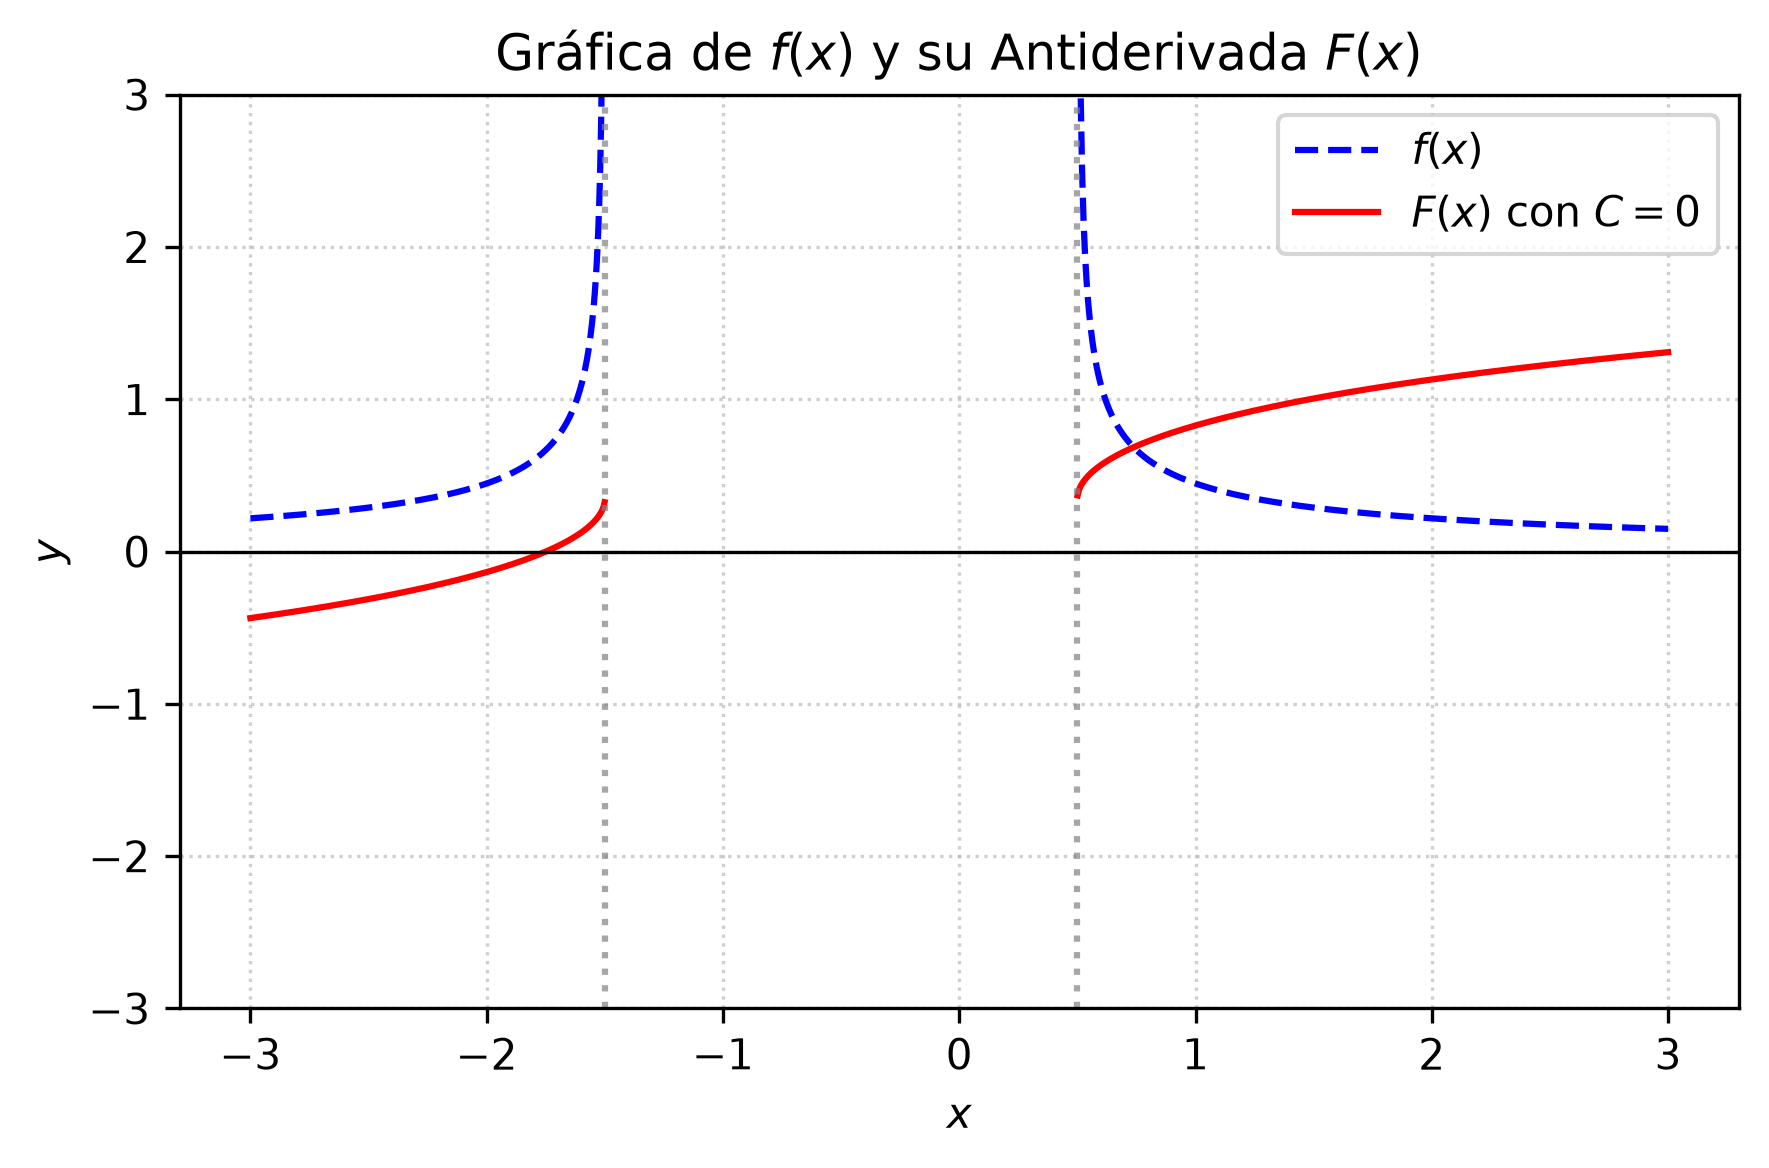
\includegraphics[width=\columnwidth]{semana_05/graficas/SEM05_P46_grafica.png}
	\caption{Representación gráfica de $f(x)$ y su antiderivada $F(x)$ evaluada para la constante de integración $C = 0$ (Problema 46).}
	\label{fig:problema46}
\end{figure}

	\subsection*{Problema 47}
\textbf{Enunciado:} Calcular la integral:
\begin{equation*}
\int \sqrt{4x^2 + 4x - 3} \, dx
\end{equation*}

\textbf{Solución:}
Primero, completamos el cuadrado dentro de la raíz para la expresión cuadrática.
Agrupamos los términos en $x$:
\begin{align*}
4x^2 + 4x - 3 &= 4(x^2 + x) - 3 \\
&= 4\left(x^2 + x + \dfrac{1}{4} - \dfrac{1}{4}\right) - 3 \\
&= 4\left(x + \dfrac{1}{2}\right)^2 - 1 - 3 \\
&= 4\left(x + \dfrac{1}{2}\right)^2 - 4
\end{align*}

Sustituimos esta forma en la integral original:
\begin{align*}
\int &\sqrt{4x^2 + 4x - 3} \, dx \\
&= \int \sqrt{4\left(x + \dfrac{1}{2}\right)^2 - 4} \, dx \\
&= \int 2\sqrt{\left(x + \dfrac{1}{2}\right)^2 - 1} \, dx
\end{align*}

Utilizamos la sustitución trigonométrica. 
Sea $x + \dfrac{1}{2} = \sec\theta$, de modo que 
$dx = \sec\theta \tan\theta \, d\theta$.
Además, la raíz se simplifica como:
\begin{align*}
\sqrt{\left(x + \dfrac{1}{2}\right)^2 - 1} &= \sqrt{\sec^2\theta - 1} \\
&= \tan\theta
\end{align*}

Sustituyendo en la integral:
\begin{align*}
\int &2(\tan\theta)(\sec\theta \tan\theta) \, d\theta \\
&= 2 \int \sec\theta \tan^2\theta \, d\theta \\
&= 2 \int \sec\theta (\sec^2\theta - 1) \, d\theta \\
&= 2 \int (\sec^3\theta - \sec\theta) \, d\theta
\end{align*}

Empleamos la fórmula de reducción para $\sec^3\theta$:
\begin{align*}
2 \left[ \dfrac{1}{2}\sec\theta\tan\theta + \dfrac{1}{2}\ln|\sec\theta + \tan\theta| \right. \\
\left. - \ln|\sec\theta + \tan\theta| \right] + C
\end{align*}

Simplificando los términos obtenemos:
\begin{align*}
= \sec\theta\tan\theta - \ln|\sec\theta + \tan\theta| + C
\end{align*}

Regresamos a la variable original $x$ usando $\sec\theta = x + \dfrac{1}{2}$ y $\tan\theta = \sqrt{4x^2 + 4x - 3}/2$:
\begin{align*}
&= \left(x + \dfrac{1}{2}\right)\dfrac{\sqrt{4x^2 + 4x - 3}}{2} \\
&\quad - \ln\left|x + \dfrac{1}{2} + \dfrac{\sqrt{4x^2 + 4x - 3}}{2}\right| + C
\end{align*}

\begin{figure}[H]
	\centering
	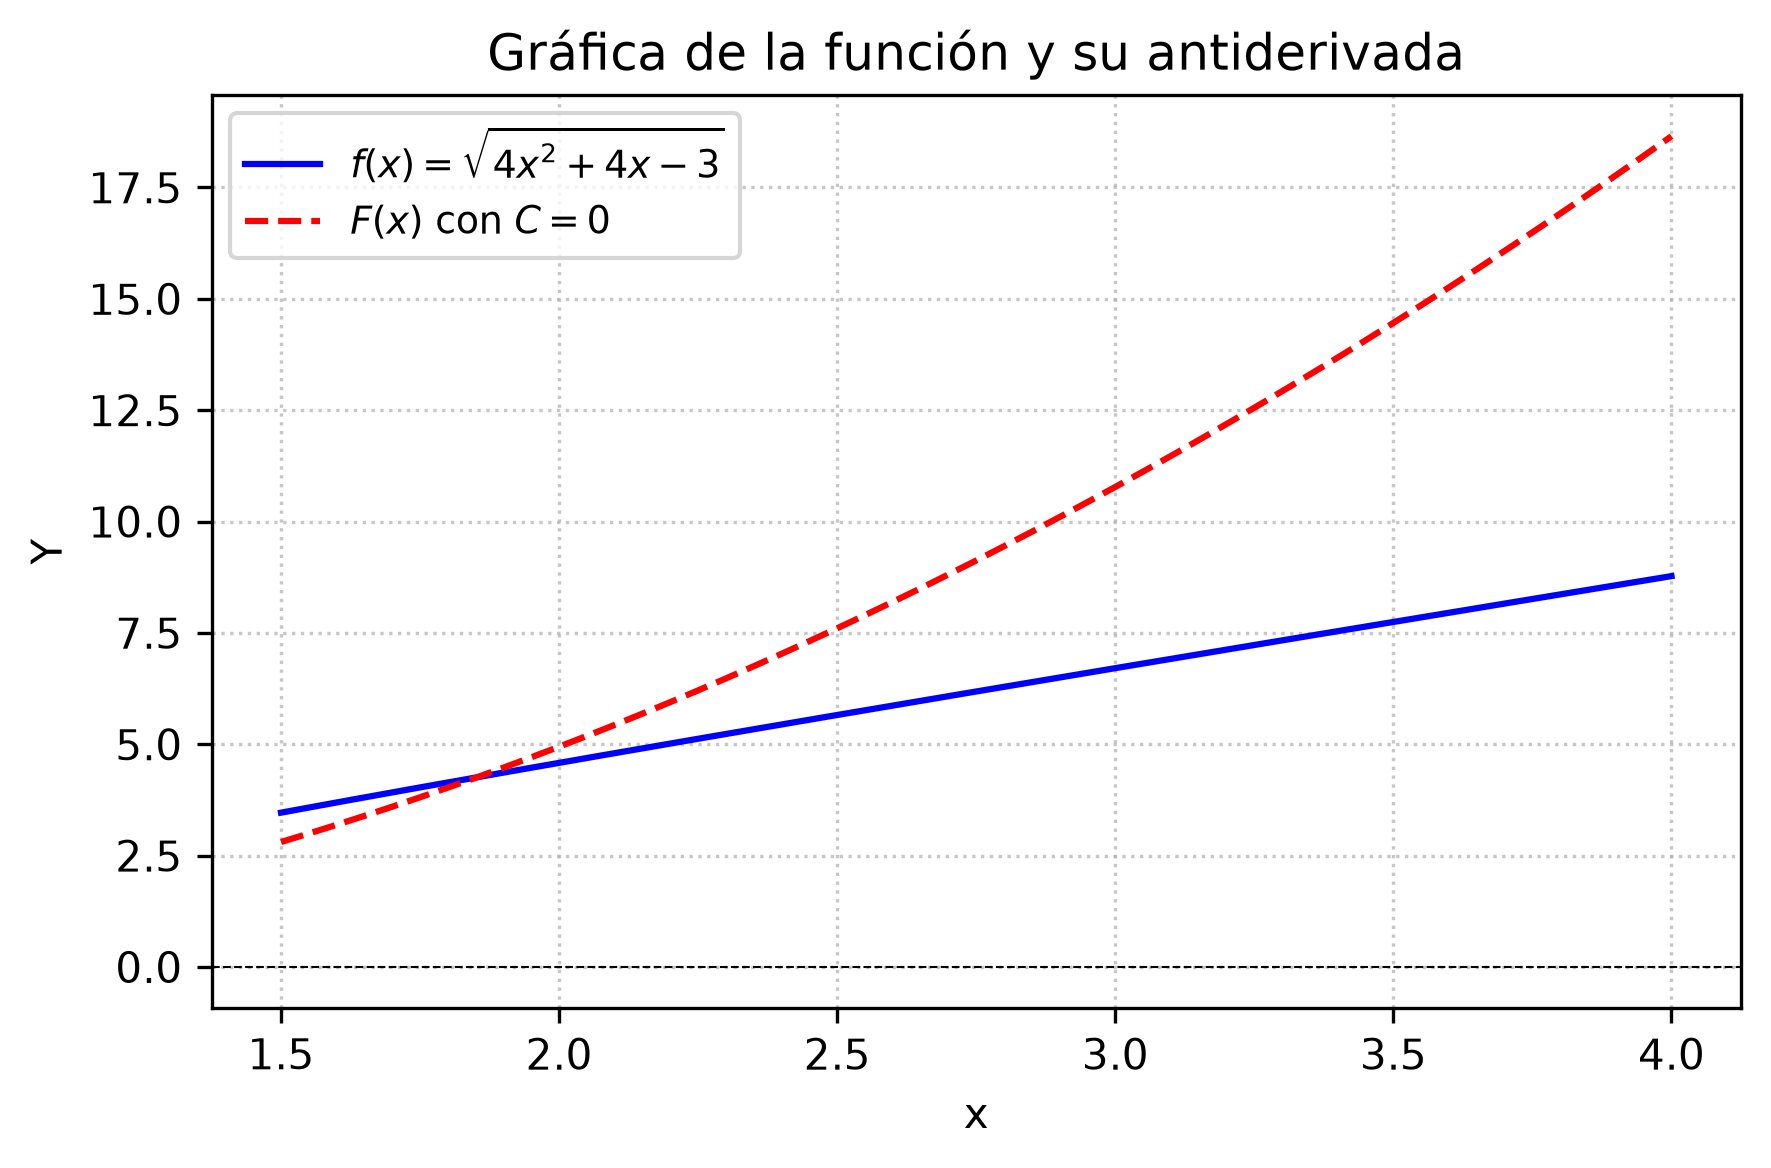
\includegraphics[width=\columnwidth]{semana_05/graficas/SEM05_P47_grafica.png}
	\caption{Representación gráfica de $f(x)$ y su antiderivada $F(x)$ evaluada para la constante de integración $C = 0$ (Problema 47).}
	\label{fig:problema47}
\end{figure}

	\subsection*{Problema 48}

\textbf{Enunciado:}
Calcular la siguiente integral indefinida:
\begin{align*}
\int \frac{x}{\sqrt{x^2 + 2x + 2}} \, dx
\end{align*}

\textbf{Solución:}

Siguiendo la indicación, el objetivo es expresar el numerador en función de la derivada de la cantidad subradical. Sea $u = x^2 + 2x + 2$, su derivada es $du = (2x + 2) \, dx$. 

Manipulamos algebraicamente el numerador de la integral para que aparezca dicha derivada:
\begin{align*}
x &= \dfrac{1}{2}(2x) \\
&= \dfrac{1}{2}(2x + 2 - 2) \\
&= \dfrac{1}{2}(2x + 2) - 1
\end{align*}

Sustituimos esta expresión en el numerador de la integral original:
\begin{align*}
\int &\dfrac{x}{\sqrt{x^2 + 2x + 2}} \, dx = \\
&\int \dfrac{\frac{1}{2}(2x + 2) - 1}{\sqrt{x^2 + 2x + 2}} \, dx
\end{align*}

Separamos la integral en dos partes distintas:
\begin{align*}
&= \dfrac{1}{2} \int \dfrac{2x + 2}{\sqrt{x^2 + 2x + 2}} \, dx \\
&\quad - \int \dfrac{1}{\sqrt{x^2 + 2x + 2}} \, dx
\end{align*}

Para la primera integral, usamos sustitución directa con $u = x^2 + 2x + 2$ y $du = (2x + 2) \, dx$:
\begin{align*}
I_1 &= \dfrac{1}{2} \int u^{-1/2} \, du \\
&= \dfrac{1}{2} \left( 2u^{1/2} \right) = \sqrt{u} \\
&= \sqrt{x^2 + 2x + 2}
\end{align*}

Para la segunda integral, completamos el trinomio cuadrado perfecto en el denominador:
\begin{align*}
x^2 + 2x + 2 &= (x^2 + 2x + 1) + 1 \\
&= (x + 1)^2 + 1
\end{align*}

Sustituimos esto en la segunda integral $I_2$:
\begin{align*}
I_2 &= \int \dfrac{1}{\sqrt{(x + 1)^2 + 1}} \, dx
\end{align*}

Esta integral se resuelve mediante la fórmula estándar de sustitución trigonométrica o integración directa con funciones hiperbólicas/logarítmicas:
\begin{align*}
I_2 &= \ln\left| (x + 1) + \sqrt{(x + 1)^2 + 1} \right| \\
&= \ln\left| x + 1 + \sqrt{x^2 + 2x + 2} \right|
\end{align*}

Finalmente, combinamos ambos resultados y añadimos la constante de integración $C$:
\begin{align*}
\int &\dfrac{x}{\sqrt{x^2 + 2x + 2}} \, dx = \sqrt{x^2 + 2x + 2} \\
&\quad - \ln\left| x + 1 + \sqrt{x^2 + 2x + 2} \right| + C
\end{align*}

\begin{figure}[H]
	\centering
	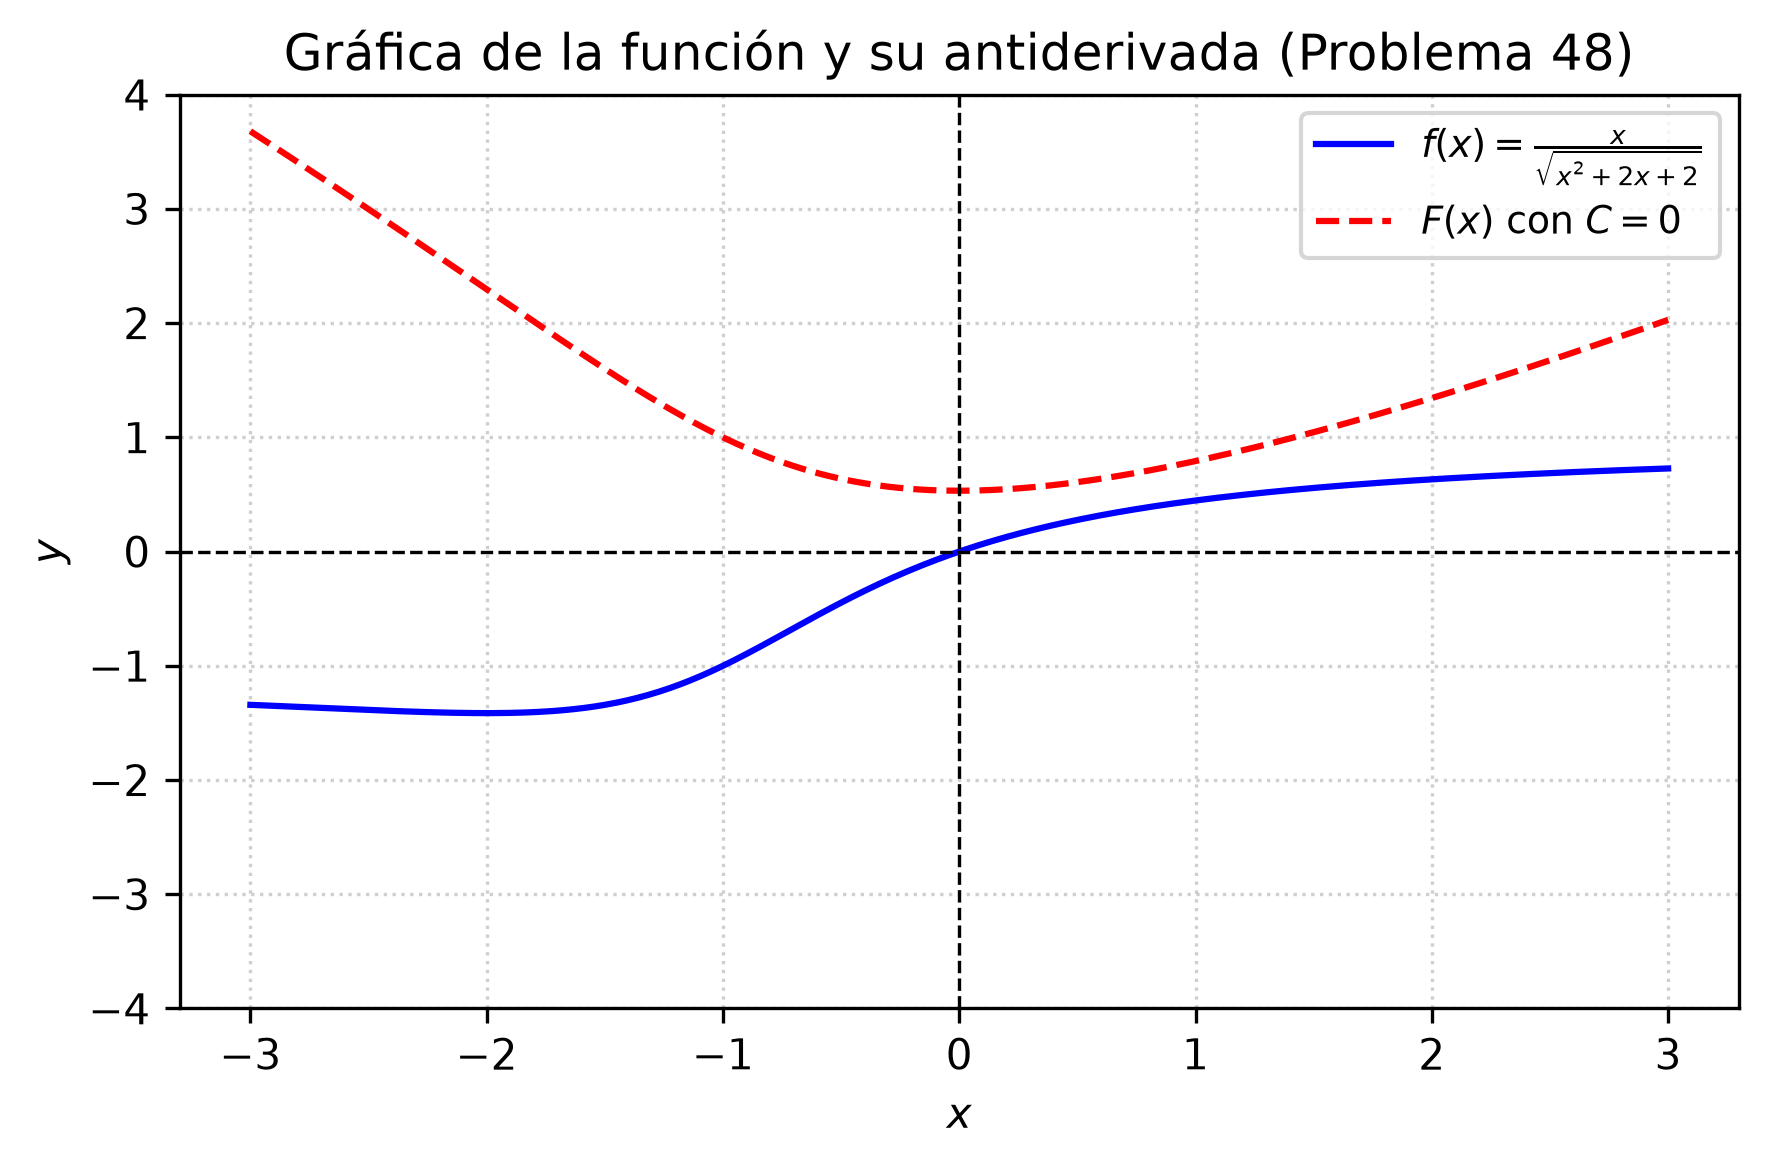
\includegraphics[width=\columnwidth]{semana_05/graficas/SEM05_P48_grafica.png}
	\caption{Representación gráfica de $f(x)$ y su antiderivada $F(x)$ evaluada para la constante de integración $C = 0$ (Problema 48).}
	\label{fig:problema48}
\end{figure}

	\subsection*{Problema 49}
\textbf{Enunciado:} Calcular la integral:
\begin{align*}
\int \dfrac{1}{x \sqrt{1 + x - x^2}} \, dx
\end{align*}

\textbf{Solución:} Para resolver la integral dada, utilizamos la sustitución recíproca sugerida. Sea:
\begin{align*}
u = \dfrac{1}{x} \implies x = \dfrac{1}{u}
\end{align*}

Calculamos el diferencial $dx$:
\begin{align*}
dx = -\dfrac{1}{u^2} \, du
\end{align*}

Sustituimos $x$ y $dx$ en la integral original:
\begin{align*}
\int \dfrac{1}{\left(\dfrac{1}{u}\right) \sqrt{1 + \dfrac{1}{u} - \left(\dfrac{1}{u}\right)^2}} \left(-\dfrac{1}{u^2} \, du\right)
\end{align*}

Simplificamos la expresión algebraica dentro del integrando:
\begin{align*}
= -\int \dfrac{\dfrac{1}{u^2}}{\left(\dfrac{1}{u}\right) \sqrt{1 + \dfrac{1}{u} - \dfrac{1}{u^2}}} \, du
\end{align*}

\begin{align*}
= -\int \dfrac{1}{u \sqrt{\dfrac{u^2 + u - 1}{u^2}}} \, du
\end{align*}

Como $u > 0$ en el dominio de interés, extraemos la raíz del denominador:
\begin{align*}
= -\int \dfrac{1}{u \left(\dfrac{\sqrt{u^2 + u - 1}}{u}\right)} \, du
\end{align*}

\begin{align*}
= -\int \dfrac{1}{\sqrt{u^2 + u - 1}} \, du
\end{align*}

Completamos el trinomio cuadrado perfecto bajo el radical:
\begin{align*}
u^2 + u - 1 &= \left(u^2 + u + \dfrac{1}{4}\right) - \dfrac{1}{4} - 1 \\
&= \left(u + \dfrac{1}{2}\right)^2 - \dfrac{5}{4}
\end{align*}

Sustituimos esto en la integral:
\begin{align*}
= -\int \dfrac{1}{\sqrt{\left(u + \dfrac{1}{2}\right)^2 - \left(\dfrac{\sqrt{5}}{2}\right)^2}} \, du
\end{align*}

Utilizamos la fórmula estándar de integración:
\begin{align*}
\int \dfrac{1}{\sqrt{z^2 - a^2}} \, dz = \ln\left|z + \sqrt{z^2 - a^2}\right| + C
\end{align*}

Aplicando la fórmula con $z = u + \dfrac{1}{2}$ y $a = \dfrac{\sqrt{5}}{2}$:
\begin{align*}
= -\ln\left|u + \dfrac{1}{2} + \sqrt{u^2 + u - 1}\right| + C
\end{align*}

Finalmente, regresamos a la variable original $x$ sustituyendo $u = \dfrac{1}{x}$:
\begin{align*}
= -\ln\left|\dfrac{1}{x} + \dfrac{1}{2} + \sqrt{\dfrac{1}{x^2} + \dfrac{1}{x} - 1}\right| + C
\end{align*}

\begin{figure}[H]
	\centering
	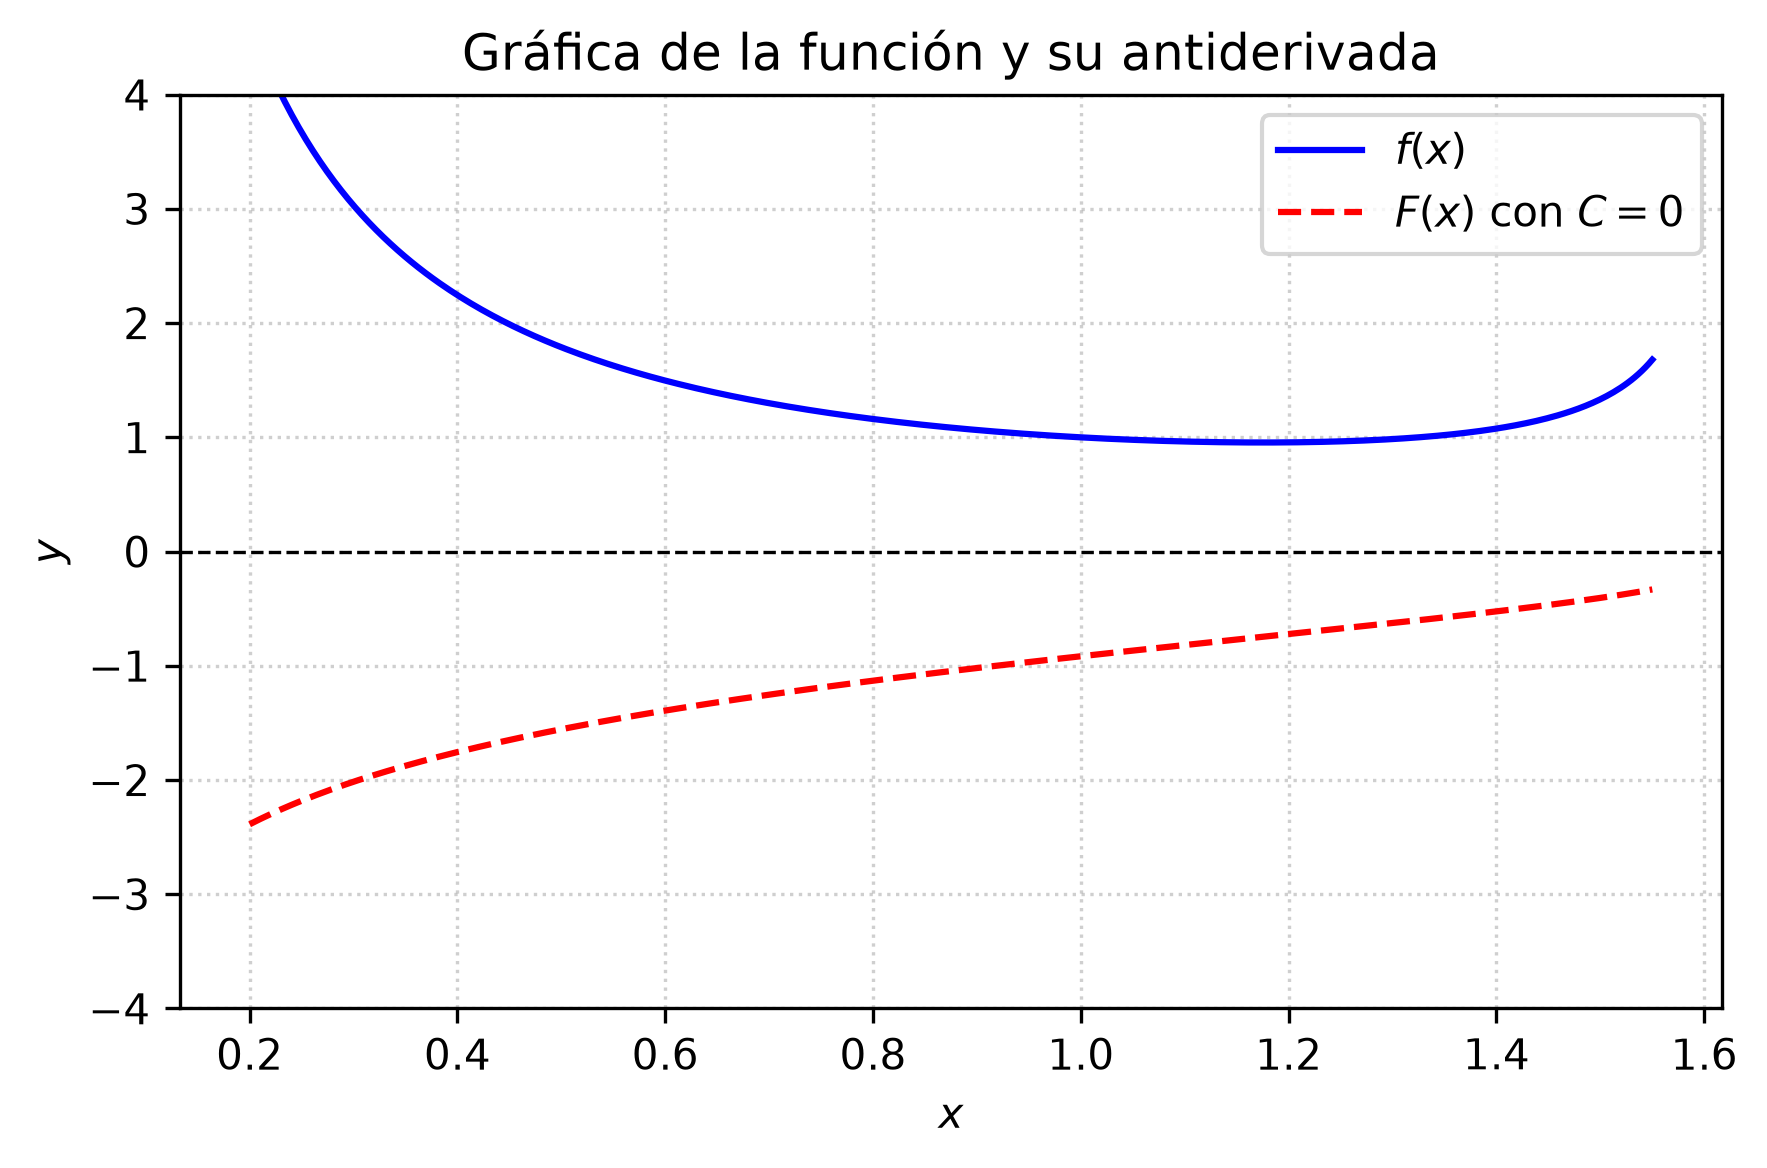
\includegraphics[width=\columnwidth]{semana_05/graficas/SEM05_P49_grafica.png}
	\caption{Representación gráfica de $f(x)$ y su antiderivada $F(x)$ evaluada para la constante de integración $C = 0$ (Problema 49).}
	\label{fig:problema49}
\end{figure}

	%\input{semana_05/tex_soluciones/SEM05_P50_solucion.tex}
	%\input{semana_03/tex_soluciones/SEM03_P51_solucion.tex}
	%\input{semana_03/tex_soluciones/SEM03_P52_solucion.tex}
	%\input{semana_03/tex_soluciones/SEM03_P53_solucion.tex}
	%\input{semana_03/tex_soluciones/SEM03_P54_solucion.tex}
	%\input{semana_03/tex_soluciones/SEM03_P55_solucion.tex}
	%\input{semana_03/tex_soluciones/SEM03_P56_solucion.tex}
	%\input{semana_03/tex_soluciones/SEM03_P57_solucion.tex}
	%\input{semana_03/tex_soluciones/SEM03_P58_solucion.tex}
	%\input{semana_03/tex_soluciones/SEM03_P59_solucion.tex}
	%\input{semana_03/tex_soluciones/SEM03_P60_solucion.tex}
	%\input{semana_03/tex_soluciones/SEM03_P61_solucion.tex}
	%\input{semana_03/tex_soluciones/SEM03_P62_solucion.tex}
	%\input{semana_03/tex_soluciones/SEM03_P63_solucion.tex}
	%\input{semana_03/tex_soluciones/SEM03_P64_solucion.tex}
	%\input{semana_03/tex_soluciones/SEM03_P65_solucion.tex}
	%\input{semana_03/tex_soluciones/SEM03_P66_solucion.tex}
	%\input{semana_03/tex_soluciones/SEM03_P67_solucion.tex}
	%\input{semana_03/tex_soluciones/SEM03_P68_solucion.tex}
	%\input{semana_03/tex_soluciones/SEM03_P69_solucion.tex}
	%\input{semana_03/tex_soluciones/SEM03_P70_solucion.tex}
	%\input{semana_03/tex_soluciones/SEM03_P71_solucion.tex}
	%\input{semana_03/tex_soluciones/SEM03_P72_solucion.tex}
	%\input{semana_03/tex_soluciones/SEM03_P73_solucion.tex}
	%\input{semana_03/tex_soluciones/SEM03_P74_solucion.tex}
	%\input{semana_03/tex_soluciones/SEM03_P75_solucion.tex}
	%\input{semana_03/tex_soluciones/SEM03_P76_solucion.tex}
	%\input{semana_03/tex_soluciones/SEM03_P77_solucion.tex}
	%\input{semana_03/tex_soluciones/SEM03_P78_solucion.tex}
	%\input{semana_03/tex_soluciones/SEM03_P79_solucion.tex}
	%\input{semana_03/tex_soluciones/SEM03_P80_solucion.tex}
	
\end{document}